\documentclass[11pt,a4paper]{report}
\usepackage[T1]{fontenc}
\usepackage{lmodern}
\usepackage[margin=2.3cm]{geometry}
\usepackage{amsmath,amssymb}
\usepackage{booktabs,longtable,array}
\usepackage{listings}
\usepackage{xcolor}
\usepackage{graphicx}
\usepackage{tikz}
\usetikzlibrary{positioning,arrows.meta,shapes.geometric}
\PassOptionsToPackage{obeyspaces}{url}
\usepackage[colorlinks=true,linkcolor=blue!50!black,urlcolor=blue!50!black]{hyperref}
\setlength{\parskip}{0.55em}
\setlength{\parindent}{0pt}
\makeatletter
\g@addto@macro\UrlBreaks{\do\_\do\-\do\,\do\=\do\<\do\>\do\ }
\makeatother
\urlstyle{tt}
\newcommand{\code}[1]{\path{#1}}
\sloppy
\emergencystretch=3em
\lstset{basicstyle=\ttfamily\footnotesize,breaklines=true,columns=fullflexible,
  frame=single,framerule=0.3pt,rulecolor=\color[gray]{0.6},xleftmargin=2pt,xrightmargin=2pt,
  aboveskip=0.8em,belowskip=0.6em,showstringspaces=false}
\newenvironment{tip}{\begin{center}\begin{tabular}{|p{0.92\textwidth}|}\hline\small\textbf{Tip.}~}{\\\hline\end{tabular}\end{center}}
\setcounter{secnumdepth}{2}
\setcounter{tocdepth}{1}

\title{\textbf{Statistical validation of TESS and Kepler candidates}\\[0.4em]
\Large TRICERATOPS validation pipeline --- Observer's Guide\\[0.3em]
\large with the graphical user interface}
\date{Pipeline \texttt{triceratops\_validation.py} v4.3 \quad GUI \texttt{triceratops\_gui.py} v1.2 \quad Audit \texttt{triceratops\_audit.py} v0.1\\[0.3em] November 2026}
\author{}

\input{glyphtounicode}
\pdfgentounicode=1
\begin{document}
\maketitle

\begin{abstract}
This guide is written for observers and collaborators who want to use the
validation pipeline without reading its 170-page technical manual. Part~I
explains what TRICERATOPS computes, which false-positive scenarios it
considers, what the pipeline adds around it, how ground-based photometry
enters the analysis, and how the audit turns the result into a recommendation
for the next observations. Part~II explains the graphical user interface (GUI)
with a worked example, the AAVSO campaign 942 on TIC~65344135, gives the
TESS-only result for that star and its recommended follow-up, tests the
pipeline on the known hot Jupiter WASP-18~b, unmasks the two candidates of
TIC~229701403 as one eccentric eclipsing binary, discusses the M-dwarf
candidate L~279-94 and its habitable-zone question, and shows how Kepler
targets are analysed. It ends with a complete reference of all
options, the output files and common problems. The technical manual
(\code{TRICERATOPS_Validation_Pipeline_Documentation_v4.3.pdf}) remains the
reference for the methods and their tests.

\textbf{New in v4.3:} Kepler targets (v4.2); fixes from the independent test
runs of Steve Price (KESTREL); a verdict that also listens to the pipeline's
own eclipsing-binary tests; the audit with its page \emph{Next observations}
(Chapter~\ref{ch:followup}); the control target WASP-18~b with its
secondary eclipse (Chapter~\ref{ch:wasp18}); the false positive
TIC~229701403 (Chapter~\ref{ch:tic2297}); the M-dwarf candidate L~279-94
(Chapter~\ref{ch:l27994}); multi-band light curves with
TRICERATOPS+ and the audit's colour test (Section~\ref{sec:multiband}).
\end{abstract}

\tableofcontents

%% ======================================================================
\part{Background}
%% ======================================================================

\chapter{Why statistical validation?}

A transit candidate is a periodic dip in a light curve. A planet crossing its
star produces such a dip, but so do several other configurations:
\begin{itemize}
\item an eclipsing binary star (EB) whose eclipses are grazing or diluted;
\item an eclipsing binary in the background, whose light is mixed with that
of the target (blend);
\item a planet or EB around a fainter star physically bound to the target;
\item an eclipsing binary on a nearby star a few arcseconds away, inside the
same 21$''$ TESS pixel (nearby eclipsing binary, NEB).
\end{itemize}
For many TESS candidates, especially faint stars and long periods, the
planet's mass cannot be measured with radial velocities. \emph{Statistical
validation} then asks: given everything we know about the star, its
surroundings and the shape of the light curve, how probable is it that the
signal is a planet on the target?

\section*{What this pipeline does}
\code{triceratops_validation.py} prepares the TESS data, checks the candidate
with a series of diagnostic tests, and then calls the TRICERATOPS package
(Giacalone et al.\ 2021) to compute the false-positive probabilities. Since
version~4.1 it also uses ground-based light curves, for example from an AAVSO
campaign, to rule out nearby stars and to test the colour dependence of the
depth. The GUI \code{triceratops_gui.py} lets you set all of this up in a
window, run it and look at the results.

%% ----------------------------------------------------------------------
\chapter{How TRICERATOPS works}

\section{Scenarios}

TRICERATOPS (Tool for Rating Interesting Candidate Exoplanets and Reliability
Analysis of Transits Originating from Proximate Stars) compares the observed
transit with a set of astrophysical \emph{scenarios}. Each scenario is a
possible origin of the dip:

\begin{longtable}{@{}p{0.17\textwidth}p{0.76\textwidth}@{}}
\toprule
\textbf{Scenario} & \textbf{Meaning}\\
\midrule\endhead
TP & Transiting planet on the target star.\\
EB & Eclipsing binary: the target itself is an eclipsing binary.\\
EBx2P & The same at twice the period: two nearly equal eclipses per orbit are seen as one ``transit'' at half the true period.\\
PTP, PEB, PEBx2P & The target has an unresolved, physically bound companion; the planet or EB is on the \emph{primary} (the target) and the companion dilutes the dip.\\
STP, SEB, SEBx2P & The planet or EB is on the unresolved bound \emph{secondary} star.\\
DTP, DEB, DEBx2P & Planet or EB on the target, diluted by an unresolved chance-aligned (\emph{diluting}) background or foreground star.\\
BTP, BEB, BEBx2P & Planet or EB on that unresolved \emph{background} star.\\
NTP, NEB, NEBx2P & Planet or EB on a \emph{nearby} star that is in the TIC and lies within the TESS aperture region (resolved by Gaia, not by TESS).\\
\bottomrule
\end{longtable}

Only TP, PTP and DTP put a planet on the target. All other scenarios are
false positives.

\section{Probabilities}

For each scenario $S$, TRICERATOPS computes a probability proportional to
\[
P(S \mid \text{data}) \;\propto\; p(S)\,\int L(\text{data}\mid\theta,S)\,p(\theta\mid S)\,d\theta .
\]
\begin{description}
\item[Prior $p(S)$.] How common the configuration is:
\begin{itemize}
\item the occurrence rates of planets as a function of period and size;
\item the statistics of stellar companions, as a function of separation and
mass ratio;
\item the density of background stars from a synthetic model of the Galaxy
(TRILEGAL) for the area of the aperture.
\end{itemize}
\item[Likelihood $L$.] How well a light-curve model of that scenario fits the
folded TESS light curve. The models include limb darkening and the dilution by
the other stars in the aperture.
\item[Integral.] It runs over the unknown parameters $\theta$: radius of the
planet or companion star, impact parameter, eccentricity, the properties of
the host star, and so on. It is evaluated by Monte Carlo: many random draws
of $\theta$, typically a million, for which the model light curves are
compared with the data.
\end{description}

The results are summarised in two numbers:
\begin{align*}
\text{FPP} &= 1 - \big(P_{\rm TP} + P_{\rm PTP} + P_{\rm DTP}\big), &
\text{NFPP} &= \sum P_{\rm NTP,\,NEB,\,NEBx2P}.
\end{align*}
FPP is the probability that the signal is \emph{not} a planet on the target.
NFPP is the part of it due to resolved nearby stars.

\section{When is a candidate ``validated''?}

Following Giacalone et al.\ (2021), the pipeline reports \textbf{PASSED} when
\[
\text{FPP} < 0.015 \quad\text{and}\quad \text{NFPP} < 0.001 .
\]
Other combinations mean:
\begin{itemize}
\item FPP $<0.5$ with NFPP $<0.001$: a \emph{likely planet};
\item NFPP $>0.1$: a likely nearby false positive.
\end{itemize}
A ``PASSED'' is a statistical statement. It is meaningful only when the
diagnostic tests below show nothing suspicious, and it is no substitute for
follow-up observations. These criteria were designed together with
TESS follow-up practice: ground-based photometry to clear nearby stars,
high-resolution imaging (contrast curves) against close companions, and
reconnaissance spectroscopy.

\section{What lowers the false-positive probability}

\begin{description}
\item[A clean transit shape.] A flat-bottomed U-shaped transit of the right
duration for the star fits TP well and EB poorly. A V-shaped (grazing)
dip does the opposite.
\item[A precise depth and a correct dilution.] The depth determines the
radius of the occulting body. If the dilution by neighbours is wrong, the
radius is wrong.
\item[High-resolution imaging.] A contrast curve
(\code{--contrast-curve}) limits the brightness of unresolved companions and
background stars close to the target. It lowers the P*, S*, D* and B*
scenarios.
\item[Ground-based photometry.] A light curve that resolves the field shows
\emph{which} star dims. Stars shown not to vary are removed from the
analysis, which removes their NTP/NEB scenarios and usually brings NFPP close
to zero (Chapter~\ref{ch:ground}). With TRICERATOPS+ the multi-colour light
curves also enter the likelihood.
\end{description}

\section{Limitations}

\begin{itemize}
\item The Monte Carlo has noise. One run can be dominated by a lucky draw.
The pipeline therefore repeats \code{calc_probs}, pools the evidences and
adds runs until no single run dominates.
\item The priors assume ``typical'' stars and planets; unusual systems are
not well represented.
\item With only a few transits, a long period or a shallow depth, the folded
light curve constrains the shape poorly, and the FPP becomes uncertain.
\item An FPP close to 1 with an EB scenario on top, as for TIC~229788204,
is a strong indication of a stellar eclipse, but radial velocities are needed
to measure the masses.
\end{itemize}

%% ----------------------------------------------------------------------
\chapter{What the pipeline does around TRICERATOPS}
\label{ch:pipeline}

TRICERATOPS needs a good folded light curve, a correct depth and the pixels of
the aperture. The pipeline prepares these and runs independent diagnostic
tests:

\begin{center}
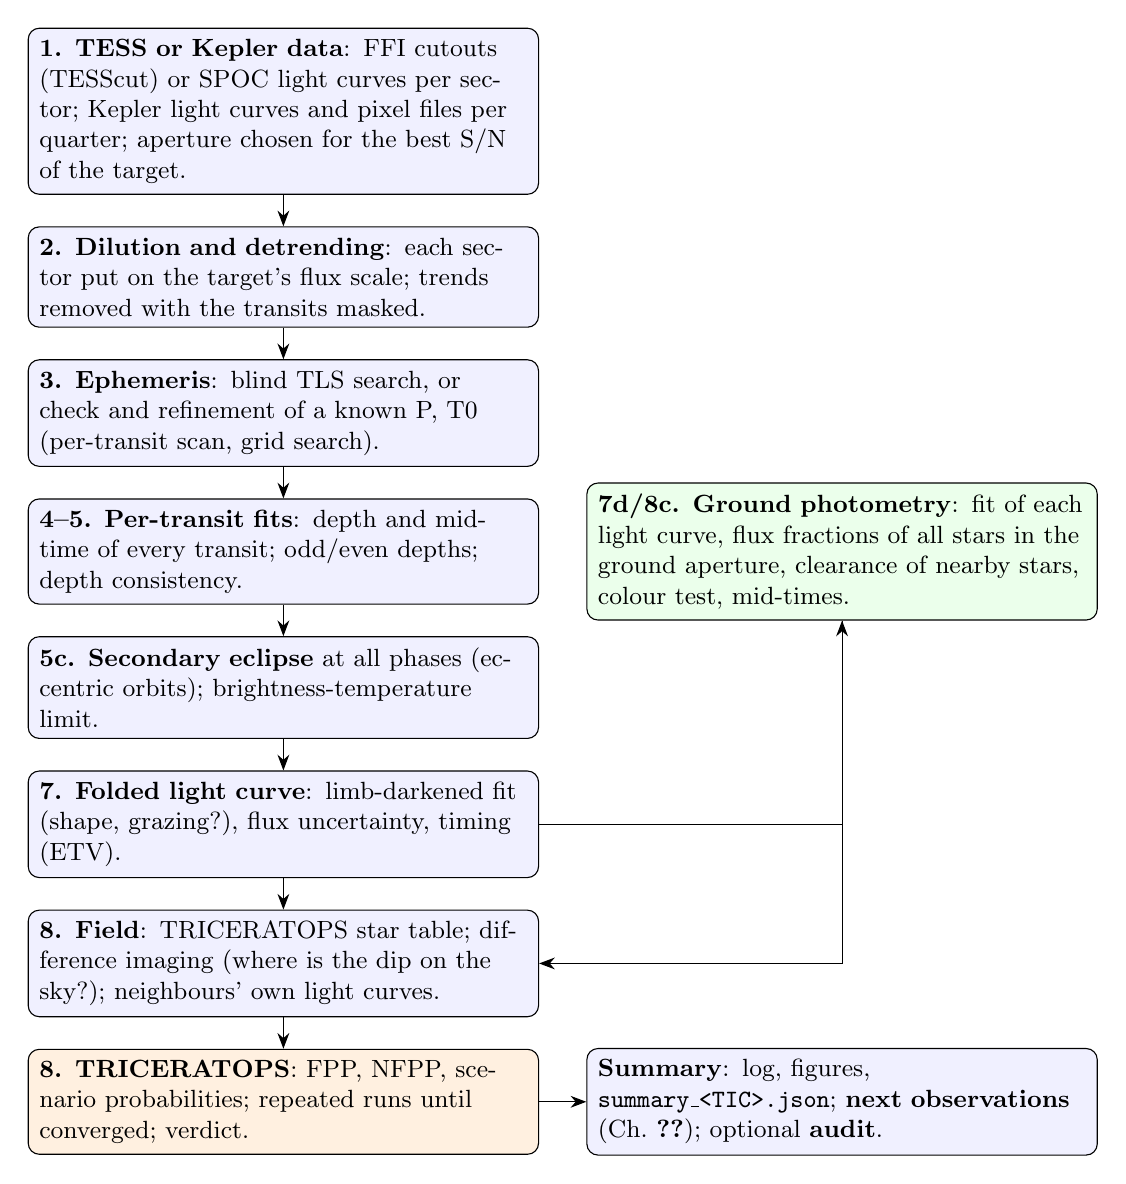
\begin{tikzpicture}[node distance=4mm and 6mm,
  box/.style={draw,rounded corners,fill=blue!6,align=left,font=\small,text width=6.2cm,inner sep=4pt},
  gbox/.style={draw,rounded corners,fill=green!8,align=left,font=\small,text width=6.2cm,inner sep=4pt},
  tbox/.style={draw,rounded corners,fill=orange!12,align=left,font=\small,text width=6.2cm,inner sep=4pt},
  arr/.style={-{Stealth[length=2mm]}}]
\node[box] (a) {\textbf{1. TESS or Kepler data}: FFI cutouts (TESScut) or SPOC light curves per sector; Kepler light curves and pixel files per quarter; aperture chosen for the best S/N of the target.};
\node[box,below=of a] (b) {\textbf{2. Dilution and detrending}: each sector put on the target's flux scale; trends removed with the transits masked.};
\node[box,below=of b] (c) {\textbf{3. Ephemeris}: blind TLS search, or check and refinement of a known P, T0 (per-transit scan, grid search).};
\node[box,below=of c] (d) {\textbf{4--5. Per-transit fits}: depth and mid-time of every transit; odd/even depths; depth consistency.};
\node[box,below=of d] (e) {\textbf{5c. Secondary eclipse} at all phases (eccentric orbits); brightness-temperature limit.};
\node[box,below=of e] (f) {\textbf{7. Folded light curve}: limb-darkened fit (shape, grazing?), flux uncertainty, timing (ETV).};
\node[gbox,right=of d] (g) {\textbf{7d/8c. Ground photometry}: fit of each light curve, flux fractions of all stars in the ground aperture, clearance of nearby stars, colour test, mid-times.};
\node[box,below=of f] (h) {\textbf{8. Field}: TRICERATOPS star table; difference imaging (where is the dip on the sky?); neighbours' own light curves.};
\node[tbox,below=of h] (i) {\textbf{8. TRICERATOPS}: FPP, NFPP, scenario probabilities; repeated runs until converged; verdict.};
\node[box,right=of i] (j) {\textbf{Summary}: log, figures, \texttt{summary\_<TIC>.json}; \textbf{next observations} (Ch.~\ref{ch:followup}); optional \textbf{audit}.};
\draw[arr] (a)--(b); \draw[arr] (b)--(c); \draw[arr] (c)--(d); \draw[arr] (d)--(e);
\draw[arr] (e)--(f); \draw[arr] (f)--(h); \draw[arr] (h)--(i); \draw[arr] (i)--(j);
\draw[arr] (f.east) -| (g.south);
\draw[arr] (g.south) |- (h.east);
\end{tikzpicture}
\end{center}

The diagnostic tests and what they reveal:

\begin{longtable}{@{}p{0.26\textwidth}p{0.67\textwidth}@{}}
\toprule
\textbf{Test} & \textbf{What a failure indicates}\\
\midrule\endhead
Odd/even depths & Different depths of alternating transits: an EB at twice the period.\\
Secondary eclipse & A dip elsewhere in the orbit: light from a self-luminous companion, so an EB. The limit gives a maximum temperature of the companion.\\
Limb-darkened fit & V shape, $b + k > 1$ (grazing), or a stellar density inconsistent with the star: EB or wrong host.\\
Difference imaging & The dip is centred on a neighbour instead of the target: NEB.\\
Neighbour vetting & A neighbour's own TESS light curve shows the dip more deeply.\\
Per-transit depths & Depths that differ between sectors: wrong dilution or a blend.\\
Timing (ETV) & Mid-time variations: a third body, or a wrong period.\\
Ground photometry & The dip on the ``wrong'' star, a wrong depth, or a colour-dependent depth (Chapter~\ref{ch:ground}).\\
\bottomrule
\end{longtable}

\section*{How the verdict is formed (v4.3)}
TRICERATOPS only sees the folded transit; it does not see the pipeline's own
tests. Since v4.3 the verdict therefore has two parts:
\begin{itemize}
\item \textbf{the criteria of Giacalone et al.\ (2021):} FPP $<0.015$ and
NFPP $<0.001$ (Chapter~2);
\item \textbf{the pipeline's own evidence against a planet at this period:}
a secondary eclipse that is too deep or too hot for a planet, odd and even
depths that differ by more than 3$\sigma$, or no transit at all at the odd
(or even) epochs, which means that the period is twice the input.
\end{itemize}
When the criteria are met but such evidence exists, the verdict is ``NOT
passed'' with the reason. A \emph{shallow, cool} secondary eclipse (less than
10\% of the transit depth and a brightness temperature below 4000~K) is
\emph{not} used against the planet: hot Jupiters such as WASP-18b show their
own occultation behind the star. The log then adds a note that a mass (radial
velocities) decides. \code{--no-eb-veto} switches this rule off.

Two other safeguards of v4.3 concern the depth and the ephemeris:
\begin{itemize}
\item the depth of the limb-darkened fit replaces the measured depth only when
the impact parameter $b$ is constrained and both depths agree within
3$\sigma$; otherwise the measured (per-transit) depth goes to TRICERATOPS;
\item a refined ephemeris is adopted only when it predicts every epoch with
data to better than a quarter of the transit duration; otherwise the folded
grid search decides.
\end{itemize}

%% ----------------------------------------------------------------------
\chapter{Ground-based observations in the analysis}
\label{ch:ground}

\section{The blending problem}

A TESS pixel is 21$''$ wide and the TESS point-spread function covers a few
pixels. Stars a few arcseconds apart are fully blended. In TIC~65344135 the
target ($V=12.98$) and its neighbour TIC~65344134 ($V=13.17$, at 5.9$''$) end
up in the same pixel (Figure~\ref{fig:blend}). TESS measures a dip of 3.2~ppt
in their combined light. If the target is the host, its own dip must be about
5.9~ppt; if the neighbour is the host, about 7.0~ppt. Under 2--3$''$ seeing a
ground-based telescope measures both stars separately and decides.

\begin{figure}[ht]
\centering
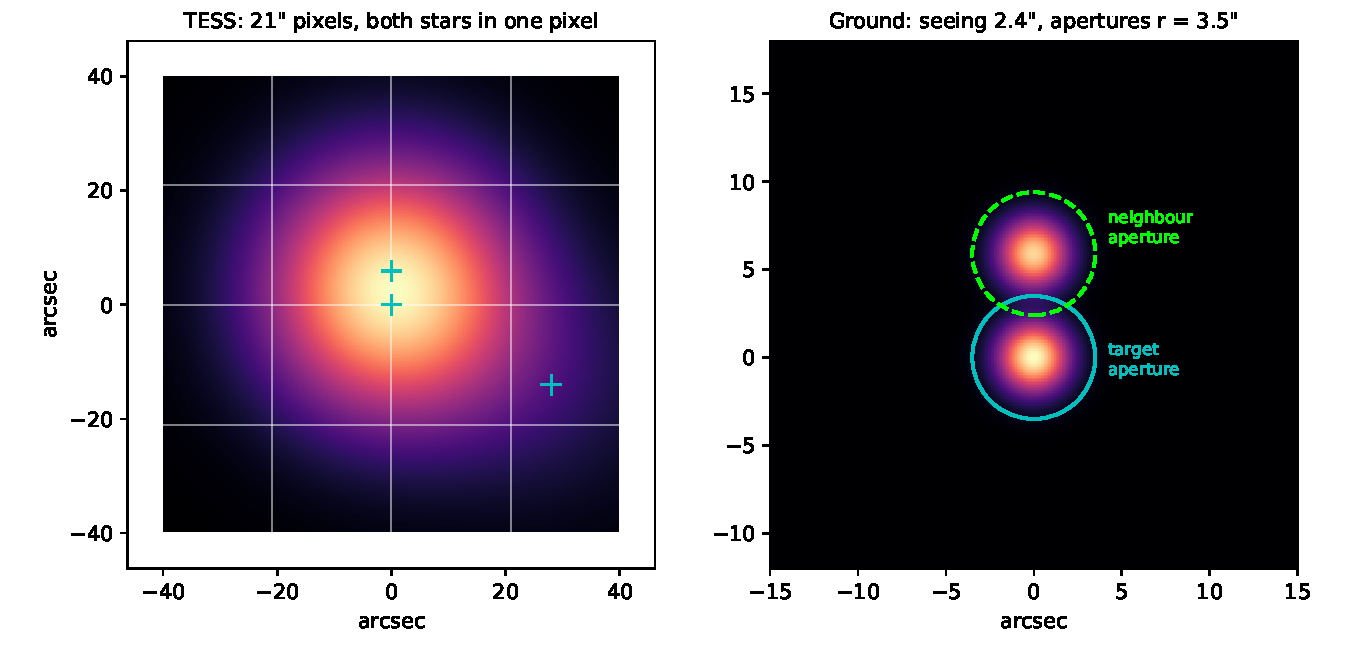
\includegraphics[width=\textwidth]{og_blend.pdf}
\caption{Simulated view of the field of TIC~65344135. Left: TESS, 21$''$
pixel grid; target and neighbour (crosses) fall in one pixel. Right: from the
ground with 2.4$''$ seeing, with apertures of 3.5$''$ radius on the target and
on the neighbour.}
\label{fig:blend}
\end{figure}

\section{What the pipeline does with a ground light curve}

\begin{enumerate}
\item \textbf{Fit.} The shape of the transit (duration, ingress and egress)
is taken from the TESS fit. Only the depth and the mid-time are free,
together with a baseline (linear in time, plus airmass when present). The
mid-time is searched within the uncertainty of the TESS ephemeris (at least
$\pm$60~min). The errors are inflated for correlated noise. Why the TESS
shape is used is explained in the box below.
\item \textbf{Flux fractions.} For every star near the target, the fraction
$\phi_j$ of the light in the ground aperture is computed. This uses the
aperture radius, the seeing and the magnitude of each star in the observed
band.
\item \textbf{Expected depth.} If star $j$ hosts the signal, its own
eclipse must have the depth $\delta_j$ that reproduces the TESS dip, and the
ground aperture must show $\phi_j\,\delta_j$.
\item \textbf{Clearance.} Star $j$ is \emph{excluded} when this expected dip
is absent ($\phi_j\delta_j$ well above the 3$\sigma$ upper limit), or when a
dip is seen that is much deeper than $\phi_j\delta_j$. Excluded neighbours are removed
before TRICERATOPS runs. The target is never removed, but if the ground data
contradict it, the log warns loudly.
\item \textbf{Colour.} The intrinsic depth is compared between bands and with
TESS. A planet's depth is almost the same in every band; an EB or blend often
is not.
\item \textbf{Timing.} Good mid-times are added to the ephemeris and ETV
analysis.
\end{enumerate}

\begin{tip}
\textbf{Why fit a ground light curve with the TESS shape?}
\begin{itemize}
\item \emph{The question is whether the TESS event is there.} The duration
and the ingress/egress times are set by the geometry of the orbit. They are
the same in every band and in every aperture; only the depth changes, with
the dilution and slightly with limb darkening. A dip of the right star must
therefore have the TESS shape.
\item \emph{TESS usually knows the shape much better.} The TESS template is
the fold of \emph{all} transits TESS observed (7 for TIC~65344135, more than
250 for WASP-18~b), each with baseline on both sides. A single ground light
curve has a few hours of data with trends from
airmass and seeing, often only one side of baseline, and an S/N of 5--15. A
free fit of duration and impact parameter to such data is badly degenerate
with the baseline. Fixing the shape leaves two well-determined numbers,
the depth and the mid-time. This holds when TESS has enough transits with
a good S/N; for a candidate with only one or two shallow TESS transits a
good ground light curve can define the shape better than TESS, and the
fit in \code{ground_lightcurves_<TIC>.pdf} shows whether the TESS template
still fits.
\item \emph{Depths must be comparable.} The clearance compares the ground
depth with the depth expected from TESS. That only works if both are
measured with the same template.
\item \emph{Non-detections need a template.} ``No dip'' becomes a number,
the 3$\sigma$ upper limit, only for a dip of a given shape and duration.
\end{itemize}
\textbf{Limitations.} Limb darkening is stronger in blue bands, so the bottom
of the transit is slightly more rounded there. This changes the fitted depth
by a few per cent, which the 25\% tolerance and the colour test absorb. A
dip with a clearly different duration would fit the template badly
($\chi^2$, residuals in \code{ground_lightcurves_<TIC>.pdf}). It would then
not be the TESS signal, or the TESS shape would be wrong. Either way, look
at the figure.
\end{tip}

\section{The output and how to read it: example TIC 65344135}
\label{sec:groundout}

A ground light curve leaves its traces in six places. They are explained
here with a synthetic test for TIC~65344135 (AAVSO campaign 942): one
transit observed three times, in Rc on the target, in $r'$ on the neighbour
TIC~65344134 (5.9$''$) and in B on the target, with 2~ppt per 1-min point.
The transit was injected on the target.

\begin{center}
\begin{tabular}{@{}p{0.42\textwidth}p{0.5\textwidth}@{}}
\toprule
Output & What it tells\\
\midrule
log, section \emph{Ground-based photometry} & fit of every light curve, flux fractions, verdict per star, colour test, TRICERATOPS+ use\\
\code{ground_lightcurves_<TIC>.pdf} & the data with the fitted transit (Section~\ref{sec:glcplot})\\
\code{ground_clearance_<TIC>.pdf}, \code{.csv} & which stars are consistent with, excluded by or not tested by each light curve (Section~\ref{sec:clearance})\\
\code{ground_chromaticity_<TIC>.pdf} & intrinsic depth per band (Section~\ref{sec:multiband})\\
\code{ground_times_<TIC>.txt} & mid-times for the ephemeris and timing analysis\\
\code{summary_<TIC>.json} (\code{ground}) and the audit & the results in one place; tests \emph{Ground data} and \emph{Multi-band}\\
\bottomrule
\end{tabular}
\end{center}

\subsection{The log}
For each light curve the log first gives the fit, then the apertures and
the verdicts. For the test:
\begin{lstlisting}
obsA_R_target: band R, aperture on target, 481 points, cadence 1.0 min, baseline poly1+AIRMASS
    epoch 23: predicted Tc = 2461348.24000 BJD_TDB +- 2.9 min
    coverage of the transit 100 % (baseline before: yes, after: yes); rms 2043 ppm, chi2_red 1.04, beta 1.00
    depth = 5844 +- 525 ppm (S/N 11.1); 3-sigma upper limit in the window 7419 ppm
    mid-time Tc = 2461348.24347 +- 2.0 min BJD_TDB (O - C = +5.0 min)
    DETECTED
obsB_r_neighbour: band r, aperture on TIC 65344134 ...
    depth = 317 +- 405 ppm (S/N 0.8); 3-sigma upper limit in the window 1937 ppm
    no significant dip
...
obsA_R_target [R]: aperture r = 3.5", FWHM 2.4"; flux fractions: 65344135 0.994, 65344134 0.006
combined verdict per star:  TIC 65344135 (target): consistent   TIC 65344134: excluded
intrinsic depth if TIC 65344135 is the host [ppm]: R: 5877 +- 557, B: 4970 +- 720; TESS 5900
    band-independent depth: chi2 = 1.6 for 2 dof, p = 0.455  -> achromatic
\end{lstlisting}
Read it in this order:
\begin{itemize}
\item \textbf{Coverage and baseline.} Was the whole transit window observed,
with baseline on both sides? A light curve that misses the window is
\emph{not usable} and tests nothing.
\item \textbf{Noise.} rms per point, $\chi^2_\nu$ near 1 and $\beta$ (red-noise
factor) near 1 mean that the errors are realistic; $\beta > 1.5$ means trends
that the baseline model did not remove.
\item \textbf{Depth and S/N.} ``DETECTED'' needs S/N $\geq$ 5 and a clear
improvement of the fit. Without a detection the \emph{3$\sigma$ upper limit}
is the useful number: it is what the clearance compares with. It is computed
as follows: the template is fitted at every trial mid-time in the search
window (only mid-times at which at least half of the transit is covered),
each fit gives a depth $A$ and its error $\sigma_A$ (inflated for red noise),
and the limit is the largest value of $A + 3\sigma_A$ over the window. A dip
deeper than that is excluded at 3$\sigma$ wherever in the window it falls.
\item \textbf{Mid-time.} O$-$C against the TESS ephemeris; a few minutes is
normal, much more than the window means the dip is probably not the TESS
event.
\item \textbf{Flux fractions, verdicts, colour, TRICERATOPS+:} explained in
the next sections.
\end{itemize}

\subsection{The fitted light curves}
\label{sec:glcplot}
\begin{figure}[ht]
\centering
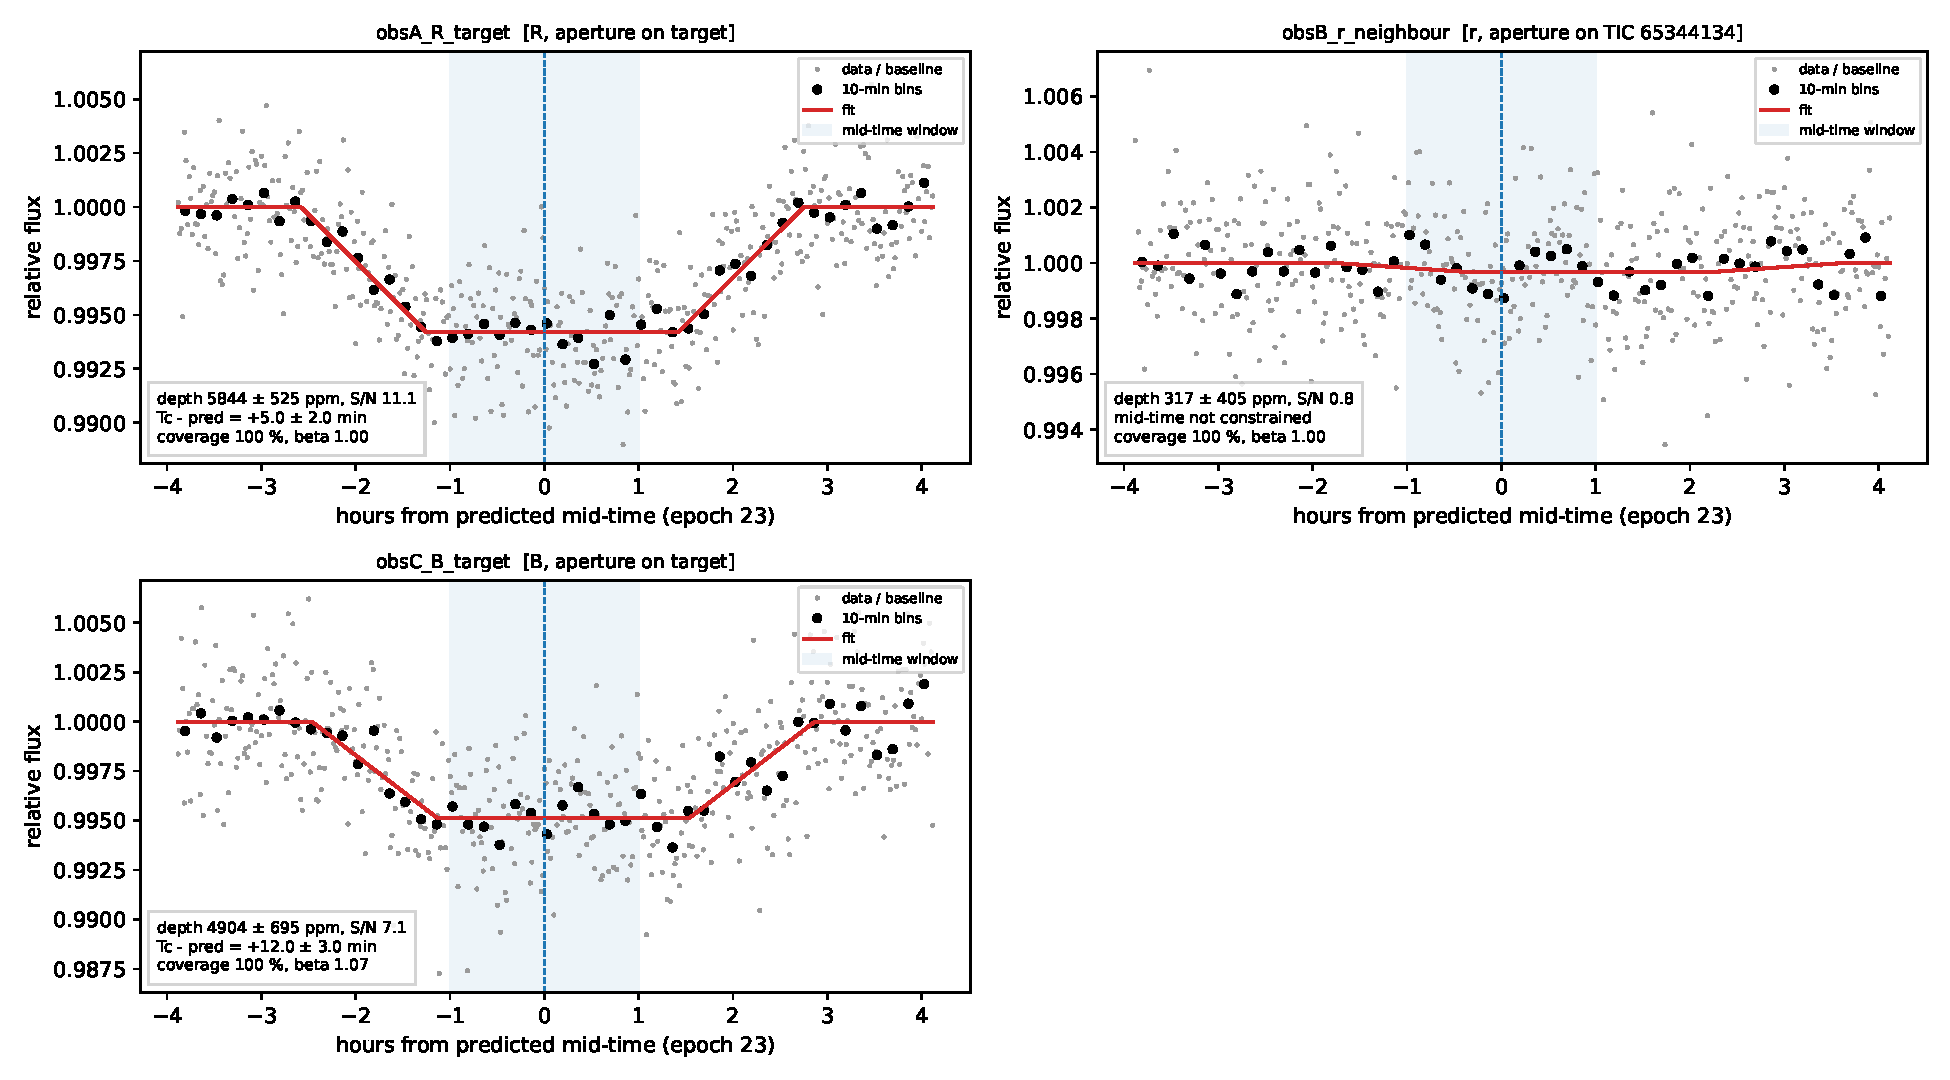
\includegraphics[width=0.95\textwidth]{ground_lightcurves_example.pdf}
\caption[Fitted ground light curves]{\code{ground_lightcurves_<TIC>.pdf} for the synthetic test of
TIC~65344135: Rc on the target (dip detected), $r'$ on the neighbour (no
dip), B on the target (dip detected). Shaded: the window in which the
mid-time is searched; dashed: the predicted mid-time.}
\label{fig:glc}
\end{figure}

One panel per light curve: the detrended data (points and 10-min bins) and
the fitted transit with the TESS shape; the box repeats depth, S/N, the
offset from the predicted mid-time, the coverage and $\beta$. Check that the
dip lies in the shaded window, that the bins follow the red curve without
systematic deviations (a dip of another duration would not fit the
template) and that the baseline is flat on both sides. In the test, the two target light curves show the transit; the
neighbour's aperture is flat within the noise.

\begin{figure}[p]
\centering
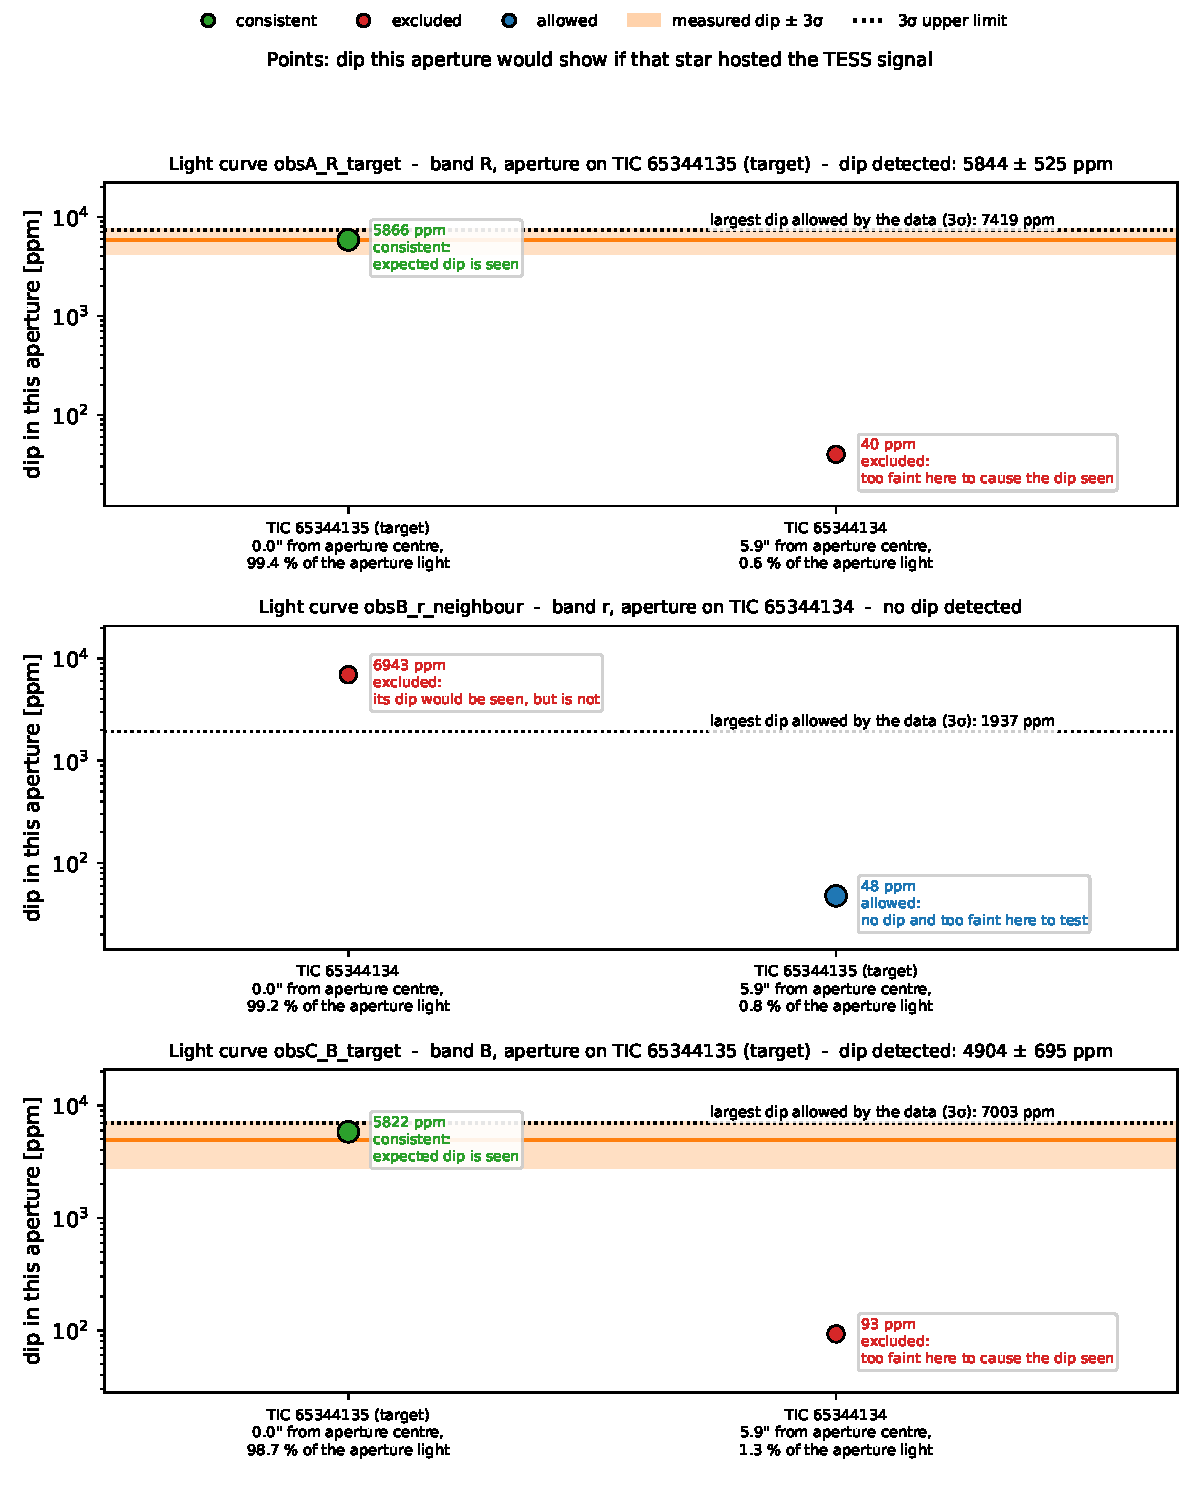
\includegraphics[width=0.93\textwidth]{ground_clearance_example.pdf}
\caption[Clearance diagram]{Clearance diagram (\code{ground_clearance_<TIC>.pdf}) for the three
synthetic light curves of Figure~\ref{fig:glc}. One panel per ground light
curve. Each point is a star that could host the TESS signal. Its height is
the dip \emph{this} aperture would show if that star were the host. The
orange band is the measured dip $\pm3\sigma$ (only when a dip is detected);
the dotted line is the largest dip the data allow. Colours: green
\emph{consistent}, red \emph{excluded}, blue \emph{allowed}, grey
\emph{unconstrained}. The reasoning is explained in the text.}
\label{fig:gclear}
\end{figure}

\subsection{The clearance diagram}
\label{sec:clearance}

\code{ground_clearance_<TIC>.pdf} (Figure~\ref{fig:gclear}), with the same
numbers in \code{ground_clearance_<TIC>.csv}.

The diagram answers one question per light curve and per star: \emph{if this
star were the source of the TESS dip, what would this ground aperture have
to show?} The steps below are general; the examples are the three light
curves of the synthetic test (TESS dip of 3.2~ppt; target and neighbour at
5.9$''$).

\begin{enumerate}
\item \textbf{The expected dip of each star.} TESS measures the dip $\delta_\mathrm{TESS}$
in the light of all stars in its aperture. For each star $j$ that could host
the signal, TRICERATOPS computes how deep that star's \emph{own} eclipse
$\delta_j$ would have to be to produce it: the fainter the star's share of
the TESS light, the deeper. In a ground aperture star $j$ contributes a
fraction $\phi_j$ of the light (printed under its name; it depends on the
aperture radius, the seeing, the band and the separation). If $j$ were the
host, the aperture would therefore show a dip of $\phi_j\,\delta_j$. This is
the height of the point.\\
\emph{Example:} the target would need $\delta \approx 5.9$~ppt, the
neighbour 6.9~ppt. In the target aperture (top panel) the target supplies
99.4\% of the light, $0.994 \times 5.9 \approx 5866$~ppm; the neighbour
0.6\%, $0.006 \times 6.9~\text{ppt} \approx 40$~ppm.
\item \textbf{What was measured.} The title of each panel says whether a dip
was detected. If it was, the orange line and band show its depth and
3$\sigma$ range. The dotted line is the 3$\sigma$ upper limit of
Section~4.3.1: the largest dip compatible with the data for any mid-time in
the search window.
\item \textbf{The verdict per star and per light curve:}
\begin{description}
\item[Consistent (green).] A dip is detected and the point lies in the
orange band: the dip this star would cause is the dip that is seen.
\emph{Example:} the target in the top and bottom panels.
\item[Excluded, ``its dip would be seen, but is not''.] The point lies
well above the dotted line: in this aperture the star would produce a dip
larger than the data allow. This is the test that clears a neighbour with
an aperture centred on it.
\emph{Example (middle panel):} in its own aperture the neighbour would cause
6943~ppm, at most 1937~ppm is allowed.
\item[Excluded, ``too faint here to cause the dip seen''.] A dip \emph{is}
detected, but it is deeper (beyond 3$\sigma$) than this star could cause
even as the host, because it supplies too little light to the aperture.
\emph{Example (top panel):} the neighbour could cause 40~ppm in the target
aperture, 5844~ppm is seen.
\item[Allowed (blue).] No conflict, but also no test: no dip is seen, and
the dip this star would cause \emph{in this aperture} is far below what the
data can detect. ``Too small'' refers to the star's share of the light in
this aperture, not to its brightness. The light curve neither supports nor
contradicts this star: it would look the same whether the star is the host
or not.
\emph{Example (middle panel):} the target, seen in the aperture on the
neighbour. It supplies only 0.8\% of the light there, so as the host it
would cause $0.008 \times 5.9~\text{ppt} \approx 48$~ppm. The light curve
measures $317 \pm 405$~ppm at the best-fitting mid-time and $289 \pm
511$~ppm at the predicted one (S/N 0.8): no dip is detected, and the 3$\sigma$
upper limit over the $\pm60$-min window is 1937~ppm. A dip of 48~ppm is
0.1$\sigma$ of this measurement, so the data cannot tell it from no dip at
all: what is seen is exactly what is expected if the target is the host,
but also if it is not. The target is tested by the light curves
centred on it (top and bottom panels), where it is \emph{consistent}.
\item[Unconstrained (grey).] The light curve does not cover the transit
window, so it says nothing.
\end{description}
\item \textbf{Combining the light curves.} A star excluded in at least one
light curve, and consistent in none, is removed before TRICERATOPS; its
NTP/NEB scenarios disappear. The target is never removed: if the ground
data exclude it, the log warns that the candidate is probably a false
positive. A star excluded in one light curve and consistent in another is
reported as a \emph{conflict} and kept; check the apertures, filters and
comparison stars.\\
\emph{Example:} the neighbour is excluded twice (top and middle panels), the
target is consistent twice (R and B): the neighbour is removed.
\end{enumerate}

A tolerance of 25\% on the expected depth (\code{--ground-depth-tol})
absorbs the uncertainties of the seeing model, the band magnitudes and limb
darkening. A star is never excluded on a difference smaller than that.


\subsection{Several filters: the colour test and TRICERATOPS+}
\label{sec:multiband}

\subsubsection*{Why colour helps}

A planet blocks the same fraction of the starlight in every band; only limb
darkening makes the depth differ by a few per cent between blue and red.
Most false positives do not have that property, because the star that is
eclipsed, or the star that dilutes the dip, has another colour than the
target:

\begin{center}
\begin{tabular}{@{}p{0.26\textwidth}p{0.66\textwidth}@{}}
\toprule
Scenario & Depth versus band\\
\midrule
TP, PTP, DTP (planet) & the same in every band (limb darkening: a few \%)\\
SEB, SEBx2P, STP & the dip is on a bound companion, diluted by the target:
deeper in the band where the companion is relatively brighter (red for a
cooler companion)\\
PEB, PEBx2P & the dip is on the target, diluted by a companion of another
colour: shallower where the companion is brighter\\
BEB, BEBx2P, BTP, DEB, DEBx2P & as above, for an unresolved background or
foreground star of unknown colour\\
NEB, NTP & a resolved neighbour: tested with separate apertures, not with
colours\\
EB, EBx2P & an eclipsing binary on the target: often nearly achromatic;
spectroscopy tests it\\
\bottomrule
\end{tabular}
\end{center}

The farther apart the two bands, the larger the effect: $g'$ with $z'$ (or B
with I) is far better than V with R.

\begin{figure}[ht]
\centering
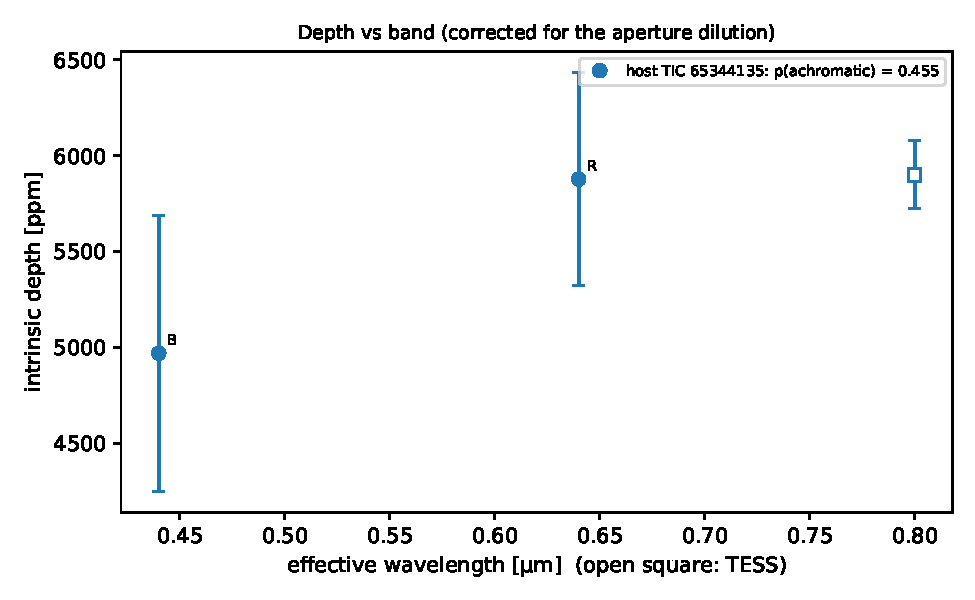
\includegraphics[width=0.62\textwidth]{ground_chromaticity_example.pdf}
\caption[Depth versus band]{\code{ground_chromaticity_<TIC>.pdf} for the synthetic test of
TIC~65344135: the measured depth in each band divided by the target's
flux fraction in that aperture, i.e.\ the intrinsic depth if the target is
the host (dots), and the TESS value (open square). B lies 1.2$\sigma$ below
Rc and TESS; all three agree within their errors ($\chi^2$ test,
$p = 0.46$; see the text).}
\label{fig:gchrom}
\end{figure}

\subsubsection*{Two ways the pipeline uses the bands}

\begin{enumerate}
\item \textbf{TRICERATOPS+.} The extended version of TRICERATOPS
(installed in the \code{triplus} environment) fits the ground light curves
together with TESS. For every scenario it predicts the light curve in each
band, with the band-dependent flux fractions of all stars
(\code{fluxratio_<band>}), and multiplies the likelihoods. The pipeline
passes at most seven light curves, \emph{one per band}: the most precise
usable light curve in each of $g$, $r$, $i$, $z$, $J$, $H$, $K$ (Rc and Ic
count as $r$ and $i$). B, V and clear-filter light curves are not
TRICERATOPS+ bands; they enter only the clearance and the colour test.
With TRICERATOPS+ the reported FPP \emph{already includes} the ground data.
With the original TRICERATOPS (option \code{--tri-plus off}, or another
environment) it does not.
\item \textbf{The colour test.} Independently of TRICERATOPS, the
pipeline converts every ground depth into the intrinsic depth of the host
(dividing by its flux fraction in that aperture and band) and compares the
bands with each other and with TESS (Figure~\ref{fig:gchrom}). Two numbers
summarise the comparison:
\begin{itemize}
\item \emph{$\chi^2$ and $p$.} With $d_k \pm \sigma_k$ the intrinsic depth
in band $k$ (one value per band; TESS included) and $\bar d$ their
error-weighted mean,
\[
\chi^2 = \sum_k \frac{(d_k - \bar d)^2}{\sigma_k^2},
\]
with $n-1$ degrees of freedom for $n$ bands. Each $\sigma_k$ includes a
3~\% systematic floor for the dilution model. The value $p$ is the
probability that a depth which is \emph{the same in every band} would give
a $\chi^2$ at least this large through noise alone (the tail of the $\chi^2$
distribution). A large $p$ means the depths are compatible with an
achromatic dip; the pipeline calls the dip \emph{chromatic} when
$p < 0.0027$, the probability of a 3$\sigma$ deviation. A large $p$ is not
a proof that the dip is achromatic: with large errors every depth
``fits''. That is what the second number is for.
\item \emph{Red/blue ratio.} The ratio of the depths in the reddest and the
bluest band, with its error. Three times that error is the smallest colour
difference these data could have detected.
\end{itemize}
When only one ground band is available, TESS serves as the second band.
\end{enumerate}

\textbf{Reading the example.} The intrinsic depth is $4970 \pm 720$~ppm in
B, $5877 \pm 557$~ppm in Rc and 5900~ppm in TESS. B is lower, but the same
depth was injected in both bands: the difference is noise (the B light
curve is noisier, 2.5 against 2~ppt per point, and its fitted mid-time is
12~min late). The test quantifies this: $\chi^2 = 1.6$ for 2 degrees of
freedom (three bands), $p = 0.46$: a depth that is the same in every band
gives a $\chi^2$ this large or larger in 46~\% of the cases, so it fits; and the ratio
red/blue $= 1.18 \pm 0.21$ is 0.9$\sigma$ from 1. The same number also
shows how weak this pair of light curves is as a colour test: a depth ratio
had to differ from 1 by more than about 60~\% (3$\sigma$) to be detected.
That excludes only strongly chromatic blends; the audit's \emph{Multi-band}
test states this limit (``a colour difference of more than \ldots{} would
have been seen'') and which scenarios it rules out.

\textbf{If the difference were real.} A blue depth significantly below the
red one means that the eclipsed object is redder (cooler) than the light
that dilutes it: for example a transit or eclipse on a cool companion or
background star, diluted by a hotter target (STP, SEB, BEB). A blue depth
above the red one points the other way: a dip on the target diluted by a
redder star. Before concluding either, check the things that also make a
depth depend on the band: comparison stars of very different colour, a
wrong filter name (and so a wrong flux fraction), and differential
extinction during the night. Limb darkening alone changes the depth by only
a few per cent.


\subsubsection*{What the audit says}

The audit test \emph{Multi-band} turns this into a short statement with
the numbers behind it:

\begin{description}
\item[NA] no ground light curves, or fewer than two bands with a measured
depth. The advice says which band to add.
\item[PASS] the depth is the same in every band within the stated limit,
as a planet on the target requires. The audit then lists the scenarios
whose best-fit companion predicts a colour difference the data exclude,
and those it cannot distinguish. Example from the test suite (bands $g$ and
$z$, original TRICERATOPS):
\begin{lstlisting}
PASS  Multi-band  the depth is the same in g and z within 6 % (3 sigma),
  as a planet on the target requires; triceratops is not TRICERATOPS+:
  the ground light curves did NOT enter the FPP; intrinsic depth
  z/g = 1.000 +/- 0.020; ruled out by the colours: SEBx2P (predicts 8.23,
  201 sigma off, P = 0.3); not distinguished: PEB (0.97); removing them
  gives FPP = 0.1429 (the reported FPP does not include the ground data)
  -> run with TRICERATOPS+ (--tri-plus on) so that the light curves
     enter the FPP itself
\end{lstlisting}
\item[WARN / FAIL] the depth depends on the band (more than 3$\sigma$ from
an achromatic depth): the dip is not a planet on the target, or the
dilution in one of the apertures is wrong. It is a FAIL when at least two
bands detect the transit with S/N $\geq 5$. The audit names the scenarios
whose companion reproduces the measured colour.
\end{description}

The page \emph{Next observations} of the audit uses the same calculation
before the observation: for every chromatic scenario it gives the expected
depth ratio between $g'$ and $z'$ and the depth error per band needed to
see it at 3$\sigma$ (Chapter~\ref{ch:followup}).

\subsubsection*{Planning a multi-band observation}

\begin{itemize}
\item \textbf{Bands far apart}, e.g.\ $g'$ and $z'$; simultaneous
observations (two telescopes, or a multi-channel camera) share the same
weather and systematics, which makes the ratio more robust.
\item \textbf{Precision.} A companion of similar colour changes the depth
by only a few per cent. The audit states the limit reached (``within
6~\%''); several transits per band combine.
\item \textbf{Same comparison stars and aperture} in all bands, and the
filter name in the file or in the specification (\code{band=z}); a
wrong filter name gives a wrong flux fraction and a false colour signal.
\item \textbf{Neighbours.} Colours do not replace separate apertures: a
nearby eclipsing binary is found with the clearance test, not with the
colour test.
\end{itemize}


\subsection{Mid-times}
Every light curve with a well-measured mid-time adds a line to
\code{ground_times_<TIC>.txt} (BJD\_TDB, error in minutes, label). These
times enter the timing analysis of the same run and can be passed to later
runs with \code{--extra-times}. A ground transit years after the TESS data
is the best way to refine the period. In the test:
\begin{lstlisting}
2461348.243472  2.00  obsA_R_target
2461348.248333  3.00  obsC_B_target
\end{lstlisting}

\subsection{In the summary and the audit}
\code{summary_<TIC>.json} collects everything under \code{ground}: per light
curve the band, depth, S/N, coverage and mid-time; the verdict per star; the
stars cleared; the colour test per host (depths per band, ratio of the
reddest to the bluest band with its error); and which light curves
TRICERATOPS+ used. The audit turns this into two tests:
\emph{Ground data} (do ground and TESS agree, which stars were cleared, any
conflict) and \emph{Multi-band} (Section~\ref{sec:multiband}). For the test
the verdict is: target consistent in Rc and B, neighbour excluded and
removed, depth achromatic; the neighbour's NTP/NEB scenarios disappear from
the FPP.



\section{Practical advice for observers}

\begin{itemize}
\item \textbf{Timing.} Observe the \emph{whole} transit with at least
45--60~min of baseline before ingress and after egress. Add the ephemeris
uncertainty (in the log, or ask) to the predicted times. The GUI tool
\emph{Predicted transit times} gives the next events
(Section~\ref{sec:tools}).
\item \textbf{Band.} A red band (Rc or Sloan $r'$) gives the best S/N for
most stars. A second band far from the first ($g'$ with $z'$, or B with I),
preferably at the same time, allows the colour test
(Section~\ref{sec:multiband}); only $g$, $r$, $i$, $z$, $J$, $H$, $K$ (and
Rc, Ic) enter TRICERATOPS+.
\item \textbf{Exposure.} Do not saturate. Cadences of 1--3~min are fine. The
transit of TIC~65344135 lasts 5.3~h, so binning loses nothing.
\item \textbf{Apertures.} Measure the target and \emph{each} neighbour that
could host the signal in separate apertures; in AstroImageJ, as targets T1,
T2, \ldots{} Choose a radius of about 1.5--2 times the seeing FWHM but
smaller than the separation, if possible. Report the radius and the FWHM in
arcseconds.
\item \textbf{Comparison stars.} Use several, of similar brightness and
colour; reject variables.
\item \textbf{Deliver raw relative fluxes.} Deliver them with an airmass
column, not a light curve you have already detrended: the pipeline fits the
baseline together with the transit.
\item \textbf{Times.} Use BJD\_TDB if possible. JD\_UTC is accepted and
converted, but say which one it is.
\item \textbf{Formats.} AstroImageJ measurement tables, AAVSO/EXOTIC
exoplanet reports or a simple table of time, flux and error are all read.
\item \textbf{Precision.} In the synthetic test, 2~ppt per 1-min point gave
the depth to $\pm0.5$~ppt. That is enough to tell 5.9~ppt from zero at more
than 10$\sigma$, and 5.9 from 7.0~ppt marginally. Several light curves
combine.
\end{itemize}

%% ----------------------------------------------------------------------
\chapter{Planning the follow-up: the audit and the next observations}
\label{ch:followup}

A run ends with an FPP and an NFPP, but the more useful question for an
observer is: \emph{which observation would change them most?} The pipeline
answers it at the end of every run, and the audit repeats the answer with its
own checks.

\section{The idea}
TRICERATOPS splits the probability over its scenarios (Chapter~2). The FPP is
the sum of the false-positive scenarios, and each kind of follow-up
observation can rule out a known group of them:

\begin{longtable}{@{}p{0.27\textwidth}p{0.3\textwidth}p{0.36\textwidth}@{}}
\toprule
\textbf{Observation} & \textbf{Scenarios it can remove} & \textbf{How}\\
\midrule\endhead
Ground photometry with a separate aperture on the target and on each nearby star & NTP, NEB, NEBx2P on stars wider than the seeing (\code{--ground-fwhm}, default 3$''$) & The star that shows the dip is the host. One good transit is enough.\\
High-resolution imaging (speckle, adaptive optics) & bound companions (PEB, PEBx2P, STP, SEB, SEBx2P), background stars (DEB, DEBx2P, BTP, BEB, BEBx2P), neighbours closer than the seeing & A contrast curve; it sees companions outside its inner working angle (\code{--hires-iwa}, default 0.1$''$).\\
Reconnaissance spectroscopy (2--3 epochs, $\sim$1~km\,s$^{-1}$) & EB and EBx2P on the target; bright bound companions & A stellar companion on the target gives a radial-velocity amplitude of km\,s$^{-1}$; a bright companion shows its own set of lines (SB2), also closer than imaging can resolve.\\
Transits in two or more filters & scenarios in which the dip comes from, or is diluted by, a star of another colour & A planet on the target has the same depth in every band.\\
\bottomrule
\end{longtable}

For every observation the pipeline computes what the FPP and NFPP would become
if the scenarios it addresses were ruled out:
\[
\mathrm{FPP}' = \frac{\sum_{\rm FP\ kept} p_i}{\sum_{\rm all\ kept} p_i},
\qquad
\mathrm{NFPP}' = \frac{\sum_{\rm NTP,NEB\ kept} p_i}{\sum_{\rm all\ kept} p_i},
\]
where $p_i$ are the pooled scenario probabilities of the run. It then
searches the shortest combination of observations that would bring FPP and
NFPP below the validation limits.

\section{Best case and typical outcome}
No observation removes everything it addresses. The guide therefore gives two
numbers per observation:
\begin{description}
\item[Best case:] every scenario the observation addresses is ruled out.
\item[Typical:] only the part an observation of that kind usually reaches:
\begin{itemize}
\item \emph{imaging}: the bound companions wider than the inner working angle.
With the separation distribution of Sun-like binaries (Raghavan et al.\ 2010)
and 0.1$''$ at 373~pc (37~au) that is about half of them; background stars:
95\%;
\item \emph{spectroscopy}: 70\% of the bright companions (their velocity can
coincide with that of the target);
\item \emph{multi-band transits}: the share of possible companions whose
colour differs enough to change the depth by more than 20\% between the two
filters (below); background stars, whose colour is unknown: 50\%;
\item \emph{ground photometry}: all of the resolved neighbours.
\end{itemize}
\end{description}
These typical fractions are reasonable assumptions, not measurements. They
rank the observations; they do not predict their outcome. And an observation
can also \emph{find} a false positive: if the ground light curve shows the dip
on the neighbour, the candidate is a nearby eclipsing binary, whatever the
numbers said.

\section{The colour test in detail}
If the dip comes from star X and is diluted by star Y, the observed depth in a
band is the true depth times the share of X in the light of that band:
\[
\delta_{\rm band} = \delta_X \,\frac{F_{X,{\rm band}}}{F_{X,{\rm band}} + F_{Y,{\rm band}}} .
\]
The share changes with the band when X and Y have different temperatures.
The pipeline approximates both stars by blackbodies (g$'$ at 0.48~$\mu$m,
z$'$ at 0.91~$\mu$m, TESS at 0.80~$\mu$m) and estimates the temperature of a
companion from its mass with a main-sequence relation
($T_{\rm eff} \approx 5772~{\rm K}\,(M/M_\odot)^{0.6}$):
\begin{itemize}
\item \textbf{STP, SEB} (dip on the companion): a redder companion makes the
dip deeper in z$'$ than in g$'$ (ratio below 1);
\item \textbf{PEB} (dip on the target, diluted by the companion): only a small
effect, a few percent;
\item \textbf{planet on the target}: ratio 1, apart from limb darkening.
\end{itemize}
How large the effect is depends on the companion, which the TESS data hardly
constrain. The pipeline therefore runs over all possible companions (mass
ratio 0.1--1, flat distribution), keeps those bright enough to produce the dip
at all (for STP a planet of at most two Jupiter radii, for SEB an eclipse of at
most 100\%), and counts the share that changes the depth by more than 20\%.
The best fit of the last TRICERATOPS run is shown as an example together with
the precision that a band test would need (three times the depth error must
fit in the depth difference).

\section{Companions that Gaia already excludes: MOLUSC}
\label{sec:molusc}

\subsection*{Why}
Several false-positive scenarios of TRICERATOPS need an unresolved
\emph{bound companion} of the target: PTP and PEB (the companion dilutes
the dip), STP and SEB (the dip is on the companion). Without other
information TRICERATOPS uses a general prior: how often stars of this mass
have a companion, and with which masses and separations (Moe \& Di~Stefano
2017). For many nearby stars that prior is too pessimistic: Gaia has
observed them for years, and a bright companion at the right distance would
have shown up. MOLUSC (\emph{Multi-Observational Limits on Unseen Stellar
Companions}, Wood, Mann \& Kraus 2021, AJ~162, 128) turns those
non-detections into a list of the companions that are still allowed. It
costs no telescope time.

\subsection*{How MOLUSC works}
\begin{enumerate}
\item \textbf{Simulate.} It draws a large number of companions (typically
$10^6$) for the target: mass ratio $q$ uniform between 0 and 1, a log-normal
period distribution (Raghavan et al.\ 2010), and random eccentricity,
inclination, orientation and orbital phase. Each simulated star has
exactly \emph{one} companion.
\item \textbf{Predict what each companion would have done}, with the
stellar models of Baraffe et al.\ (2015) for its brightness:
\begin{itemize}
\item \emph{Gaia astrometry (RUWE).} A companion at roughly 0.1--1$''$
makes the photocentre wobble and raises the RUWE (renormalised unit weight
error) of the Gaia solution. MOLUSC predicts the RUWE for every simulated
companion and rejects those whose prediction is clearly larger than the
observed value.
\item \emph{Gaia imaging.} A companion bright enough and far enough from the
star (beyond about 1$''$) would be a separate Gaia source.
\item \emph{Optional:} a high-resolution contrast curve (speckle, AO) and
radial-velocity measurements. With RVs, close companions (a few au and
less) can be excluded as well.
\end{itemize}
\item \textbf{Keep the survivors.} The file \code{<prefix>_kept.csv} lists
the companions that none of the data would have seen.
\end{enumerate}
The rejections are probabilistic (a companion is rejected with the
probability that it would have been detected), so a run with $10^6$
companions gives smooth distributions.

\subsection*{How the pipeline uses it}
\begin{enumerate}
\item \textbf{Run MOLUSC.} A copy with a few small fixes (newer SciPy/NumPy, a VizieR fallback) is
in the folder \code{MOLUSC} (see \code{README_pipeline.txt}). For each target a
short script gives the coordinates and the mass, e.g.\ for L~279-94:
\begin{lstlisting}
bash MOLUSC/run_molusc_L27994.sh       # in WSL, about 10 min
# -> TIC100796276_molusc/L27994_N1000000_kept.csv
\end{lstlisting}
MOLUSC needs the Gaia archive; when it does not answer (for instance while
it is closed for the DR4 release), the same Gaia DR3 values are read from
VizieR.
\item \textbf{Give the file to the pipeline:} GUI tab \emph{Field},
``MOLUSC companions file'' (\code{--molusc-file}) and ``MOLUSC: companions
generated'' (\code{--molusc-n}, the number MOLUSC simulated).
\item \textbf{What happens inside.} TRICERATOPS(+) takes the mass ratios of
the MOLUSC companions for the first draws of the PTP, PEB, STP and SEB
scenarios, and treats the remaining draws as ``no companion''. Two details
matter:
\begin{itemize}
\item It keeps only companions whose orbit never comes closer than 10~au to
the star (periastron $a(1-e) > 10$~au). Planets are rare in such close
binaries (Moe \& Kratter 2021), so TRICERATOPS assumes they do not exist
there.
\item The prior probability of a companion then becomes (number of
companions in the file)/(number of TRICERATOPS draws, $10^6$). Used as is,
the FPP would depend on how many companions one happened to simulate in
MOLUSC, and a file with more than $10^6$ survivors would crash
TRICERATOPS. The pipeline therefore resamples the survivors so that this
probability equals the MOLUSC survival fraction times an assumed
multiplicity (\code{--molusc-multiplicity}, default 1: every star has a
companion, the conservative choice).
\end{itemize}
The log lists the numbers: companions generated, kept, kept beyond 10~au,
the resulting prior, and their mass-ratio distribution. The audit names
the companion prior that was used (\emph{Evaluation}).
\end{enumerate}

\subsection*{Limitations}
\begin{itemize}
\item \textbf{It removes only what Gaia could have seen.} Companions very
close to the star (periastron $\lesssim$1~au) hardly change the RUWE and are
not resolved; without RV data they all survive. That they do not count in
the FPP is the \emph{assumption} that planets avoid close binaries, not a
measurement. A result that relies on MOLUSC should say so, and spectroscopy
(RVs or a second set of lines) is the observation that tests it.
\item \textbf{The RUWE is not only a binary indicator.} Variability, a
nearby source or a poor fit also raise it; a high RUWE makes MOLUSC reject
\emph{fewer} companions, which is safe. A RUWE that is low by chance would
make it reject too many.
\item \textbf{Models and distributions.} The companion population
(Raghavan), the stellar models (BHAC15, default age 5~Gyr) and the RUWE
calibration of the MOLUSC tables are assumptions; for very young or
evolved stars they matter.
\item \textbf{One companion per star.} Triples are not simulated. The
multiplicity (fraction of stars that have a companion at all) is not part
of MOLUSC; the pipeline uses 1 unless told otherwise, which overestimates
the companion probability (about a quarter of M dwarfs have one,
Winters et al.\ 2019).
\item \textbf{Different versions, different answers.} TRICERATOPS 1.1.0
treats the MOLUSC companions differently from the TRICERATOPS+ version
used here; the Zenodo note on L~279-94 obtains FPPs between 0.003 and 0.042
depending on such choices. Report the FPP with the companion model.
\item \textbf{Not a replacement for high-resolution imaging.} MOLUSC shows
that the companions which would invalidate the planet are \emph{unlikely};
an image or RVs show whether one is \emph{there}.
\end{itemize}


\section{Where to find it}
\begin{itemize}
\item at the end of the log, section \emph{Next observations};
\item in \code{recommendations_<tic>.txt} and in \code{summary_<tic>.json}
(\code{recommendations});
\item on the page \emph{Next observations} of the audit report
(Figure~\ref{fig:audit-next}), together with the advice of the audit's own
tests.
\end{itemize}

\section{The audit}
\code{triceratops_audit.py} reads an output folder and tries to break the
claim of the run, with deterministic checks only (no language model). The GUI
starts it with the button \emph{Audit run} on the tab \emph{Results} or from
the menu \emph{Tools}; it writes \code{audit_<tic>.pdf}, \code{.txt} and
\code{.json} and opens the PDF. The input files are never changed.

The report has four parts:
\begin{enumerate}
\item \textbf{Skeptic}: 17 tests with PASS, WARN, FAIL or NA, each with its
evidence, the file and line it comes from, and an advice (ephemeris,
single events, depth consistency, odd/even, secondary eclipse, shape and
density, dilution, centroids, neighbours, Monte-Carlo convergence,
sensitivity, ground data, multi-band colours and TRICERATOPS+
(Section~\ref{sec:multiband}), provenance of the input depth, and two
independent recomputations from the saved light curves, which leave out the
sectors the pipeline excluded and the transits of masked candidates);
\item \textbf{Next observations} (this chapter);
\item \textbf{Evaluation}: every claim of the run with its source;
\item \textbf{Recomputation}: the audit's own fold and per-sector depths.
\end{enumerate}
A FAIL does not change the pipeline's verdict; it marks a claim that needs a
closer look before the result is reported.

\begin{figure}[p]
\centering
\includegraphics[page=3,height=0.86\textheight,trim=0 25mm 0 0,clip]{audit_65344135.pdf}
\caption{Audit of TIC~65344135 (run of 12~November 2026), page \emph{Next
observations}. Ground photometry with separate apertures removes the
neighbour (FPP $0.391 \rightarrow 0.026$); spectroscopy or a colour test then
removes most of the rest.}
\label{fig:audit-next}
\end{figure}


%% ======================================================================
\part{Using the GUI}
%% ======================================================================

\chapter{Installation and start}

\section{What you need}

\begin{description}
\item[The scripts.] \code{triceratops_validation.py}, \code{triceratops_gui.py},
the folders \code{profiles/} and \code{tests/}, all in one folder, here
\code{D:\\EXPLORE\\candidates_dymock} (in WSL:
\code{/mnt/d/EXPLORE/candidates_dymock}).
\item[A Python environment for the pipeline.] It needs triceratops 1.1,
lightkurve, astroquery, wotan, transitleastsquares, numpy, scipy and
matplotlib. Optionally, a second environment \code{triplus} holds
TRICERATOPS+ (technical manual, Chapter~52):
\begin{lstlisting}
conda create -n triplus -c conda-forge python=3.11 "numpy<2.4" scipy pandas matplotlib astropy astroquery numba celerite emcee seaborn arviz corner pytest
conda activate triplus
pip install lightkurve "pytransit==2.2.0" mechanicalsoup pyrr wotan transitleastsquares "setuptools<81"
git clone https://github.com/JGB276/TRICERATOPS-plus.git
cd TRICERATOPS-plus && pip install .
\end{lstlisting}
\item[Tkinter for the GUI.] Any conda Python has it. A system Python on
Ubuntu/WSL needs \code{sudo apt install python3-tk}. On Windows 11 the GUI
window of WSL appears on the desktop automatically (WSLg).
\end{description}

\section{Starting}

\begin{lstlisting}
cd /mnt/d/EXPLORE/candidates_dymock
python triceratops_gui.py
\end{lstlisting}
The GUI reads the options from the validation script in the same folder and
restores your last session. Check the installation once with
\emph{Tools $\rightarrow$ Run regression tests}; all tests should pass.

%% ----------------------------------------------------------------------
\chapter{A tour of the window}

\begin{figure}[ht]
\centering
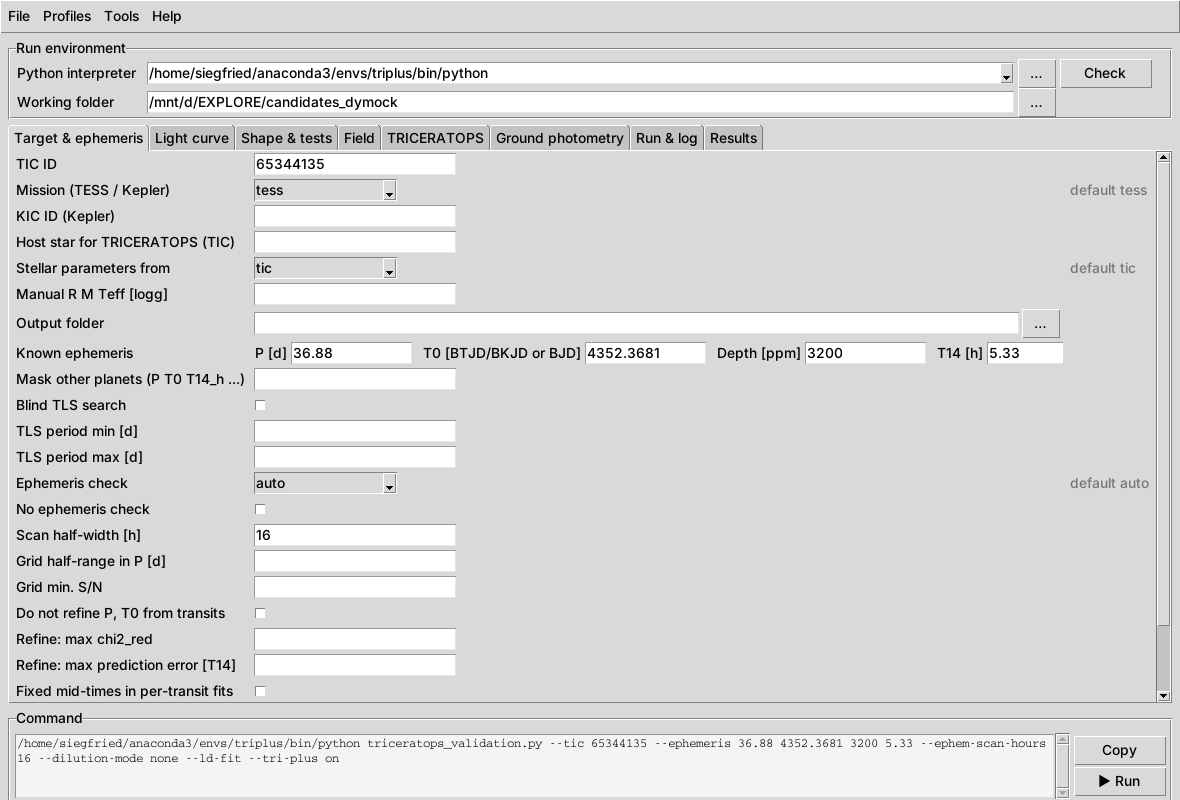
\includegraphics[width=\textwidth]{og_tab_target.png}
\caption{The main window (GUI v1.2) with the TRICERATOPS+ profile of TIC~65344135 loaded. New in v1.2 on this tab: \emph{Mission}, \emph{KIC ID}, \emph{Host star}, \emph{Stellar parameters from}, \emph{Manual R M Teff} and \emph{Mask other planets}.}
\label{fig:main}
\end{figure}

From top to bottom (Figure~\ref{fig:main}):
\begin{description}
\item[Menu bar.] \emph{File} (profiles, import or copy a command),
\emph{Profiles} (ready-made settings per object), \emph{Tools} (interpreter
check, transit times, tests, \emph{Audit output folder}), \emph{Help} (this
manual and the technical one, command-line help).
\item[Run environment.] The \emph{Python interpreter} that runs the
pipeline. Choose your triceratops~1.1 environment, or \code{triplus} for
TRICERATOPS+. \emph{Check} shows which triceratops it contains. The
\emph{Working folder} is where the run starts; results go to
\code{TIC<tic>/} in this folder unless an output folder is set.
\item[Tabs.] Six tabs with options, then \emph{Run \& log} and
\emph{Results} (with the button \emph{Audit run}). Hover over an option's name to see its command-line flag and
explanation. Grey text on the right shows the default. Empty fields mean
``use the default''.
\item[Command.] The exact command that will run, updated as you type. Red
text below it explains what is missing or inconsistent. \emph{Copy} puts it
on the clipboard, for a terminal or for your notes.
\end{description}

\textbf{New fields in v1.2.} On the tab \emph{Target \& ephemeris}:
\begin{description}
\item[Mission, KIC ID.] \emph{kepler} with a KIC number analyses Kepler data
(Chapter~\ref{ch:kepler}); the TIC field may then stay empty.
\item[Host star for TRICERATOPS.] TRICERATOPS treats this TIC star as the host,
for example a close companion, while the light curve stays that of the
target. The light curve is then used on the aperture scale (SAP, no dilution
correction).
\item[Stellar parameters from, Manual R M Teff.] Radius, mass and temperature
of the host from the TIC (default), from the Kepler catalogues (Berger et
al.\ 2020, else the DR25 table), or typed in, e.g.\ from a paper.
\item[Mask other planets.] P, T0 and T14 of other planets in the system; their
transits are removed from the light curve (e.g.\ TOI-7930.01 when analysing
.02).
\end{description}
On the tab \emph{TRICERATOPS}: \emph{Verdict from FPP/NFPP only} (switch off
the pipeline's own EB evidence, Chapter~\ref{ch:pipeline}) and \emph{Imaging
inner working angle}, used for the recommended next observations.

\section{Profiles}

A \emph{profile} holds all the settings for one object. The menu
\emph{Profiles} (Figure~\ref{fig:prof}) lists the profiles in the folder
\code{profiles/}. Choosing one replaces all options: options not in the
profile return to their defaults, so the same profile always gives the same
command. The supplied profiles:

\begin{longtable}{@{}p{0.34\textwidth}p{0.59\textwidth}@{}}
\toprule
\textbf{Profile} & \textbf{Object and settings}\\
\midrule\endhead
\code{profile_TIC65344135} & AAVSO campaign 942, triceratops 1.1: P = 36.88~d, T0 = BTJD 4352.3681, 5900~ppm (on the target's scale), T14 = 5.33~h, scan $\pm$16~h, LD fit.\\
\code{profile_TIC65344135_triplus} & The same for the \code{triplus} environment (TRICERATOPS+): 3200~ppm (aperture scale), dilution correction none, TRICERATOPS+ on.\\
\code{profile_TIC229788204} & Grazing EB candidate, P = 93.83471~d; LD fit, sensitivity runs.\\
\code{profile_TIC165501544} & P = 132.42~d, 3228~ppm; grid search.\\
\code{profile_TIC229675482} & P = 145.841~d, 863~ppm; grid search.\\
\code{profile_TIC229701403_b}, \code{_c} & Two long-period candidates, separate output folders.\\
\code{profile_template_new_candidate} & Start for a new object.\\
\bottomrule
\end{longtable}

Save your own with \emph{File $\rightarrow$ Save profile}, which also stores
the interpreter and working folder, or \emph{Save target profile (options
only)}, the version to pass on to colleagues. You are asked for a short
description, shown in the menu.

\begin{figure}[ht]
\centering
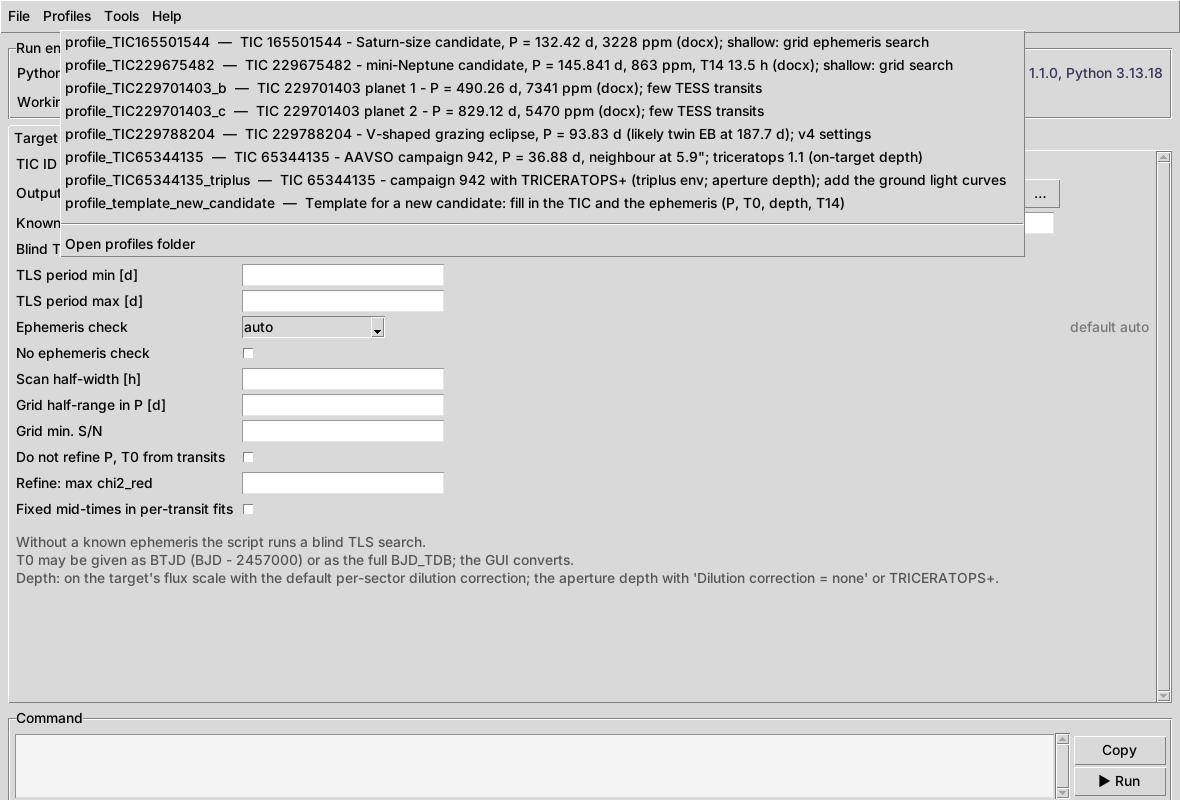
\includegraphics[width=0.9\textwidth]{og_profiles_menu.png}
\caption{The \emph{Profiles} menu.}
\label{fig:prof}
\end{figure}

%% ----------------------------------------------------------------------
\chapter{Worked example: AAVSO campaign 942 (TIC 65344135)}
\label{ch:example}

\textbf{Situation.} TESS shows six transits of 3.2~ppt with P = 36.88~d.
The neighbour at 5.9$''$ could be the source. Dennis Conti's campaign asks for
ground photometry of the transits of 7~November and 14~December 2026, with
target and neighbour measured separately, in a red and if possible a blue
band.

\section*{Step 1 --- Load the profile and check the environment}
\begin{enumerate}
\item \emph{Profiles $\rightarrow$ profile\_TIC65344135}. For TRICERATOPS+
choose \code{profile_TIC65344135_triplus} instead.
\item Choose the matching interpreter and press \emph{Check}. The text next
to it reads, for example, ``triceratops 1.1.0, Python 3.13'' or
``TRICERATOPS+ 1.0.17, Python 3.11''.
\item Look at the tab \emph{Target \& ephemeris} (Figure~\ref{fig:main}).
The ephemeris fields hold P, T0, depth and T14. T0 may be typed as the full
BJD from the campaign page (2461352.3681); the GUI converts it to BTJD and
says so under the command.
\end{enumerate}

\section*{Step 2 --- Plan the observation (optional)}
\label{sec:tools}
\emph{Tools $\rightarrow$ Predicted transit times} lists the next transits
from the ephemeris fields (Figure~\ref{fig:transits}). The UTC times are
approximate ($\pm$8~min, no barycentric correction); for 7~November the tool
gives 20:48~UTC, the campaign page 20:43~UTC. Add the ephemeris uncertainty
and the baseline before and after.

\begin{figure}[ht]
\centering
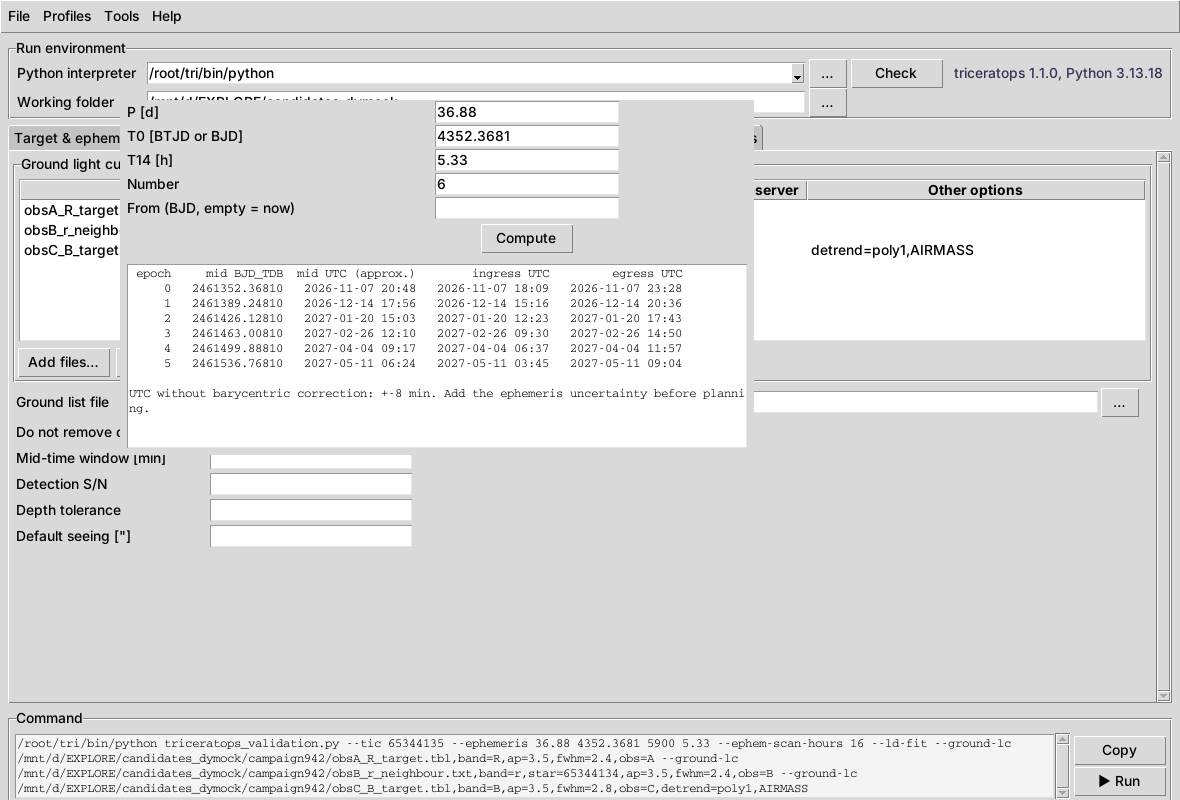
\includegraphics[width=0.95\textwidth]{og_transits.png}
\caption{Predicted transits of TIC~65344135.}
\label{fig:transits}
\end{figure}

\section*{Step 3 --- Add the ground light curves}
Put the observers' files in a subfolder, for example \code{campaign942/}.
On the tab \emph{Ground photometry} (Figure~\ref{fig:gtab}) press \emph{Add
files}, select one or more files and fill in the dialog for each
(Figure~\ref{fig:gdlg}):

\begin{longtable}{@{}p{0.24\textwidth}p{0.69\textwidth}@{}}
\toprule
\textbf{Field} & \textbf{What to enter}\\
\midrule\endhead
Band & R (= Rc), V, B, I, or Sloan g r i z; also J H K, CBB, clear. Empty: from the file header, else R.\\
Aperture star (TIC) & Empty for the target; 65344134 for the neighbour's aperture.\\
Aperture radius & Radius in arcsec, as used in the photometry.\\
Seeing FWHM & In arcsec (median of the night).\\
Observer & Name or AAVSO code.\\
Time system & Empty or BJD\_TDB; JD\_UTC or HJD\_UTC if that is what the file has.\\
Flux / error / time column & Only if the defaults are not right, e.g.\ \code{rel_flux_T2} for the neighbour in an AstroImageJ table where it is T2.\\
Magnitudes & 1 if the flux column holds magnitudes.\\
Detrend & Empty (= linear + airmass); \code{poly2} or extra columns, e.g.\ \code{poly1,AIRMASS,FWHM_Mean}.\\
Centre RA/Dec, pixel scale & Rarely needed (aperture not on a catalogued star; AstroImageJ radii in pixels).\\
TRICERATOPS+ band & Only to override the automatic choice.\\
\bottomrule
\end{longtable}

The same AstroImageJ file can be added twice, once for the target (T1) and
once for the neighbour (\code{fcol=rel_flux_T2}, aperture star 65344134).
\emph{Save as list} writes the table to a list file that can be used on the
command line (\code{--ground-list}); \emph{Import list} reads one.

\begin{figure}[ht]
\centering
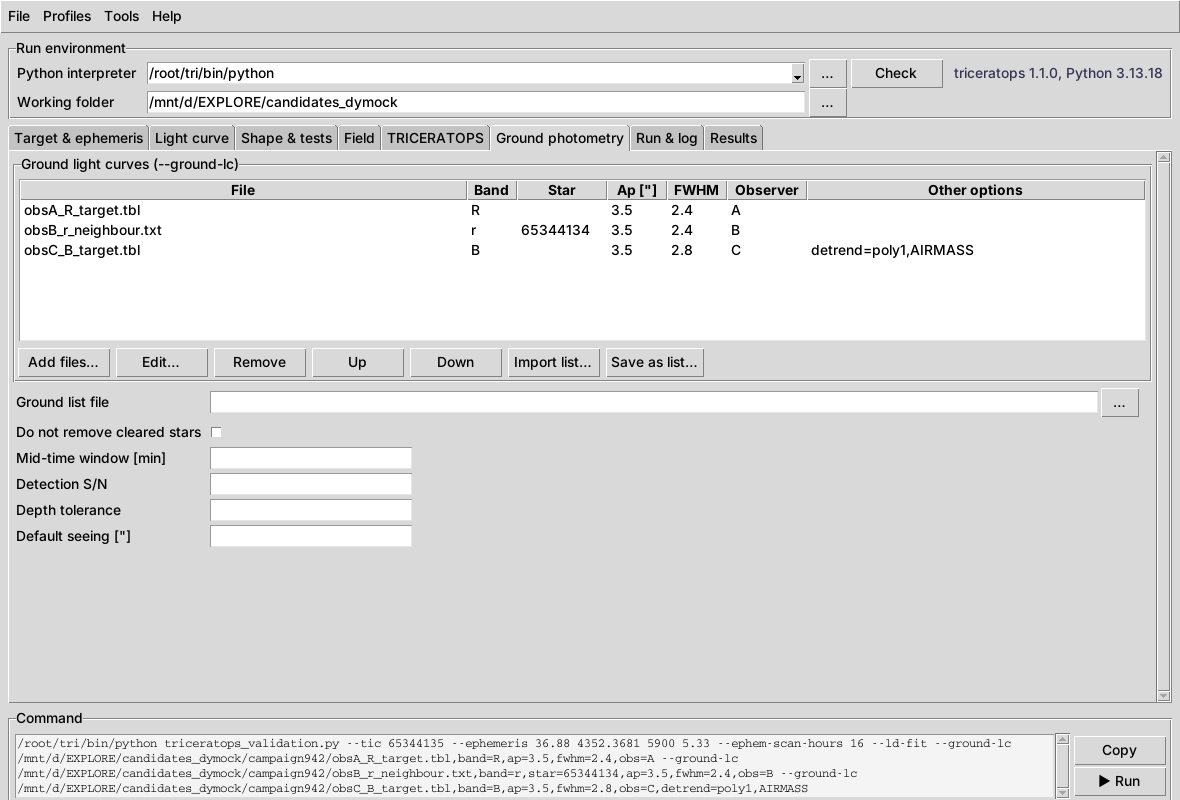
\includegraphics[width=\textwidth]{og_tab_ground.png}
\caption{Tab \emph{Ground photometry} with three light curves.}
\label{fig:gtab}
\end{figure}

\begin{figure}[ht]
\centering
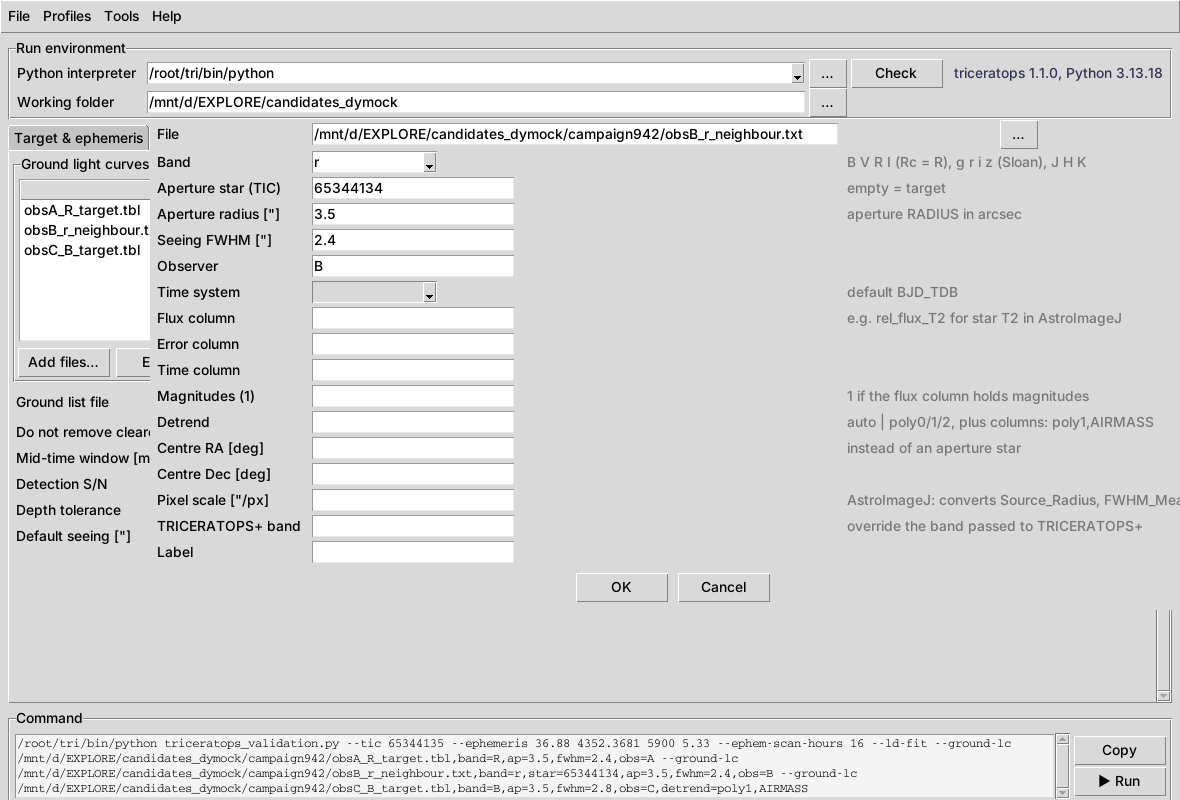
\includegraphics[width=\textwidth]{og_ground_dialog.png}
\caption{The dialog for one ground light curve (the neighbour's aperture).}
\label{fig:gdlg}
\end{figure}

\section*{Step 4 --- Save, run and follow}
\begin{enumerate}
\item \emph{File $\rightarrow$ Save profile} keeps this set-up, for example as
\code{profile_TIC65344135_campaign.json}.
\item Press \emph{Run}. The tab \emph{Run \& log} shows the output as it
comes (Figure~\ref{fig:run}): section headers in blue, warnings in red. The
status line shows the elapsed time and the current step.
\item Typical durations:
\begin{itemize}
\item the first download of all TESScut sectors: tens of minutes; later runs
use the cache;
\item the light-curve analysis: a few minutes;
\item the TRICERATOPS runs: up to the time budget, 1~h by default.
\end{itemize}
\item \emph{Stop} ends a run. You can close the window only after
confirming.
\end{enumerate}

\begin{figure}[ht]
\centering
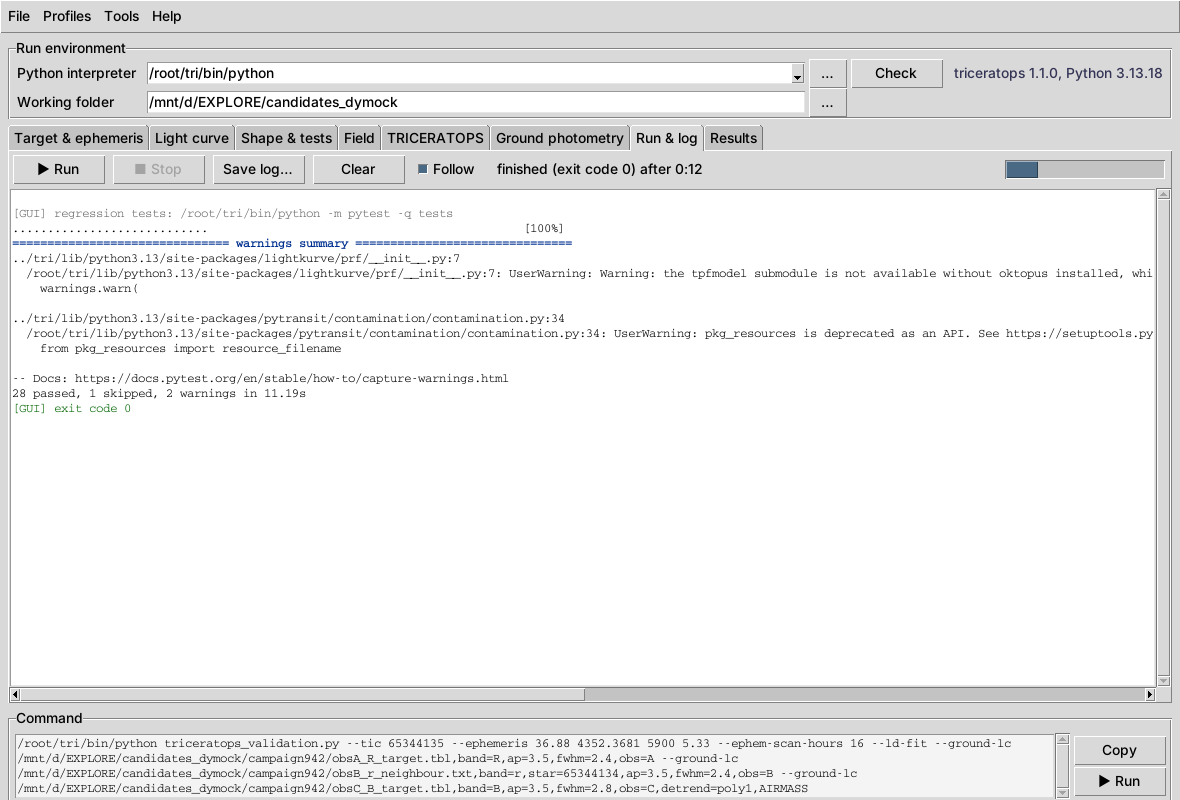
\includegraphics[width=\textwidth]{og_run.png}
\caption{Tab \emph{Run \& log} (here after running the regression tests).}
\label{fig:run}
\end{figure}

\section*{Step 5 --- Read the results}
When the run ends, the tab \emph{Results} opens (Figure~\ref{fig:res}). On
the left is the summary as a tree, on the right the output files; a double
click opens one. The key items:

\begin{longtable}{@{}p{0.27\textwidth}p{0.66\textwidth}@{}}
\toprule
\textbf{Summary item} & \textbf{How to read it}\\
\midrule\endhead
\code{ld_fit} & Radius ratio, impact parameter $b$, \code{grazing}. A grazing fit ($b+k>1$) favours an EB.\\
\code{secondary} & Best secondary eclipse and the 3$\sigma$ depth limit; a detection means EB.\\
\code{etv} & O$-$C scatter, odd/even timing, limits on a third body.\\
\code{ground} $\rightarrow$ \code{target_status} & \emph{consistent}: the target shows the expected dip. \emph{excluded}: it does not, so a likely false positive (check the data first!).\\
\code{ground} $\rightarrow$ \code{cleared} & Neighbours excluded by the ground data and removed before TRICERATOPS.\\
\code{ground} $\rightarrow$ \code{chromaticity} & $p$ of a band-independent depth; \code{chromatic = True} means EB or blend.\\
FPP, NFPP, verdict & See Chapter~2: PASSED when FPP $<0.015$ and NFPP $<0.001$; ``not converged'' means provisional.\\
\code{scenario_classes} & Probability per family: planet on the target, EB on the target/companion, background star, nearby star.\\
\code{triceratops_criteria_met}, \code{eb_evidence}, \code{eb_hints} & Whether FPP and NFPP alone meet the criteria; the pipeline's own evidence that overrules them; notes such as a possible planetary occultation.\\
\code{ld_depth_not_adopted} & Why the depth of the limb-darkened fit was not passed to TRICERATOPS.\\
\code{recommendations} & The next observations (Chapter~\ref{ch:followup}); also in \code{recommendations_<tic>.txt}.\\
\bottomrule
\end{longtable}

\begin{figure}[ht]
\centering
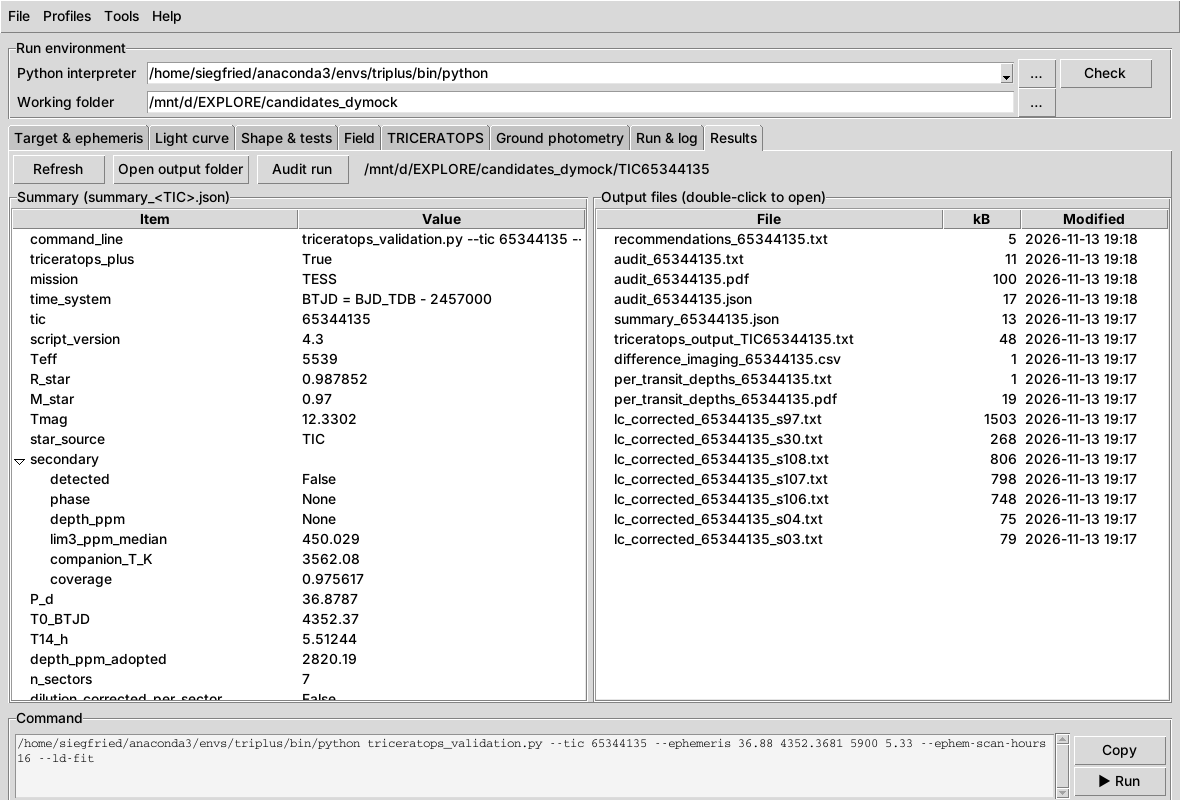
\includegraphics[width=\textwidth]{og_results.png}
\caption{Tab \emph{Results} after the TESS-only run of TIC~65344135 and its
audit: summary (left), output files (right) and the button \emph{Audit run}.}
\label{fig:res}
\end{figure}

\section*{How to interpret the outcomes for TIC 65344135}
\begin{longtable}{@{}p{0.42\textwidth}p{0.51\textwidth}@{}}
\toprule
\textbf{Ground result} & \textbf{Consequence}\\
\midrule\endhead
Target: dip of $\approx$5.9~ppt; neighbour: flat & Neighbour cleared, NFPP $\approx 0$. The FPP is then decided by the shape of the transit and the remaining scenarios on the target.\\
Target flat; neighbour: dip of $\approx$7~ppt & Nearby eclipsing binary: false positive. The log says ``probable nearby eclipsing binary''.\\
Dip on the target but much shallower or deeper than 5.9~ppt & Check the aperture radius, the comparison stars and the time window. If the result is confirmed, the dilution model or the host is wrong.\\
Depth differs between red and blue & Chromatic: EB or blend, even if the dip is on the target.\\
Light curves do not cover the transit & \emph{unconstrained}: no conclusion; a later transit is needed.\\
\bottomrule
\end{longtable}

\textbf{Example from a real run.} For TIC~229788204 (TESS only) the
pipeline found a V-shaped, grazing eclipse with no secondary, an FPP of 1.00,
and probabilities of 0.55 for EB, 0.31 for EBx2P and 0.14 for PEBx2P. This is
the typical signature of an eclipsing binary, here most likely a pair of
nearly equal stars at twice the period (187.7~d).

\section*{Step 6 --- Audit and next observations}
Press \emph{Audit run}. The audit report opens as a PDF; its page \emph{Next
observations} (Figure~\ref{fig:audit-next}) says which observation would
lower the FPP most, and which combination would reach the validation limits.
Chapter~\ref{ch:followup} explains how to read it.

\textbf{Note.} The numbers in Figures~\ref{fig:glc} and~\ref{fig:gclear}
come from a \emph{synthetic} test that mimics the campaign. The first real TESS-only result for this star is in
Chapter~\ref{ch:prelim}.

%% ----------------------------------------------------------------------
\chapter{Preliminary result: TIC 65344135 with TESS only}
\label{ch:prelim}

This chapter reports the first complete run on the real TESS data of
TIC~65344135, made on 4~November 2026 before the campaign transits. It is
the baseline that the ground-based light curves will improve on. The figures
are the pipeline's own output for this star.

\section*{Set-up}
\begin{itemize}
\item \textbf{Command.} Profile \code{profile_TIC65344135} in the
\code{triplus} environment (TRICERATOPS+ 1.0.17, NumPy 2.3, pytransit 2.2):
\begin{lstlisting}
triceratops_validation.py --tic 65344135 --ephemeris 36.88 4352.3681 5900 5.33 --ephem-scan-hours 16 --ld-fit --tri-plus on
\end{lstlisting}
\item \textbf{Data.} TESScut full-frame images of 7 sectors (3, 4, 30, 97,
106, 107, 108; 2018--2026), with cadences of 30, 10 and 3.3~min.
\item \textbf{Dilution.} In every sector the optimal aperture contains the
target and the neighbour TIC~65344134 (5.9$''$). The target supplies a
fraction $g = 0.556$--$0.562$ of the light in the aperture
(Figure~\ref{fig:p-field}).
\item \textbf{TRICERATOPS.} 20 runs, all valid, evidences pooled (re-run of
4~November with the corrected script); no ground-based light curves yet.
\end{itemize}

\begin{figure}[ht]
\centering
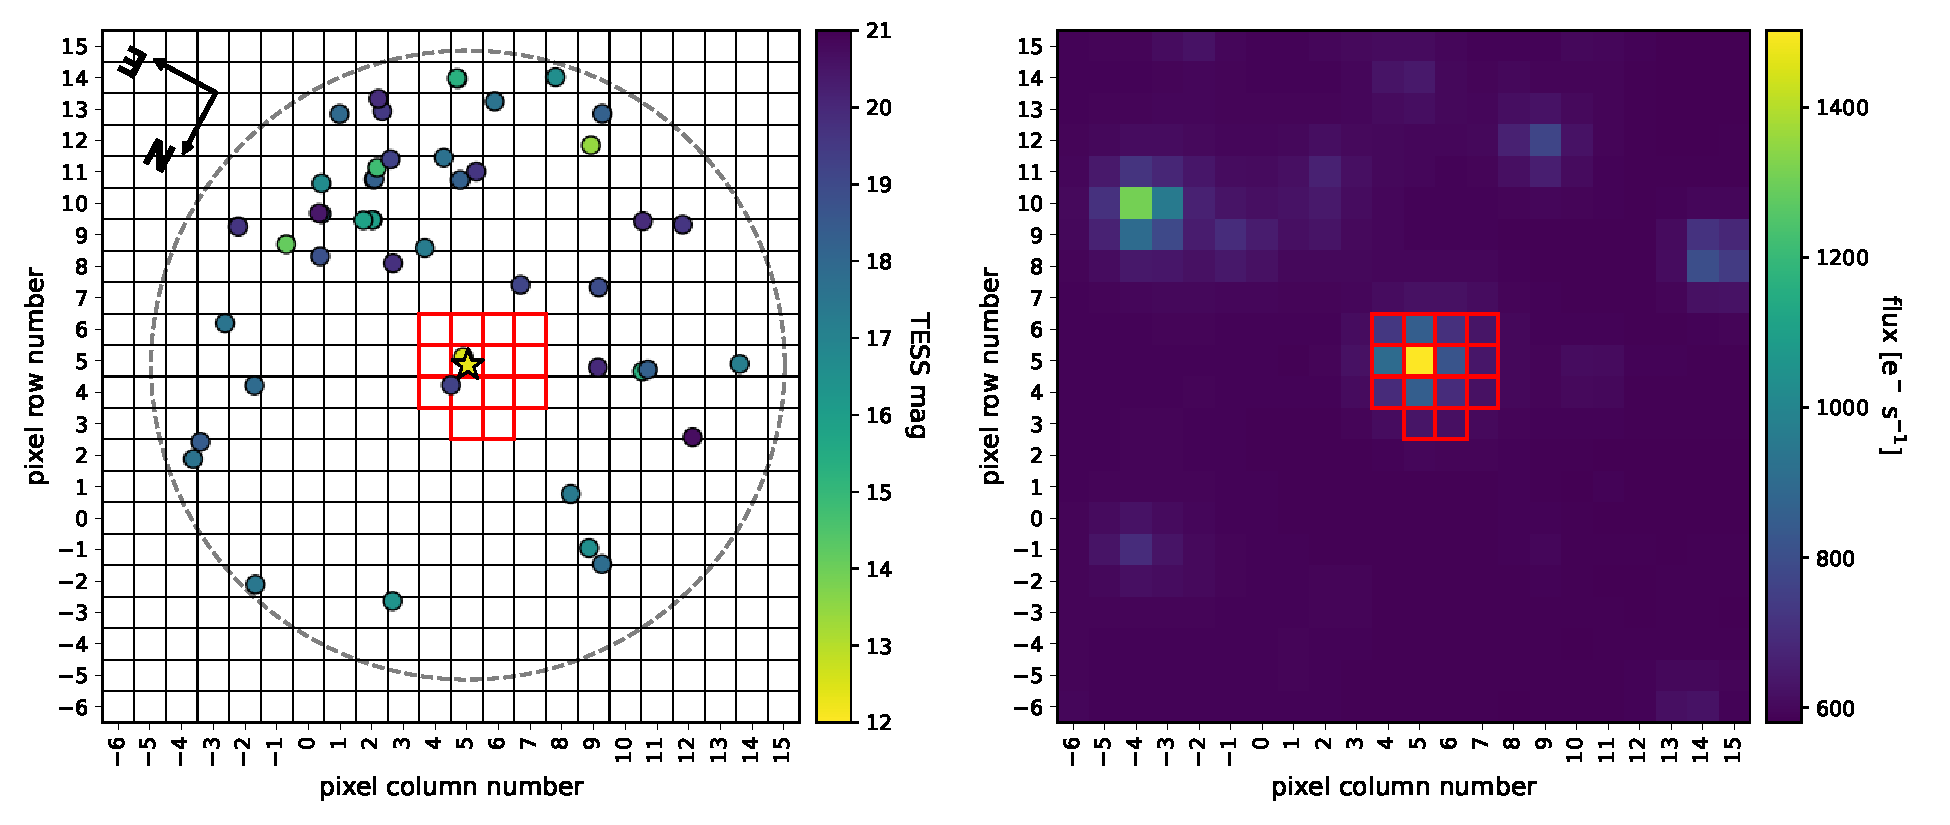
\includegraphics[width=0.95\textwidth]{field_65344135_s97.pdf}
\caption{Sector 97: TIC stars on the TESS pixel grid (left) and the image
with the optimal aperture (red, right). Target and neighbour are 0.28 pixel
apart.}
\label{fig:p-field}
\end{figure}

\section*{Results}

\begin{longtable}{@{}p{0.36\textwidth}p{0.57\textwidth}@{}}
\toprule
\textbf{Quantity} & \textbf{Result}\\
\midrule\endhead
Transits in TESS & 7 (epoch $-2$, sector 107, weak: S/N 2.6).\\
Refined ephemeris & P = 36.87868 $\pm$ 0.00006~d, T0 = BJD 2461352.37156 $\pm$ 0.00225 (3.2~min).\\
Depth in the TESS aperture & 3060~ppm (limb-darkened fit); 2825 $\pm$ 117~ppm (per-transit mean).\\
Depth on the target alone & 5320 $\pm$ 210~ppm if the target is the host (aperture depth / $g$).\\
Duration T14 & 5.49~h.\\
Shape & U-shaped, not grazing; $b \approx 0$ (poorly constrained). $R_p/R_\star = 0.051$ on the aperture scale, 0.068 after the dilution correction ($/\sqrt{g}$). With the TIC radius of 0.99~$R_\odot$ that is about 7.3~$R_\oplus$ if the target is the host (TRICERATOPS, TP scenario: 7.5~$R_\oplus$), a sub-Saturn.\\
Odd/even depths & 0.9$\sigma$ difference: no sign of an EB at twice the period.\\
Secondary eclipse & None; 3$\sigma$ limit 450~ppm. An eclipsing companion would be cooler than about 3560~K.\\
Timing (ETV) & O$-$C rms 9.4~min; no significant period change or third body.\\
Difference imaging & Centroid consistent with the target (median 0.9$\sigma$), but 5.9$''$ cannot be resolved this way.\\
FPP (pooled over 20 runs) & 0.389 $\pm$ 0.014 (run-to-run scatter 0.06).\\
NFPP (pooled over 20 runs) & 0.376 $\pm$ 0.014.\\
Verdict & NOT passed (requires FPP $<$ 0.015 and NFPP $<$ 0.001).\\
\bottomrule
\end{longtable}

\begin{figure}[ht]
\centering
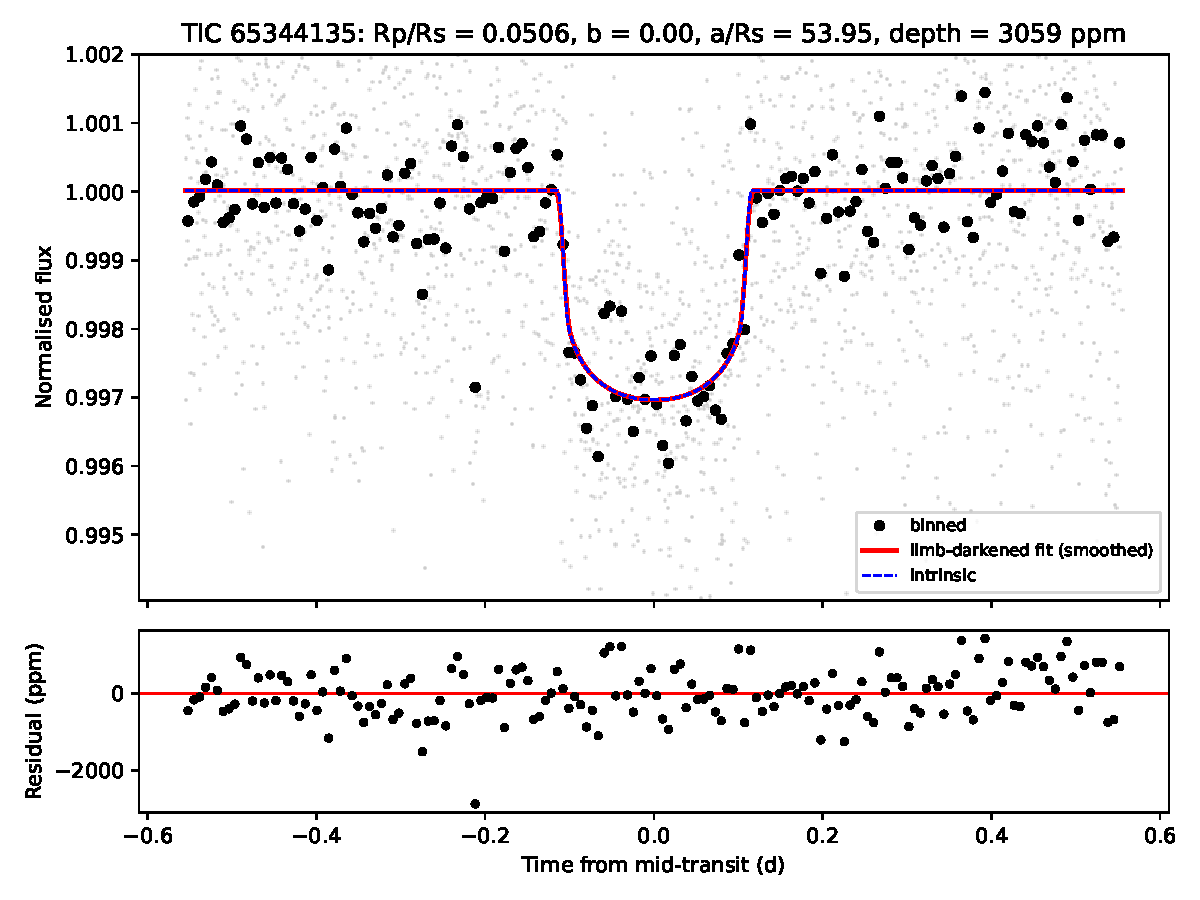
\includegraphics[width=0.62\textwidth]{ld_fit_65344135.pdf}
\caption{Folded TESS light curve of the 7 transits (aperture scale; 10-min
bins) with the limb-darkened fit: a flat-bottomed transit of 3060~ppm and
5.5~h.}
\label{fig:p-ld}
\end{figure}

\begin{figure}[ht]
\centering
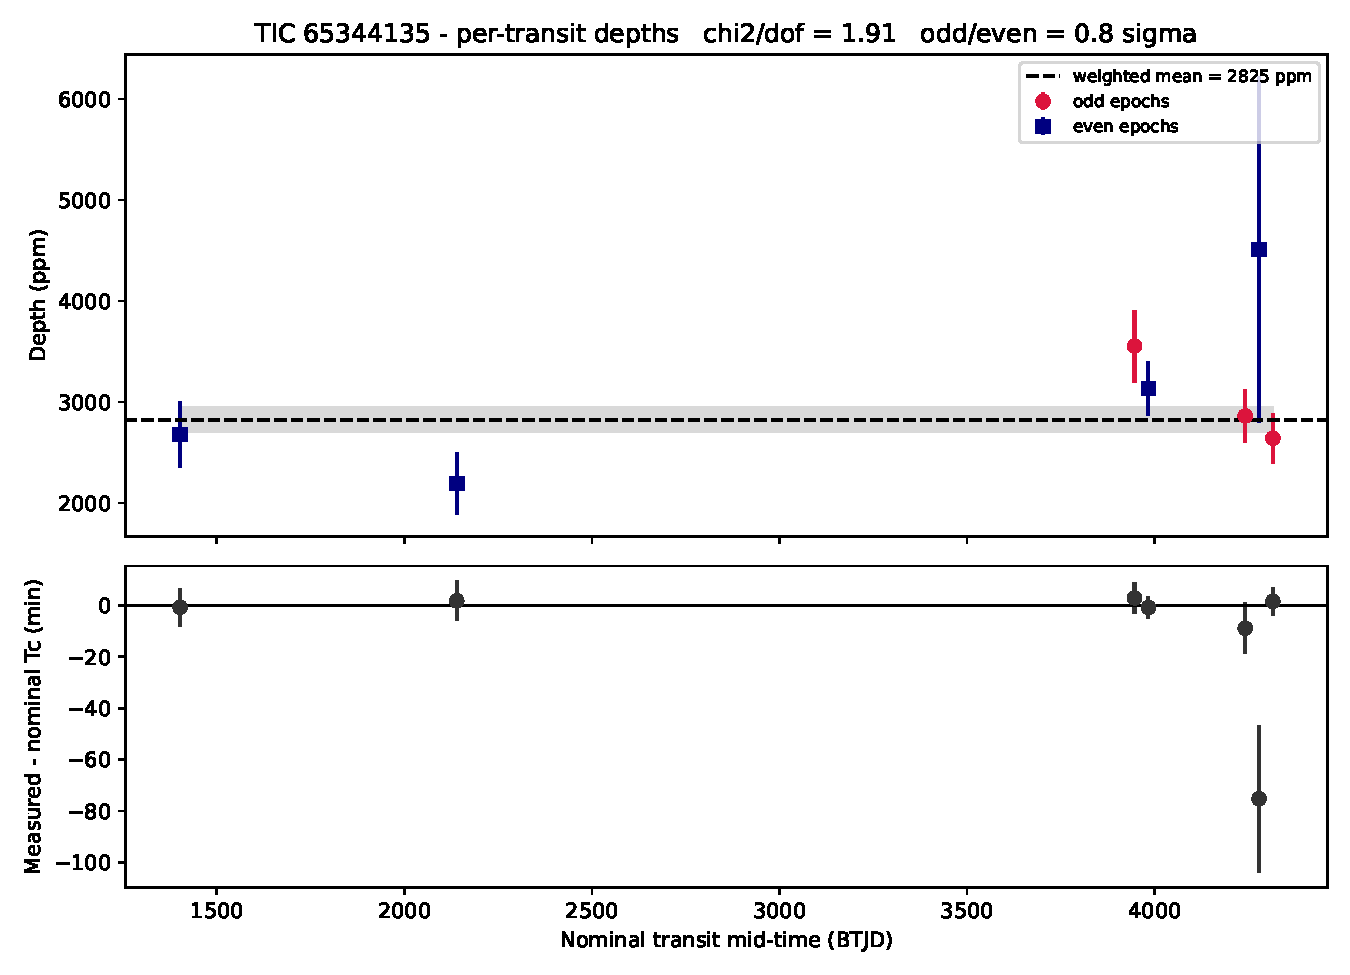
\includegraphics[width=0.62\textwidth]{per_transit_depths_65344135.pdf}
\caption{Depth (top) and mid-time offset (bottom) of the individual
transits. Odd and even transits agree; the outlier at BTJD~4279 is the weak
sector-107 event.}
\label{fig:p-pt}
\end{figure}

\section*{What the probabilities say}

The probability is shared between two explanations
(Figure~\ref{fig:p-classes}):
\begin{itemize}
\item a planet on the target (TP, PTP, DTP): 0.61;
\item a planet on the neighbour TIC~65344134 (NTP): 0.38.
\end{itemize}
The evidences of the TP and NTP scenarios are practically identical
(pooled: 0.43 for TP, 0.38 for NTP). This is expected: the two stars
are almost twins (Tmag 12.33 and 12.56, $T_{\rm eff}$ 5540 and 5390~K), so
the same planet fits on either. Eclipsing-binary scenarios together have
1.4\%, background stars 0.02\%.

\textbf{The light curve itself therefore looks like a planet; what TESS
cannot tell is around which star.} The FPP is high only because of the
neighbour (FPP $\approx$ NFPP).

\begin{figure}[ht]
\centering
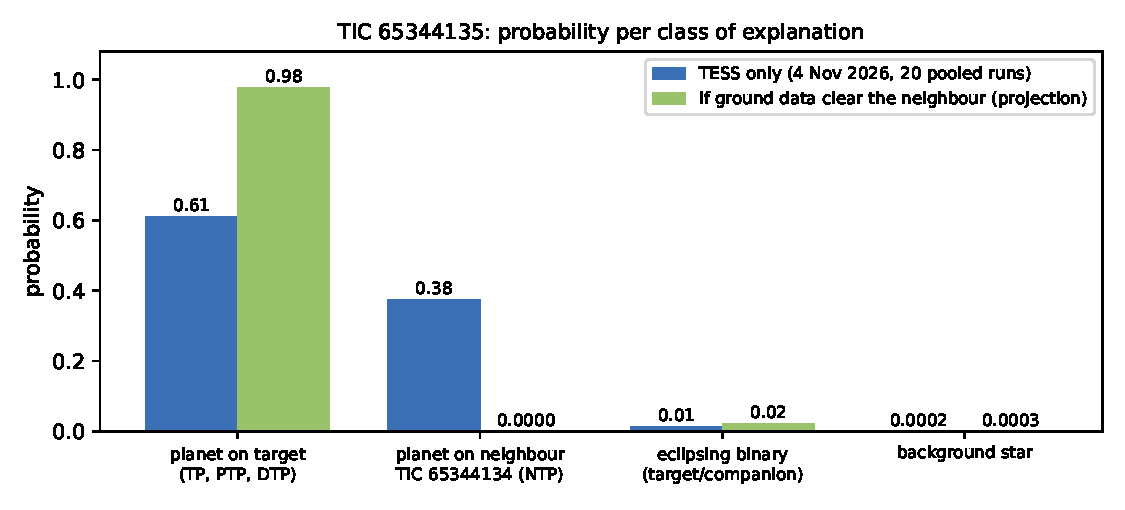
\includegraphics[width=0.85\textwidth]{tic65344135_classes.pdf}
\caption{Probability per class of explanation from the TESS data (blue),
and the projection if the ground photometry clears the neighbour (green).}
\label{fig:p-classes}
\end{figure}

\section*{What the campaign can decide}

\begin{longtable}{@{}p{0.37\textwidth}p{0.56\textwidth}@{}}
\toprule
\textbf{Ground result} & \textbf{Expected effect}\\
\midrule\endhead
Neighbour flat, target dip $\approx$5.3~ppt & TIC 65344134 removed: NFPP $\rightarrow$ 0. FPP $\approx$ 0.014/0.625 $\approx$ 0.02: a \emph{likely planet}, but not yet below 0.015.\\
Target flat, neighbour dip $\approx$6.9~ppt & Nearby eclipsing binary: the candidate is a false positive.\\
Depth differs between red and blue & Chromatic: blend or EB, even on the target.\\
\bottomrule
\end{longtable}

After clearing the neighbour, the remaining 2\% come mostly from
scenarios with an unresolved companion of the target: STP (planet on the
companion) and SEB.

\section*{Recommended next observations (pipeline v4.3)}
The run of 12~November 2026 with v4.3 (TRICERATOPS+, aperture depth, 20
pooled runs) gives the same picture: FPP = 0.391, NFPP = 0.375, a planet on
the target 0.61, a planet on the neighbour 0.37, a companion of the target
(STP, SEB) 0.016. Its page \emph{Next observations}
(Figure~\ref{fig:audit-next}) ranks the follow-up as follows:

\begin{longtable}{@{}p{0.42\textwidth}p{0.14\textwidth}p{0.14\textwidth}p{0.2\textwidth}@{}}
\toprule
\textbf{Observation} & \textbf{FPP best case} & \textbf{FPP typical} & \textbf{NFPP}\\
\midrule\endhead
Now (TESS only) & 0.391 & 0.391 & 0.375\\
Ground photometry, separate apertures & 0.026 & 0.026 & 0\\
\quad + reconnaissance spectroscopy & 0.0004 & 0.008 & 0\\
\quad + transits in g$'$ and z$'$ & 0 & 0.009 & 0\\
\quad + high-resolution imaging & 0 & 0.012 & 0\\
\bottomrule
\end{longtable}

\begin{itemize}
\item \textbf{First the ground transit.} 96\% of the FPP comes from the
neighbour. One transit with a separate aperture on each star decides where
the dip is; with the dip on the target the NFPP drops to zero, and the FPP to
about 0.026.
\item \textbf{Then one of three.} What remains is a planet on an unresolved
companion of the target (STP, best fit 0.71~$M_\odot$, 20\% of the light) or
an eclipsing companion (SEB). Each of the three observations brings the FPP
below 0.015 in its typical outcome. Spectroscopy reaches companions at every
separation; imaging only those wider than 0.1$''$ (37~au), about half of them.
For the colour test, two thirds of the possible companions change the depth
by more than 20\% between g$'$ and z$'$; for the best-fit companion the two
depths would differ by about 1900~ppm, so a depth error of about 600~ppm per
filter is needed.
\item \textbf{A practical choice for the campaign:} observe the transit with
separate apertures \emph{and} in two filters (two telescopes, or alternating
filters). One night then answers both questions.
\end{itemize}

\section*{Updated times for the observers}

The refined ephemeris puts the transits about 5~min later than the campaign
page. UTC times are derived from the campaign page's conversion of BJD to
UTC, with T14 = 5.49~h. Add $\pm$3~min uncertainty plus at least 1~h of
baseline before and after.

\begin{longtable}{@{}lccccc@{}}
\toprule
\textbf{Date} & \textbf{Mid BJD\_TDB} & \textbf{Ingress} & \textbf{Mid} & \textbf{Egress} & \textbf{vs.\ campaign}\\
\midrule\endhead
7 Nov 2026 & 2461352.3716 & 18:03 UTC & 20:48 UTC & 23:33 UTC & +5.0 min\\
14 Dec 2026 & 2461389.2502 & 15:11 UTC & 17:56 UTC & 20:40 UTC & +5.5 min\\
\bottomrule
\end{longtable}

The ground aperture should show these depths:
\begin{itemize}
\item on the target alone, about 5.3~ppt if it is the host;
\item on the neighbour alone, about 6.9~ppt if it is the host;
\item in an aperture holding both stars, about 3.1~ppt.
\end{itemize}

\section*{Remarks}
\begin{itemize}
\item \textbf{Pooled FPP.} In the first run of 4~November the pooled FPP
(0.335, bootstrap error 0.000) was not valid: with TRICERATOPS+ the evidences
of the first run were reused for all 20 runs. The numbers in this chapter come
from the re-run with the corrected script. The pooled evidences are now
consistent with the mean over the runs (0.39), and no single run dominates
(largest share 0.07).
\item \textbf{Stellar density.} The density from the transit shape
(2.2~g\,cm$^{-3}$) is somewhat higher than that from the TIC mass and radius
(1.4~g\,cm$^{-3}$). With $b$ unconstrained and a possible eccentric orbit,
this is no reason for concern.
\end{itemize}

%% ----------------------------------------------------------------------
\chapter{Control target: WASP-18 b}
\label{ch:wasp18}

Before a pipeline is trusted with a new candidate, it should be run on a
planet whose answer is known. WASP-18~b (TIC~100100827) is a good choice: a
hot Jupiter of about 10 Jupiter masses on a 0.94-day orbit around a
$T_\mathrm{mag} = 8.8$ F6 star (Hellier et al.\ 2009), observed by TESS in
ten sectors between 2018 and 2026. The transit is 1~\% deep, and the planet
is so hot that TESS also sees it disappear behind the star: an
\emph{occultation} (secondary eclipse) of about 340~ppm at phase 0.5
(Shporer et al.\ 2019). A pipeline that validates WASP-18~b, finds its
occultation and does \emph{not} mistake that occultation for the sign of an
eclipsing binary, passes an honest test. This chapter shows that run and
what it taught us.

\section*{Set-up}
The profile \code{profile_WASP18b.json} (menu \emph{Profiles}) contains:
\begin{lstlisting}
"tic": "100100827", "outdir": "WASP18b",
"blind_search": true, "p_min": "0.5", "p_max": "10",
"ld_fit": true, "vet_neighbours": true, "sensitivity": true,
"red_noise_scrambles": "2000"
\end{lstlisting}
No period is given: the pipeline must find the planet itself with a blind
TLS search between 0.5 and 10~days. The run uses TESScut full-frame images
of sectors 2, 3, 29, 30, 69, 96, 103, 104, 105 and 106 (cadences 30, 10 and
3.3~min); the optimal apertures of 20--24 pixels contain 99.2--99.6~\% of the
target's light (Figure~\ref{fig:w18-field}). A complete run takes about two
hours, most of it in TRICERATOPS and the red-noise scrambles; the audit is
run afterwards with the button \emph{Audit}.

\begin{figure}[ht]
\centering
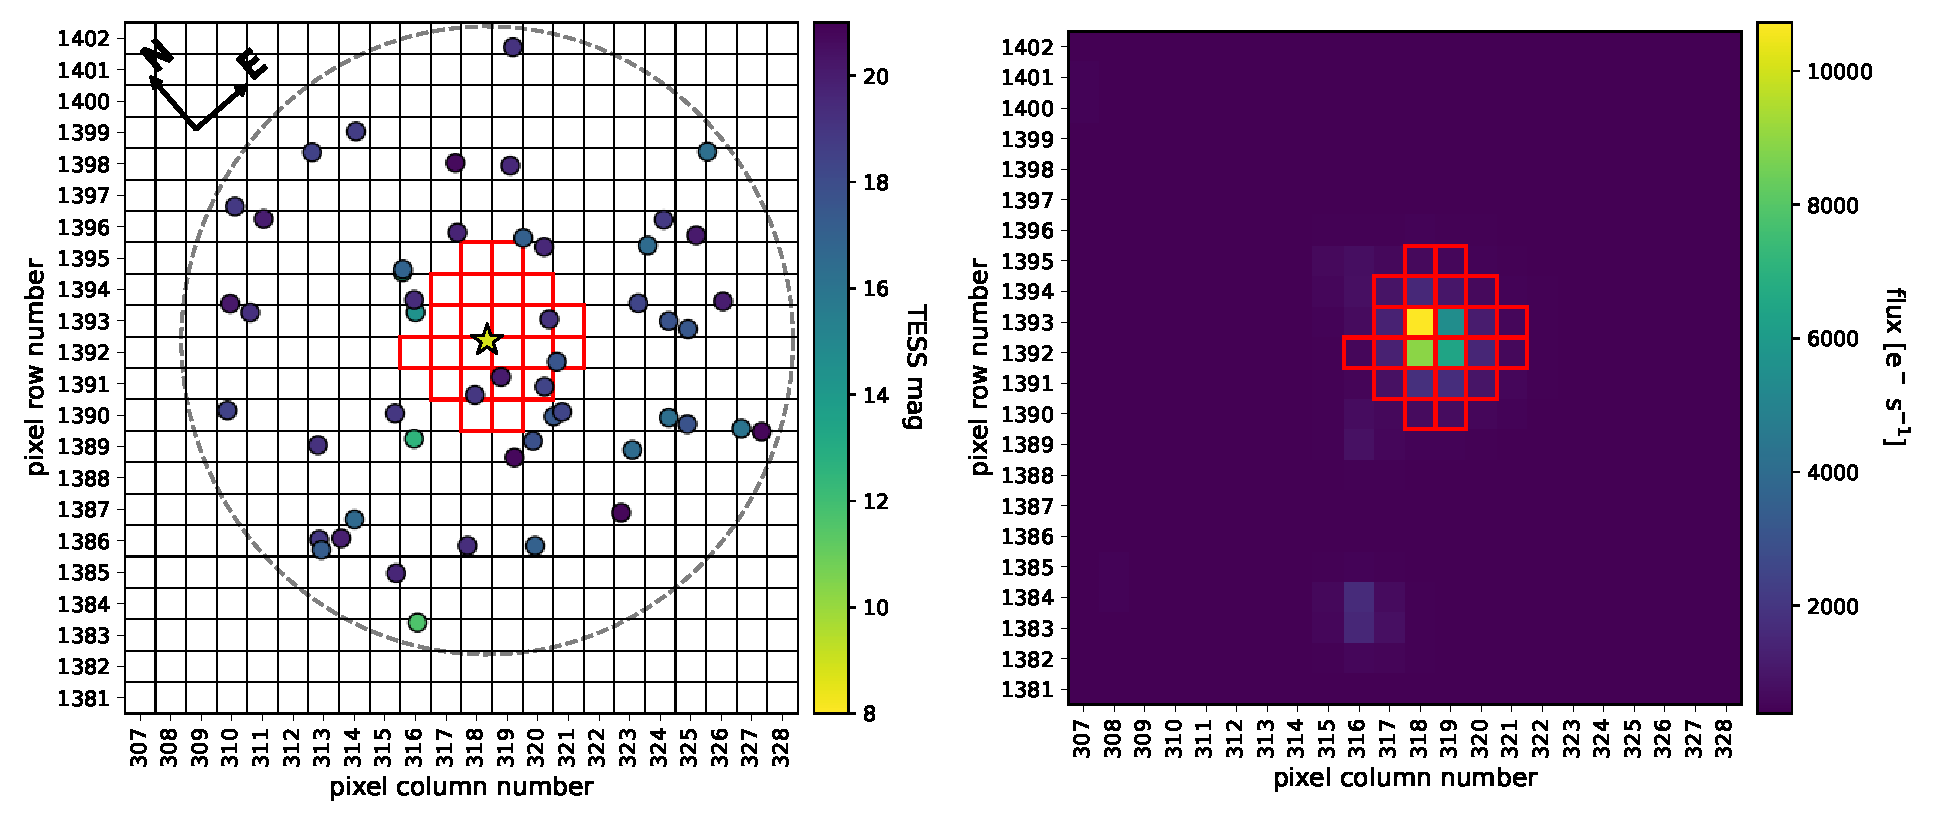
\includegraphics[width=0.85\textwidth]{wasp18_field_s104.pdf}
\caption{Sector 104: TIC stars on the TESS pixel grid (left) and the image
with the optimal aperture (right). WASP-18 is by far the brightest star in
the aperture.}
\label{fig:w18-field}
\end{figure}

\section*{Results}

\begin{longtable}{@{}p{0.33\textwidth}p{0.29\textwidth}p{0.30\textwidth}@{}}
\toprule
\textbf{Quantity} & \textbf{Pipeline} & \textbf{Literature}\\
\midrule\endhead
Period (blind search) & 0.941452~d (ETV fit) & 0.941452~d\\
Transits used & 257 in 10 sectors & ---\\
Duration T14 & 2.19~h & 2.2~h\\
Depth (limb-darkened fit) & 10\,938~ppm & ---\\
Depth (per-transit mean, adopted) & 10\,381 $\pm$ 9~ppm, $\chi^2_\nu = 1.4$ & ---\\
$R_p/R_\star$ & 0.0967 & 0.097\\
Impact parameter $b$ & 0.00 (at the fit limit) & $\approx$0.36\\
Stellar density from the transit & 1.05~g\,cm$^{-3}$ at $b = 0$ & ---\\
Planet radius (TP scenario) & 14.3~$R_\oplus$ = 1.28~$R_\mathrm{J}$ & $\approx$1.2~$R_\mathrm{J}$\\
Odd/even depths & 1.1$\sigma$ & ---\\
Secondary eclipse & phase 0.4985, 387~ppm, S/N 64 & phase 0.5, 341~ppm\\
Brightness temperature & $\approx$2900~K & dayside $\approx$3000~K\\
Timing (ETV) & O$-$C rms 0.7~min; no trend & ---\\
Difference imaging & on the target, median 0.1$\sigma$ (10 sectors) & ---\\
FPP / NFPP & 0 / 0 & ---\\
Verdict & PASSED & confirmed planet\\
\bottomrule
\end{longtable}

\begin{figure}[ht]
\centering
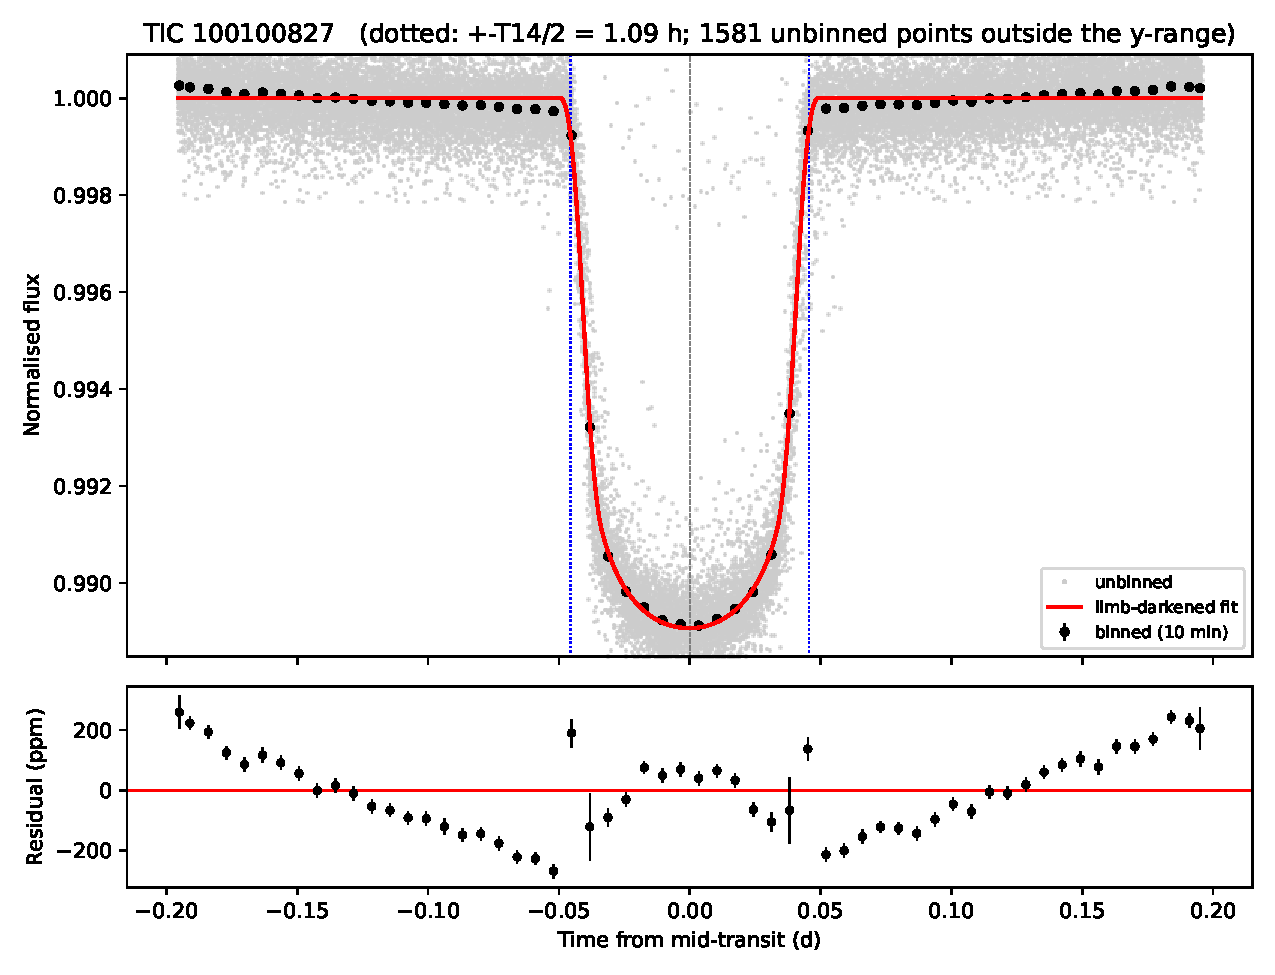
\includegraphics[width=0.49\textwidth]{wasp18_phased_transit.pdf}\hfill
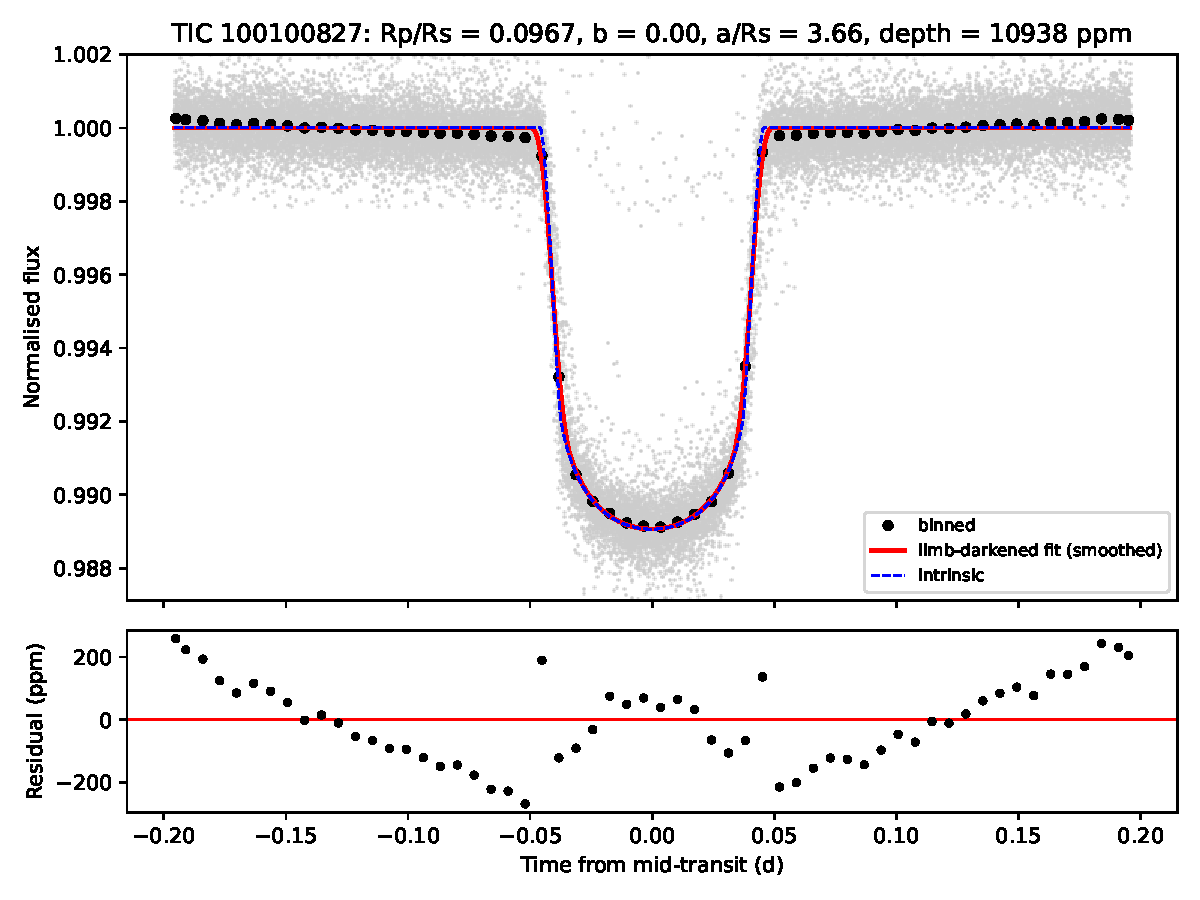
\includegraphics[width=0.49\textwidth]{wasp18_ld_fit.pdf}
\caption{Left: the 254 transits folded on the pipeline ephemeris, with the
limb-darkened fit and 10-min bins. Right: the limb-darkened fit on the
binned fold (smoothed with each sector's cadence). The residuals (lower
panels) are not flat: they show a wave of $\pm$250~ppm. That is not a
problem of the fit but a property of the star: the massive planet raises
tides on it, and its brightness changes twice per orbit (ellipsoidal
variation), on top of the planet's own phase curve.}
\label{fig:w18-transit}
\end{figure}

Two entries in the table deserve a comment.

\textbf{Impact parameter and density.} The fit puts $b$ at its lower limit
0, where the density of the star from the transit shape is
1.05~g\,cm$^{-3}$, against 0.69~g\,cm$^{-3}$ from the TIC mass and radius.
For a hot Jupiter with $R_p/R_\star \approx 0.1$ a central and a slightly
off-centre transit look almost the same in TESS data; the audit therefore
reports that ``$b$ is unconstrained and $b = 0.54$ gives the catalogue
density'', and the pipeline keeps its per-transit depth rather than the
limb-darkened one. The literature value $b \approx 0.36$ lies in between.
This is the normal situation for a deep, short transit; it is not a warning.

\textbf{Depth.} The depth passed to TRICERATOPS is the weighted mean of the
257 individual transits, 10\,381~ppm in the aperture; the limb-darkened fit
gives 10\,938~ppm at the bottom of the transit. Both describe the same
transit: the first is the mean over the box of the transit, the second its
deepest point.

\textbf{The noise used by TRICERATOPS.} The scatter of the binned fold
around the transit model is 160~ppm, while white noise alone would give
24~ppm. The difference is the ellipsoidal wave of
Figure~\ref{fig:w18-transit}. The pipeline uses the measured 160~ppm, which
is conservative: TRICERATOPS is told that the light curve is noisier than
its photon noise. This is why the sensitivity test (below) loses the pass
only when the noise is multiplied by four.

\begin{figure}[ht]
\centering
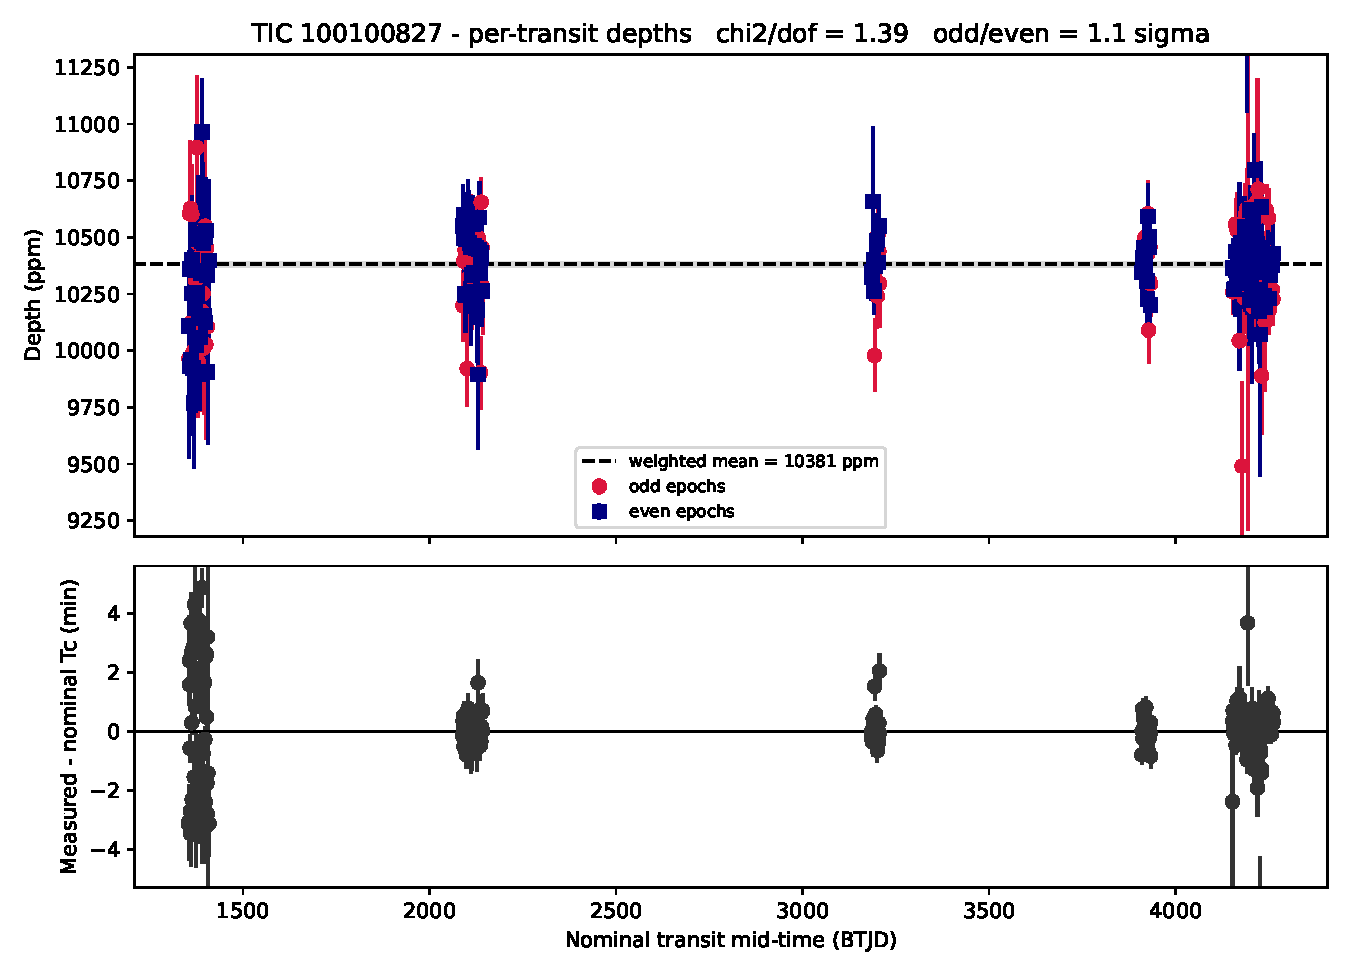
\includegraphics[width=0.62\textwidth]{wasp18_per_transit.pdf}
\caption{Depth (top) and mid-time offset (bottom) of the 257 individual
transits, measured with the trapezoid template. Odd (red) and even (blue)
transits agree (1.1$\sigma$); the depths scatter only 1.4 times their
errors over eight years; the mid-times agree with the linear ephemeris
within 1.3~min rms. The 30-min cadence of 2018 (left) gives the largest
scatter.}
\label{fig:w18-pt}
\end{figure}

\begin{figure}[ht]
\centering
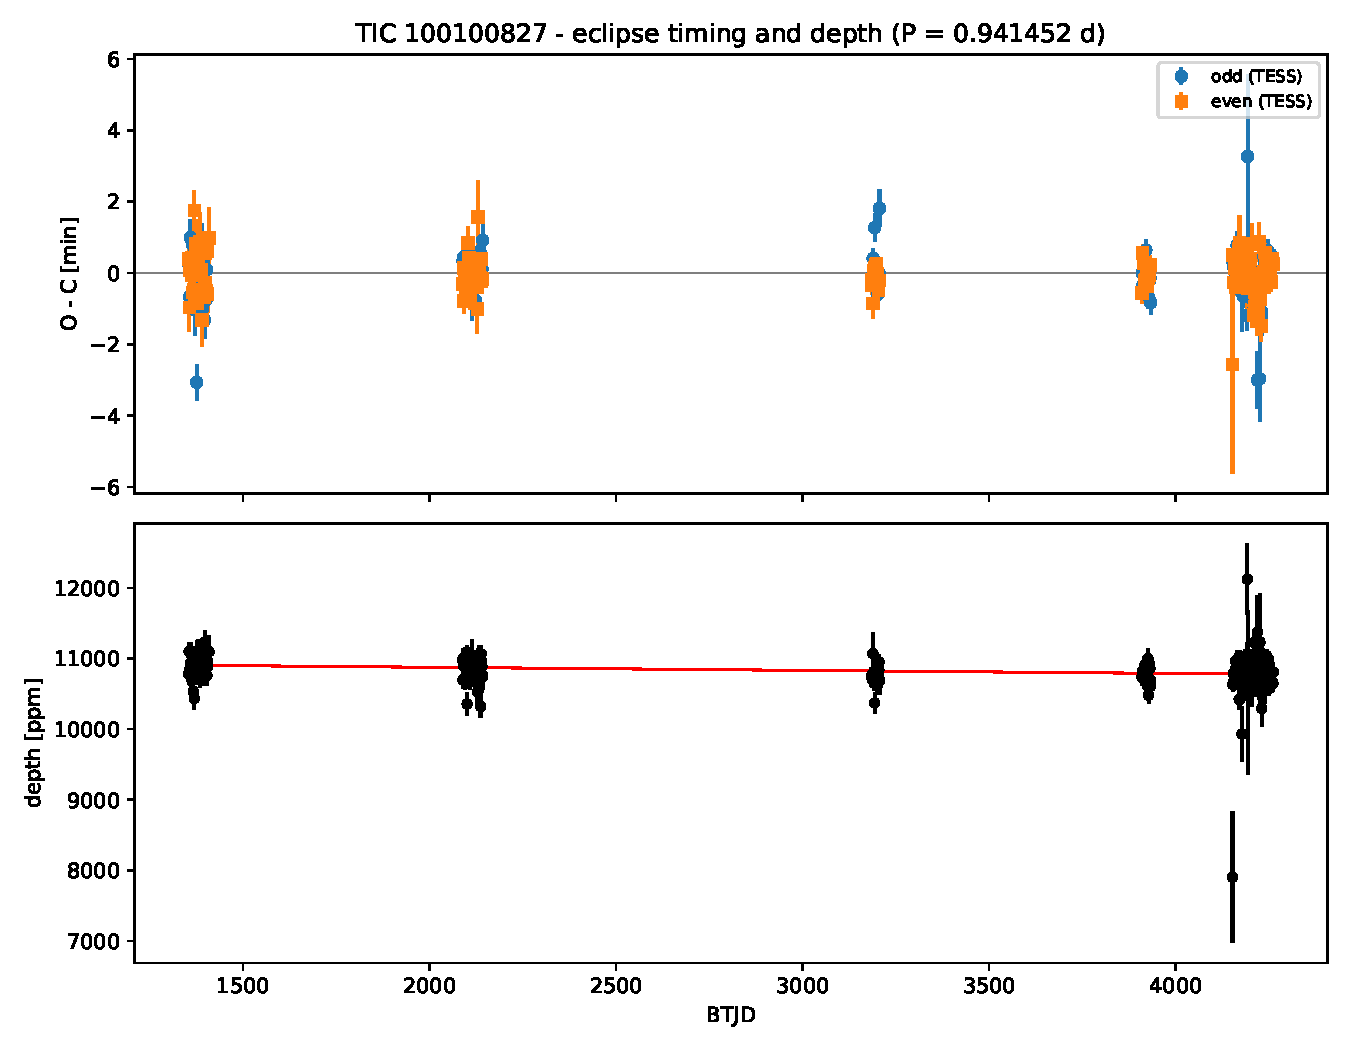
\includegraphics[width=0.62\textwidth]{wasp18_etv.pdf}
\caption{Eclipse timing (top) and depth (bottom) of 256 transits over eight
years. The mid-times scatter by 0.7~min around a constant period; there is
no sign of orbital decay or of a third body within the limits of TESS.}
\label{fig:w18-etv}
\end{figure}

\section*{The secondary eclipse}

The pipeline searches the whole orbit, not only phase 0.5, for a second dip
(Figure~\ref{fig:w18-sec}). For WASP-18 it finds one at phase 0.4985
(less than a minute from 0.5: a circular orbit), 387~ppm deep, with S/N 64
from 244 orbits. The depth ratio secondary/primary gives the surface
brightness of the second body in the TESS band, and from that a brightness
temperature of about 2900~K.

\begin{figure}[ht]
\centering
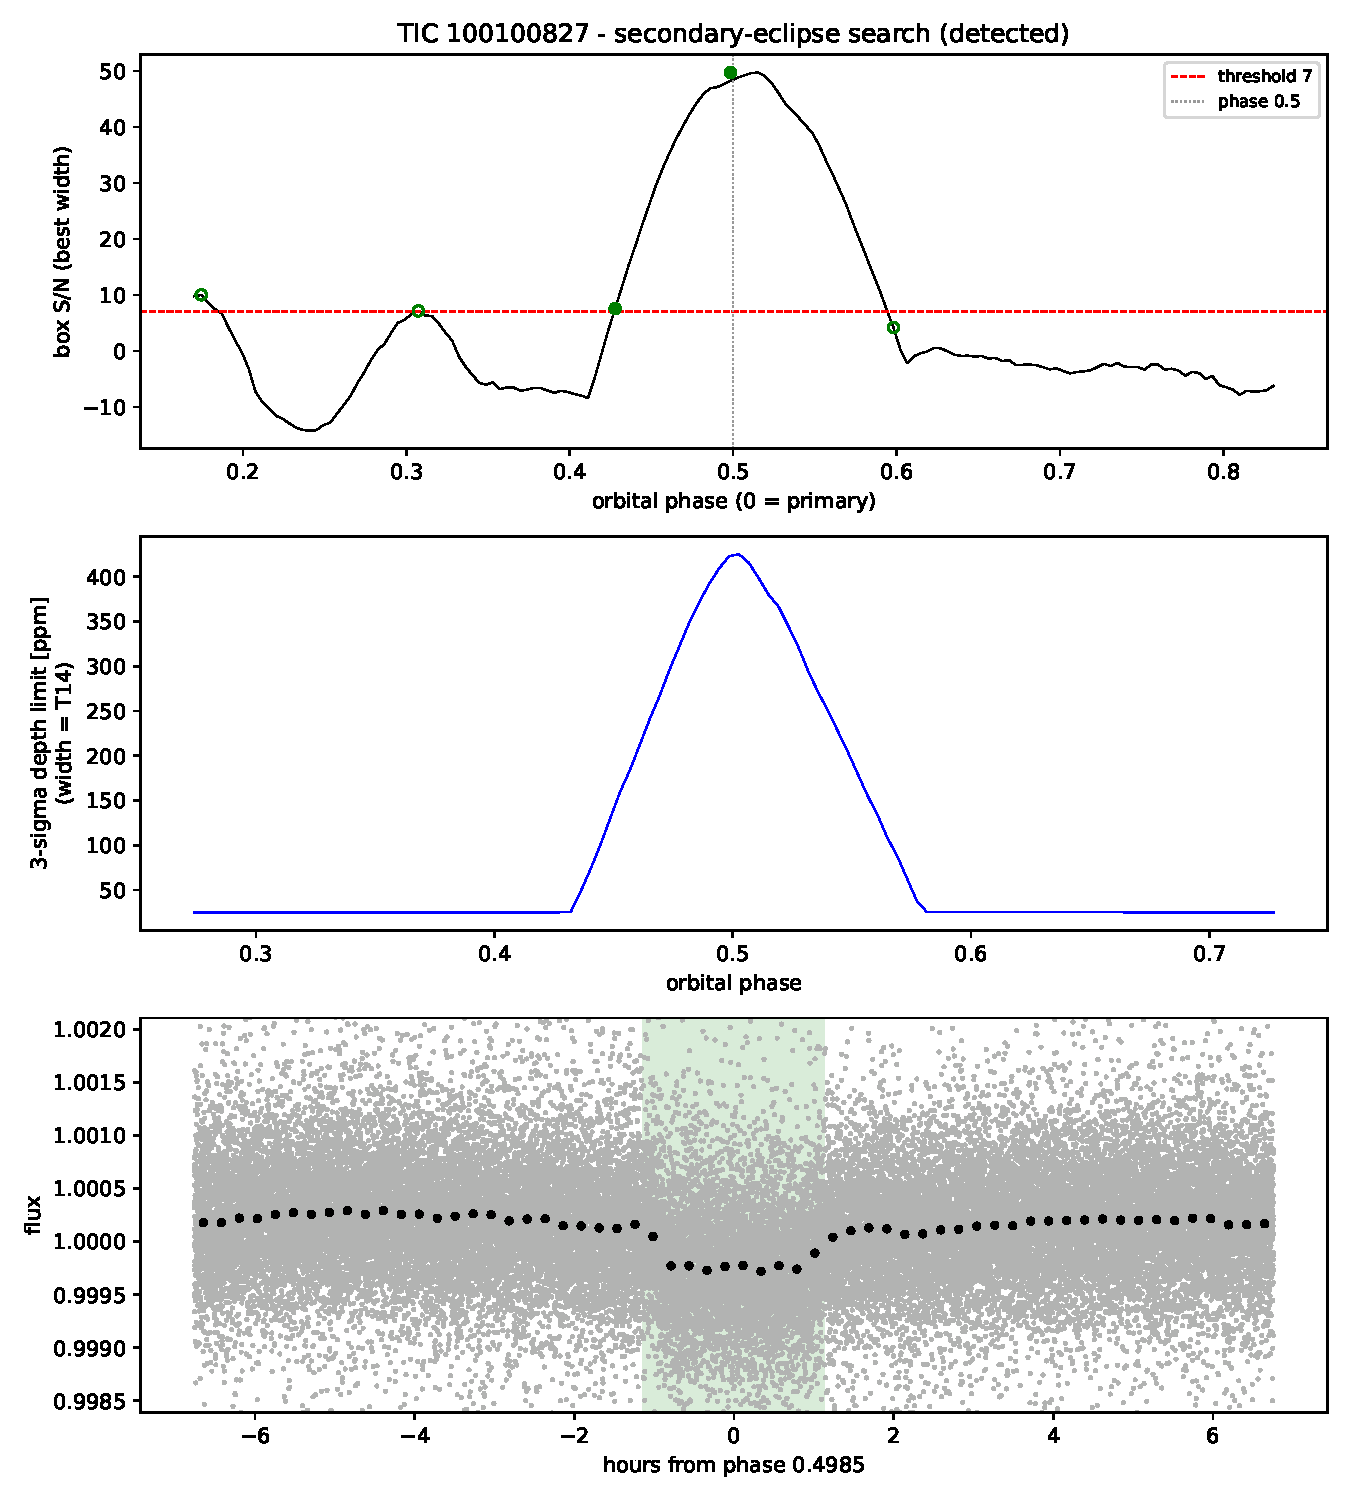
\includegraphics[width=0.7\textwidth]{wasp18_secondary_search.pdf}
\caption{Secondary-eclipse search. Top: S/N of a box search over the
orbital phase; the peak at 0.5 is the occultation. Middle: 3$\sigma$ depth
limit (near the primary no search is possible). Bottom: the light curve
folded on the secondary, with the eclipse window in green.}
\label{fig:w18-sec}
\end{figure}

A secondary eclipse is usually the strongest sign of an eclipsing binary.
Here it must not be: a planet at 2900~K also has a secondary eclipse.
The pipeline therefore applies a simple rule. A secondary eclipse that is
cooler than 4000~K \emph{and} less than 10~\% of the primary depth can be
the occultation of a hot planet; it is reported as a hint
(\code{eb_hints} in the summary) and is not used against the planet. A
self-luminous M dwarf of the same size would show the same signal, so the
audit lists it as a warning and states what decides: a radial-velocity
mass. For WASP-18~b that mass is known (10~$M_\mathrm{J}$): the warning is
correct, and the answer is ``planet''.

The measured 387~ppm is somewhat deeper than the published 341~ppm. The
pipeline measures the eclipse against a local baseline on both sides, and
on this star that baseline is bent by the phase curve; a full phase-curve
model, as in the literature, is beyond the purpose of a validation run.

\section*{Where the signal comes from}

With 99~\% of the light from WASP-18 and a 1~\% transit, the difference
image (out-of-transit minus in-transit) is bright and sharp in every sector
(S/N 1200--2650). Its centroid lies on the target to within 0.03~pixel; the
median offset over the ten sectors is 0.1$\sigma$
(Figure~\ref{fig:w18-di}). All 51 neighbours in the field are excluded as
the source.

\begin{figure}[ht]
\centering
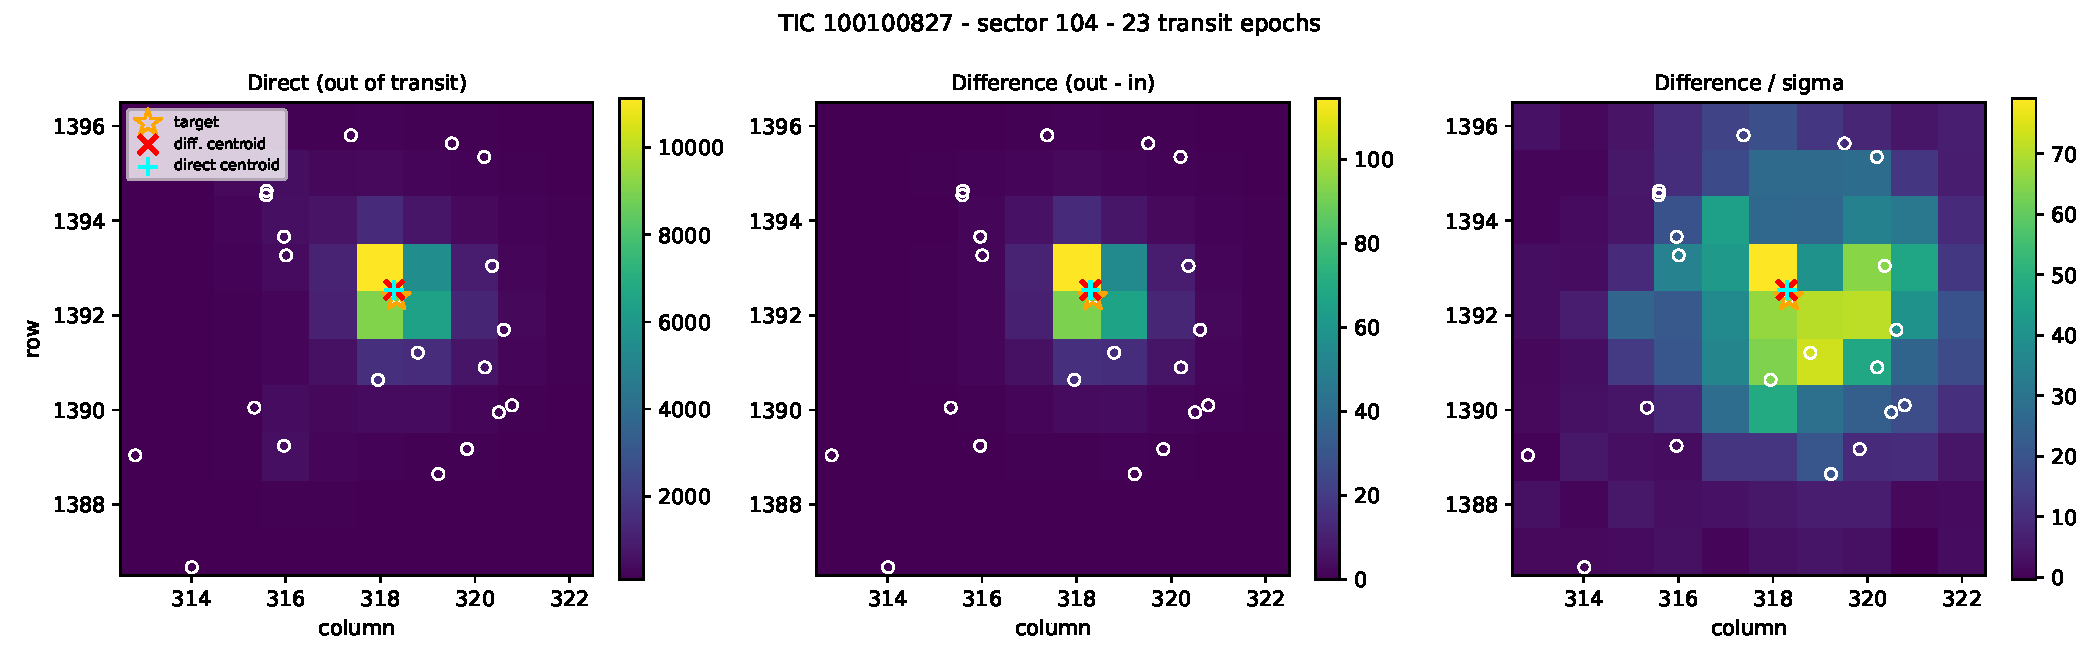
\includegraphics[width=\textwidth]{wasp18_diffimg_s104.pdf}
\caption{Difference imaging, sector 104: direct image (left), difference
image (middle) and difference divided by its error (right). Target, centroid
of the difference image and centroid of the direct image coincide.}
\label{fig:w18-di}
\end{figure}

\section*{TRICERATOPS, audit and next observations}

All 20 TRICERATOPS runs are valid. The probability goes entirely to the
planet scenarios: TP 0.87, PTP 0.07 (planet on the target, with an unseen
bound companion diluting it) and DTP 0.05 (the same with an unresolved
background star). Every other scenario has a probability below
$10^{-17}$: a 1~\% eclipse on a bright star, with a shape this well
measured, leaves no room for them. FPP and NFPP are both 0.

The sensitivity test repeats the calculation with the noise multiplied by
0.5, 2 and 4. The pass holds up to twice the measured noise
(FPP~0.004) and is lost only at four times (FPP~0.029); the audit records
this as a PASS, with the advice to report the table. The audit summary is:
\emph{no FAIL, 1 WARN} (the occultation), 12 PASS, 3 not applicable (no
input ephemeris, no ground data). The page \emph{Next observations} finds
nothing left to remove; for a new candidate of this kind it would point to
a radial-velocity measurement, the only observation that tells a hot
Jupiter from a low-mass star.

\begin{tip}
\textbf{Lessons from the control target.} WASP-18~b exposed four problems
in earlier versions of the pipeline, all fixed in v4.3:
(1)~the blind search used the 5$\times$ wider masking window to refine the
ephemeris: T0 was 4~h off, T14 came out as 9~h and the depth as 100~ppm,
and the fold showed a flat line --- \emph{if T14 or the depth of a known
planet look wrong, suspect the ephemeris first};
(2)~the audit counted every secondary eclipse as a failure, also the
occultation of a hot planet;
(3)~the phase curve pulled the secondary eclipse to phase 0.52;
(4)~in sectors with strong scattered light the difference image had
S/N~$<1$ until bad frames were removed;
(5)~the template for the individual transits came from the TLS search on
binned data and was misaligned: the mid-times were biased by 10--17~min
and the adopted depth by $-9$ to $+9$~\%. The template is now the
trapezoid fitted to the fold on the adopted ephemeris
(Figure~\ref{fig:w18-pt}: mid-times within 1.3~min rms).
Run WASP-18~b again after every change to the pipeline: it takes two
hours, and the answer is known.
\end{tip}


%% ----------------------------------------------------------------------
\chapter{A false positive: the two candidates of TIC 229701403}
\label{ch:tic2297}

The opposite of a control target is a candidate that turns out not to be a
planet. TIC~229701403 ($T_\mathrm{mag} = 10.97$, a G star of
1.16~$R_\odot$, 258~pc) was found by Roger Dymock in TESS data with two long
period candidates of Saturn size:

\begin{center}
\begin{tabular}{@{}lccccc@{}}
\toprule
 & P (d) & T0 (BTJD) & depth (ppm) & T14 (h) & profile\\
\midrule
b & 490.259 & 1951.170 & 7341 & 10.5 & \code{profile_TIC229701403_b}\\
c & 829.124 & 1857.428 & 5470 & 10.2 & \code{profile_TIC229701403_c}\\
\bottomrule
\end{tabular}
\end{center}

Each profile gives the ephemeris of its own candidate and masks the
transits of the other one (\code{--mask-ephemeris}). The star lies near the
northern ecliptic pole and was observed in 40 sectors between 2019 and 2024;
two of them (59 and 86) are excluded automatically for scattered light.
This chapter shows how the pipeline and the audit flag the candidates, and
how a look at \emph{all} the dips together turns two planets into one
eclipsing binary.

\section*{What the runs say}

Both runs end with \emph{NOT passed}, and the audits list four FAIL each:

\begin{itemize}
\item \textbf{Depth consistency.} The three transits of b have on-target
depths of 8090, 12\,480 and 7290~ppm ($\chi^2_\nu = 281$); those of c 4990
and 4440~ppm, and the third predicted transit of c, in sector 81, is
\emph{absent} ($-460 \pm 150$~ppm).
\item \textbf{Odd/even.} 10$\sigma$ (b) and 15$\sigma$ (c).
\item \textbf{Secondary eclipse.} For b the search finds a second dip at
phase 0.308, 1490~ppm deep: far from 0.5, and deep and warm
(3900~K) --- not the occultation of a planet.
\item \textbf{Centroids.} In every sector with a transit the centroid of the
difference image lies 65$''$ (3 pixels) from the target, at
30$\sigma$, on the neighbour TIC~229701402 ($T_\mathrm{mag} = 11.46$,
5300~K; Figure~\ref{fig:t2297-di}).
\end{itemize}

TRICERATOPS gives FPP~$\approx 1$ for b (mostly SEBx2P) and FPP~0.09 for c.
Neither number is the point: the tests above already say that the
candidates are not what they seem.

\begin{figure}[ht]
\centering
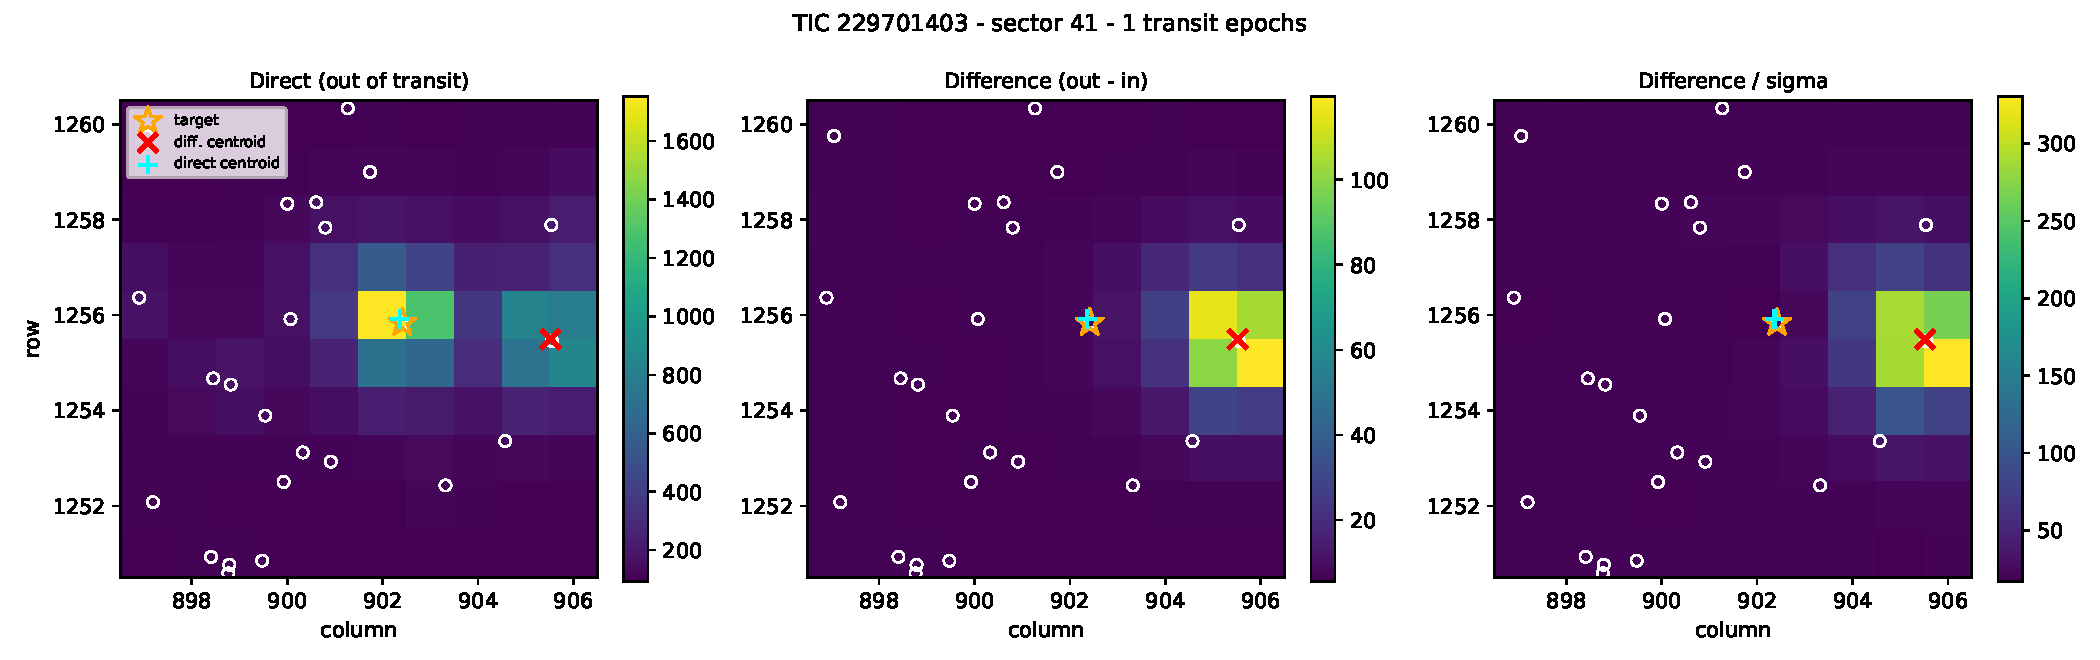
\includegraphics[width=\textwidth]{tic229701403_diffimg_s41.pdf}\\[0.5em]
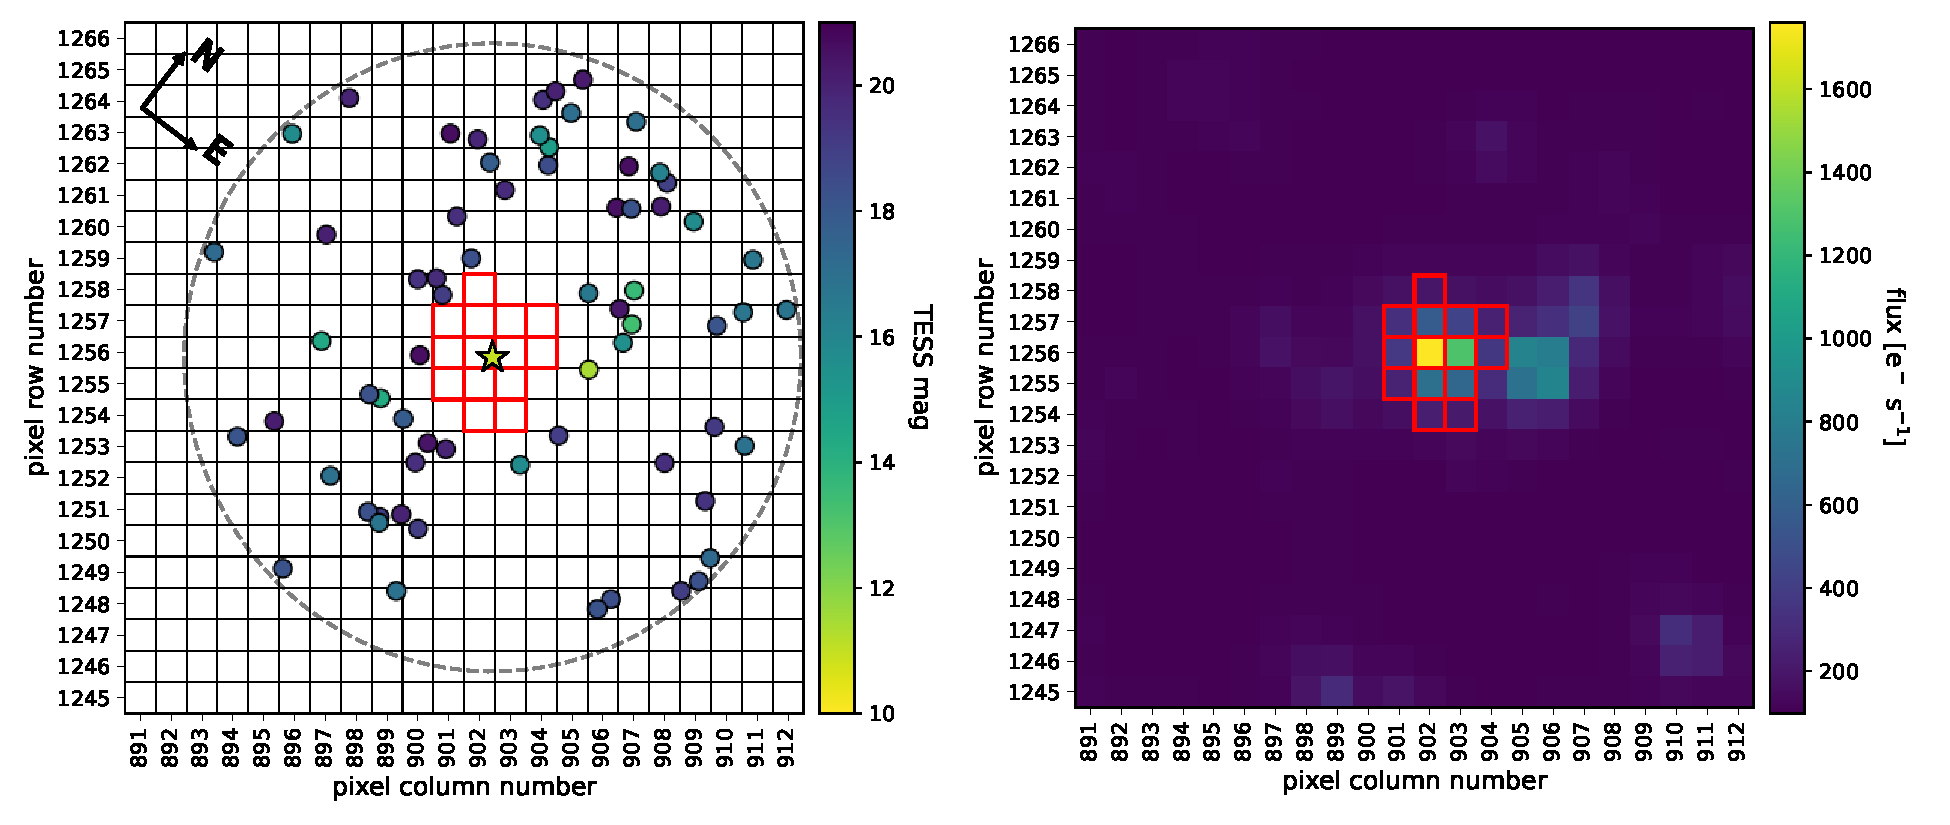
\includegraphics[width=0.75\textwidth]{tic229701403_field_s41.pdf}
\caption{Sector 41, the deepest event (BTJD 2441.43). Top: direct image,
difference image (out of transit minus in transit) and difference over its
error. The target (star symbol) is bright in the direct image, but the
light that disappears comes from the star three pixels to the right, TIC
229701402 (red cross: centroid of the difference image). Bottom: the field
with the optimal aperture (red); the neighbour lies at its edge.}
\label{fig:t2297-di}
\end{figure}

\section*{One period for all dips}

A list of all dips deeper than about 1000~ppm in the 38 good sectors shows
ten clear events. Their times fit a single period of
\textbf{245.13~days}, with the events at two fixed phases
(Figures~\ref{fig:t2297-ecl} and \ref{fig:t2297-time}):

\begin{center}
\begin{tabular}{@{}lll@{}}
\toprule
 & Times (BTJD) & In the aperture\\
\midrule
Primary eclipse, phase 0 & 1706.05, 1951.16, 2441.43, 2686.56, 3421.94 & 3300--9700 ppm\\
Secondary eclipse, phase 0.617 & 1857.39, 2592.76, 2837.93, 3328.20, 3573.29 & 2100--4100 ppm\\
\bottomrule
\end{tabular}
\end{center}

\begin{itemize}
\item The linear fits give $P = 245.1283$~d (primaries, rms 9~min) and
$245.1317$~d (secondaries): the same period.
\item Every predicted eclipse that falls in TESS data is observed; none is
missing. At half the period (122.6~d) no dips are seen, so 245.13~d is the
true period.
\item Candidate \textbf{b} (490.26~d $= 2\times245.13$) used only every
other primary eclipse; the primary at 2686.56 lay between them.
\item Candidate \textbf{c} (829.12~d) joined a secondary eclipse (1857.39)
to a primary (2686.56). Its third ``transit'' was therefore predicted at a
time when nothing happens: the absent event in sector 81.
\item The ``secondary eclipse at phase 0.308'' of the b run is the real
secondary eclipse, seen on the double period:
$0.617/2 = 0.308$.
\item A secondary eclipse at phase 0.617 instead of 0.5 means an eccentric
orbit: $e\cos\omega \approx \tfrac{\pi}{2}(0.617-0.5) = 0.18$.
\end{itemize}

\begin{figure}[ht]
\centering
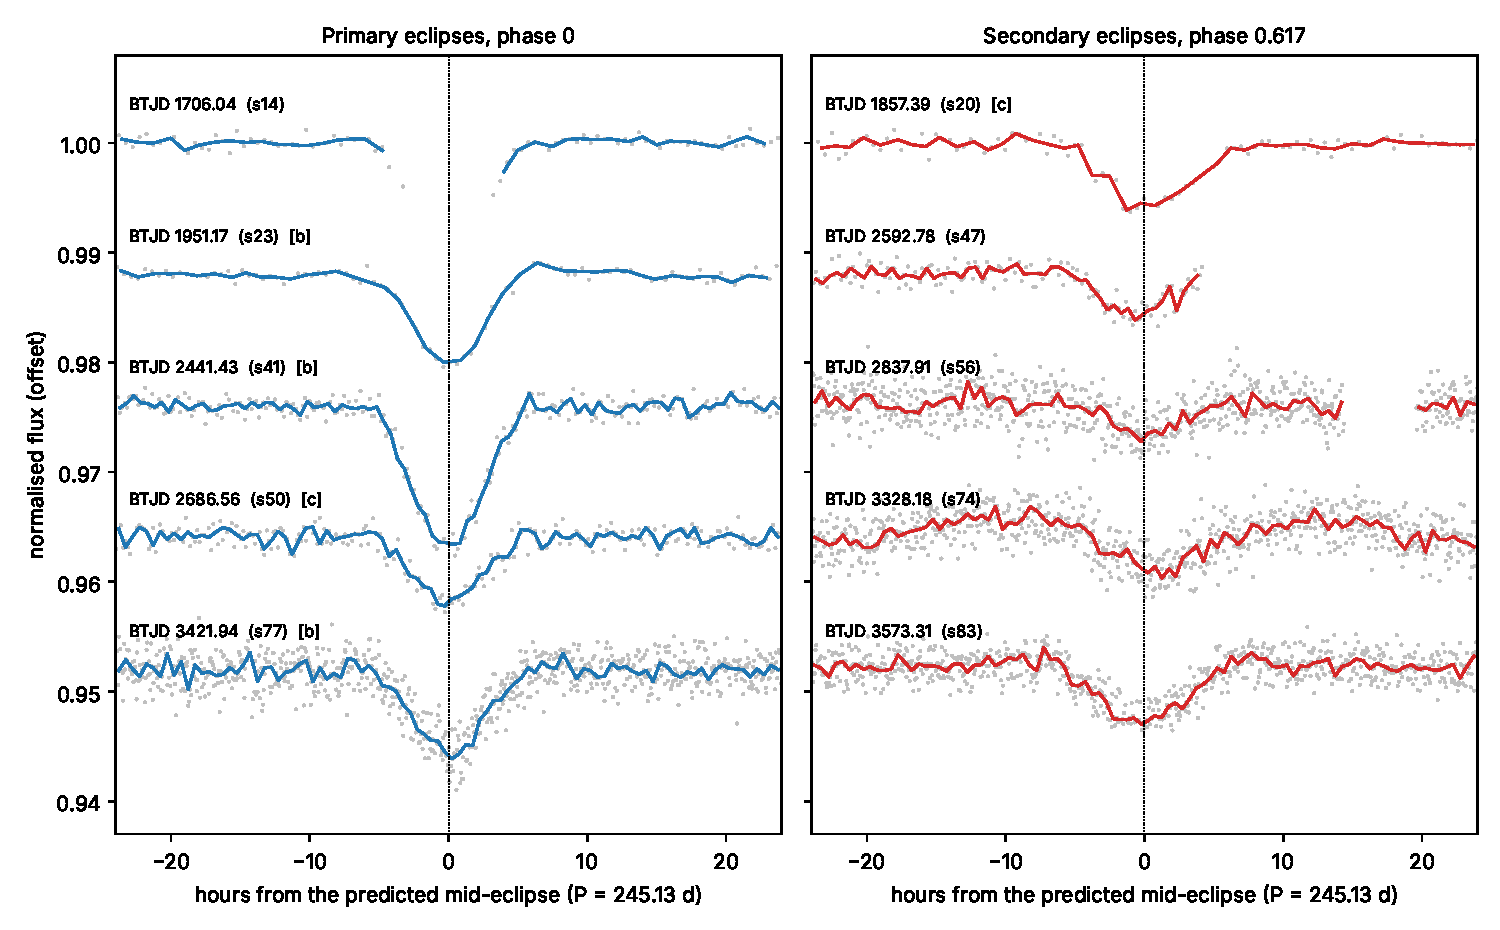
\includegraphics[width=\textwidth]{tic229701403_eclipses.pdf}
\caption{All ten eclipses, centred on the times predicted with
$P = 245.13$~d (pipeline light curves; lines: 30-min to 1-h bins). Left:
primary eclipses, right: secondary eclipses. The labels [b] and [c] mark the
events used by the two candidates. Sector 14 (top left) has a data gap
during the eclipse.}
\label{fig:t2297-ecl}
\end{figure}

\begin{figure}[ht]
\centering
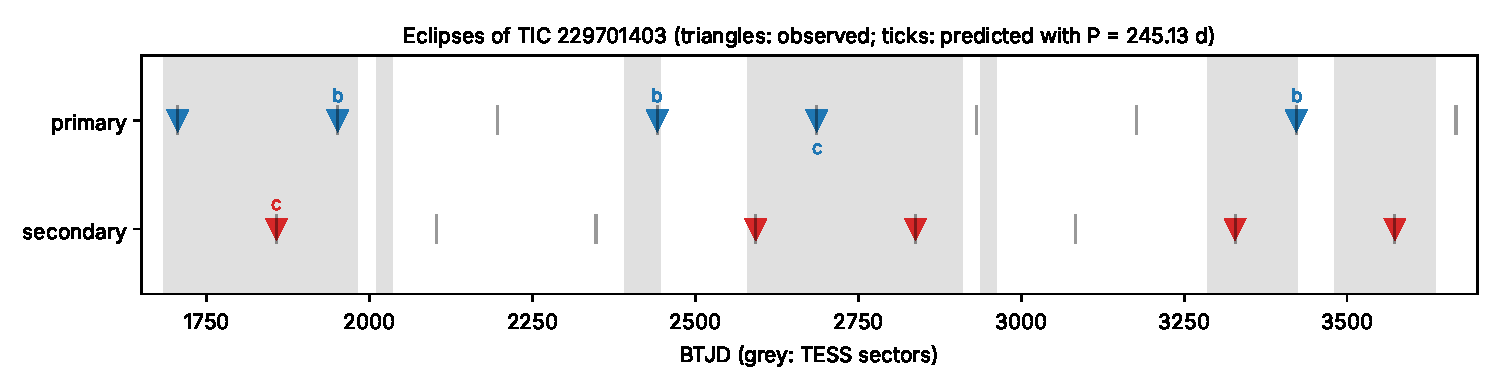
\includegraphics[width=\textwidth]{tic229701403_timeline.pdf}
\caption{Timeline: TESS sectors (grey), observed eclipses (triangles) and
the eclipses predicted with $P = 245.13$~d (ticks). Predicted eclipses
without a triangle fall in gaps between sectors.}
\label{fig:t2297-time}
\end{figure}

\section*{Where the eclipses happen}

The difference images put the source on TIC~229701402, 65$''$ from the
target. That star supplies only 2--4~\% of the light in the TESS aperture,
so to produce dips of 0.3--1~\% it must dim by 20--45~\%: these are
stellar eclipses, not transits. Two observations agree with this:

\begin{itemize}
\item \textbf{The depth changes from sector to sector.} The fraction of the
neighbour's light that falls in the aperture changes with the aperture and
the position of the star on the detector. A dip on the neighbour therefore
has a different depth in every sector; a dip on the target would not.
\item \textbf{The shape is V-like} (audit fold, b run): a grazing or partial
eclipse of two stars, not the flat-bottomed transit of a planet.
\end{itemize}

TRICERATOPS itself gives the neighbour scenarios (NEB, NEBx2P) a low
probability. It models one transit with one depth for all events, which a
signal of varying depth on a star at the edge of the aperture does not
fit. The difference imaging does not need that assumption, which is why
the audit treats its 30$\sigma$ offset as a FAIL.

\section*{What observers can do}

The decisive observation is a ground light curve with \emph{separate
apertures} on TIC~229701403 and TIC~229701402 during an eclipse: at 65$''$
the two stars are easily separated. The neighbour should show an eclipse of
tens of per cent, the target nothing. The star is circumpolar from Europe
(declination $+71.6^\circ$) and bright enough for small telescopes. The
next eclipses (allow $\pm1$~h around mid-eclipse; they last about 10~h):

\begin{center}
\begin{tabular}{@{}lll@{}}
\toprule
Eclipse & Mid-eclipse (BJD\_TDB) & Date (UTC, approx.)\\
\midrule
Primary & 2461402.45 & 27 December 2026, 23~h\\
Secondary & 2461553.80 & 28 May 2027, 07~h\\
Primary & 2461647.58 & 30 August 2027, 02~h\\
\bottomrule
\end{tabular}
\end{center}

Because the eclipse lasts longer than a night, partial coverage with a
good baseline on one side is enough to see a dip of this size. Light curves
in two bands (Section~\ref{sec:multiband}) add the colours of the two
eclipsed stars: the ratio of the primary and secondary depths in each band
gives their temperature ratio.

\begin{tip}
\textbf{Lessons.}
(1)~Several long-period candidates on one star: check whether all their
dips share a common period, with primaries and secondaries.
(2)~A predicted transit that is absent in data that cover it is a strong
sign that the period is wrong.
(3)~Large odd/even differences together with a secondary eclipse far from
phase 0.5 point to an eccentric eclipsing binary at twice (or a fraction
of) the assumed period.
(4)~A difference-image centroid that sits on another star in every sector
outweighs a low TRICERATOPS probability for that star.
(5)~The audit's own fold of these runs was at first a flat line: it read
two sectors that the pipeline had excluded for scattered light. Since
v4.3 the audit leaves out the same sectors as the pipeline and masks the
transits of masked candidates.
\end{tip}


%% ----------------------------------------------------------------------
\chapter{An M-dwarf candidate: L 279-94 (TIC 100796276)}
\label{ch:l27994}

L~279-94 is a nearby M dwarf (43.5~pc, $V = 13.9$, $T_\mathrm{mag} =
11.7$, declination $-53^\circ$) with a transit candidate reported by
P.~Rabtsevich in \emph{An 18-Day Planet Candidate around the Nearby Red
Dwarf L~279-94} (Zenodo, draft of 20~October 2026): an 18.152-day period,
a depth of 0.32~\%, a duration of 2.4~h and six TESS transits between 2020
and 2026, two of them predicted before the data were inspected. The note
is careful: it calls the signal a planet \emph{candidate}, because a
planet around a hidden companion star is still possible. Candidates around M dwarfs are
attractive because a small star makes a small planet easy to see, and
because their habitable zones lie at short periods. This chapter shows what
the pipeline concludes: why the candidate is not validated with the default
companion prior even though nothing argues against it, how it passes once
Gaia is used to limit the possible companions (MOLUSC), what that pass rests
on, and which observations would settle it.\footnote{Results of the runs of
6~November (pipeline v4.1.1), 19~November (v4.3, two identical runs, 10-min
bins) and 20~November 2026 (v4.3, 5-min bins; and 10-min bins with the
MOLUSC companions), all with TRICERATOPS+.}

\section*{Set-up}
The profile \code{profile_TIC100796276.json} gives the published ephemeris
(P = 18.15219~d, T0 = BTJD~2036.9763, 3200~ppm, 2.4~h) with a search of
$\pm3$~h around each predicted transit, the limb-darkened fit, the
neighbour vetting and the sensitivity test. TESS observed the star in five
sectors (27, 67, 94, 104, 105; full-frame images of 10 and 3.3~min). The
optimal apertures of 8--12 pixels hold 98.5--99.0~\% of the target's light;
the brightest neighbour within 2$'$ is 5.4~mag fainter
(Figure~\ref{fig:l279-field}).

\begin{figure}[ht]
\centering
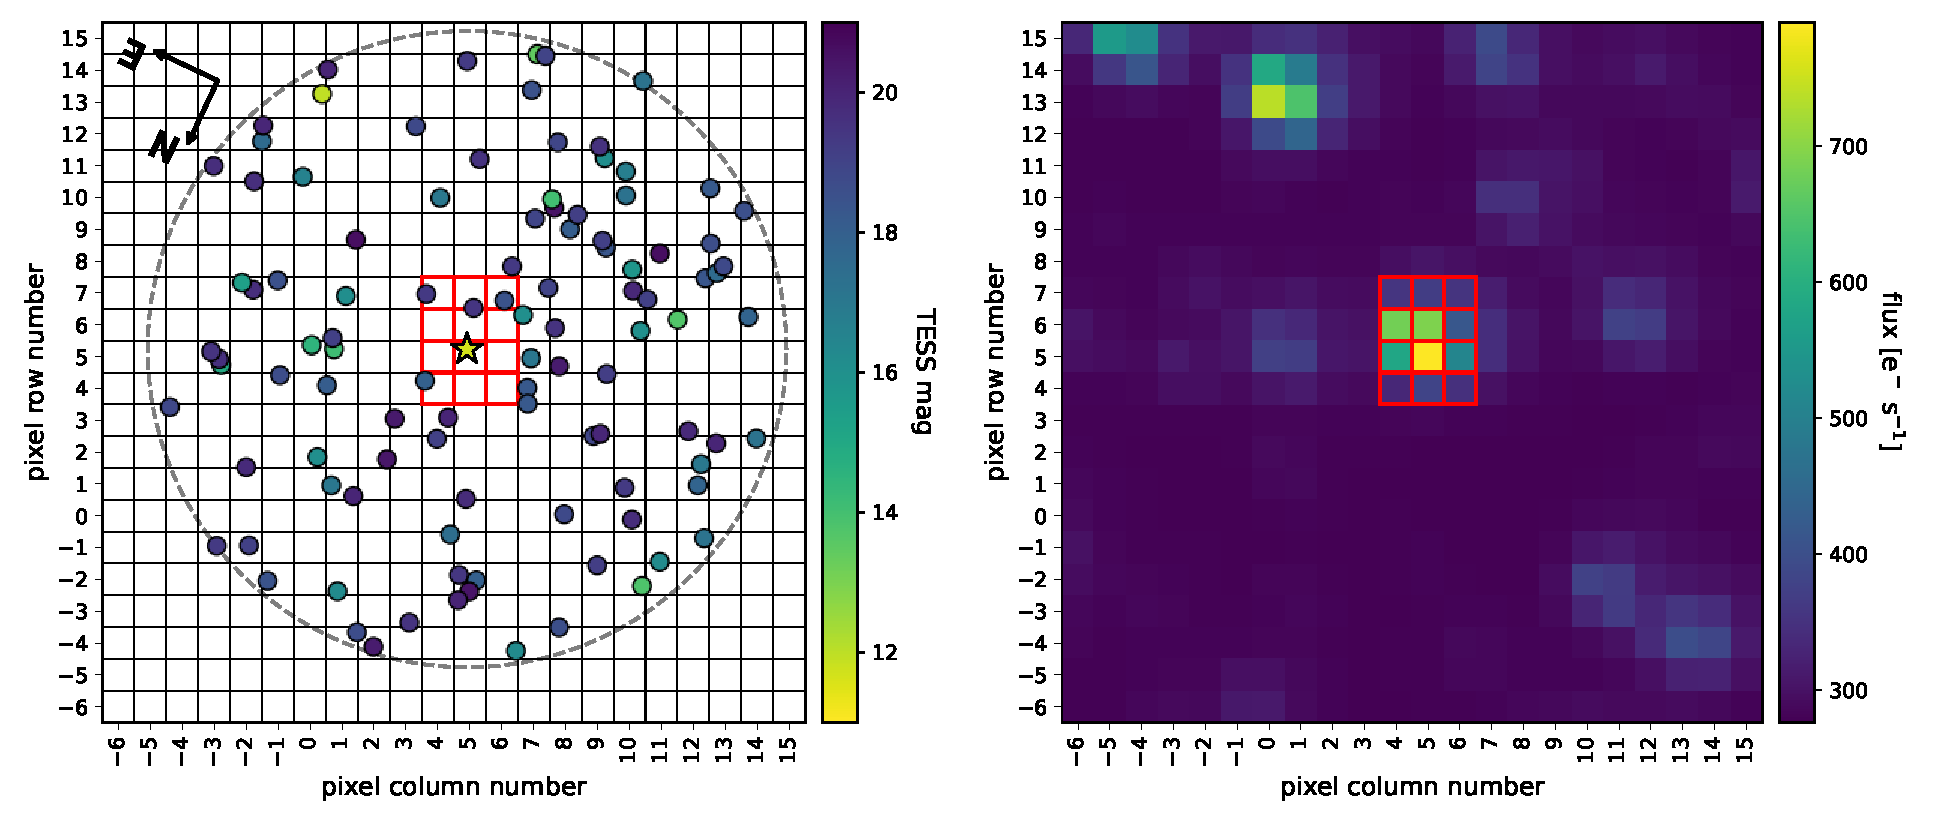
\includegraphics[width=0.8\textwidth]{l27994_field_s94.pdf}
\caption{Sector 94: TIC stars on the TESS pixel grid (left) and the image
with the optimal aperture (right). L~279-94 dominates its aperture.}
\label{fig:l279-field}
\end{figure}

\section*{Results}

\begin{longtable}{@{}p{0.38\textwidth}p{0.55\textwidth}@{}}
\toprule
\textbf{Quantity} & \textbf{Result}\\
\midrule\endhead
Star (TIC) & $T_\mathrm{eff} = 3491$~K, $R = 0.41~R_\odot$, $M = 0.40~M_\odot$\\
Transits & 7 in 5 sectors (one more than published; the one at the start
of sector 104 is weak, S/N 3)\\
Ephemeris & P = 18.15222~d, T0 = BTJD 2036.9718 (refined from the 7 transits)\\
Depth & 3690~ppm (limb-darkened fit), 3510~ppm on the target\\
Duration, shape & T14 = 2.36~h, U-shaped, not grazing; $R_p/R_\star = 0.057$\\
Planet radius & 2.5--2.8~$R_\oplus$: a sub-Neptune\\
Depth consistency & $\chi^2_\nu = 0.9$ over the 7 transits; odd/even 0.8$\sigma$\\
Secondary eclipse & none; 3$\sigma$ limit 525~ppm (a companion would be cooler than 2540~K)\\
Timing (ETV) & O$-$C rms 6.9~min, no significant trend\\
Stellar density & 11.9~g\,cm$^{-3}$ from the transit at $b = 0.32$, 8.2 from the TIC; $b$ is unconstrained ($\pm1.6$), so no conflict\\
Neighbours & the star at 41$''$ named in the Zenodo note (TIC~100795619)
is excluded by the difference imaging (6--8$\sigma$ from the centroid in
sectors 67 and 105); no other neighbour can produce the dip (NFPP = 0)\\
Difference imaging & centroid on the target (median 0.4$\sigma$, 3 of 5 sectors with enough S/N in v4.3)\\
FPP / NFPP, default companions & 0.036 $\pm$ 0.005 (10-min bins, three runs), 0.032 $\pm$ 0.004 (5-min bins) / 0\\
FPP / NFPP, Gaia-limited companions & 0.0070 $\pm$ 0.0015 / 0 (MOLUSC, 10-min bins)\\
Verdict & NOT passed with the default companion prior; PASSED with the companions Gaia still allows, under the assumption discussed below\\
\bottomrule
\end{longtable}

\begin{figure}[ht]
\centering
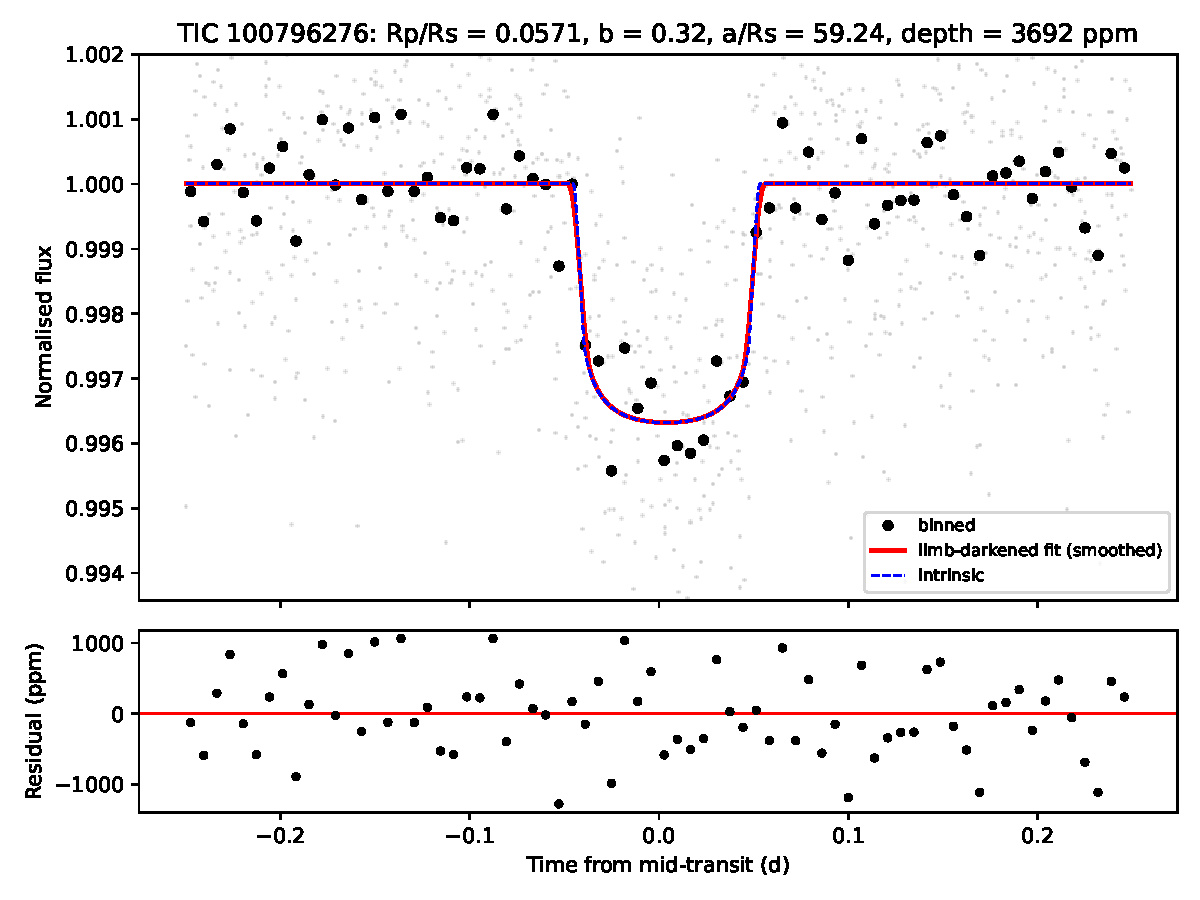
\includegraphics[width=0.49\textwidth]{l27994_ld_fit.pdf}\hfill
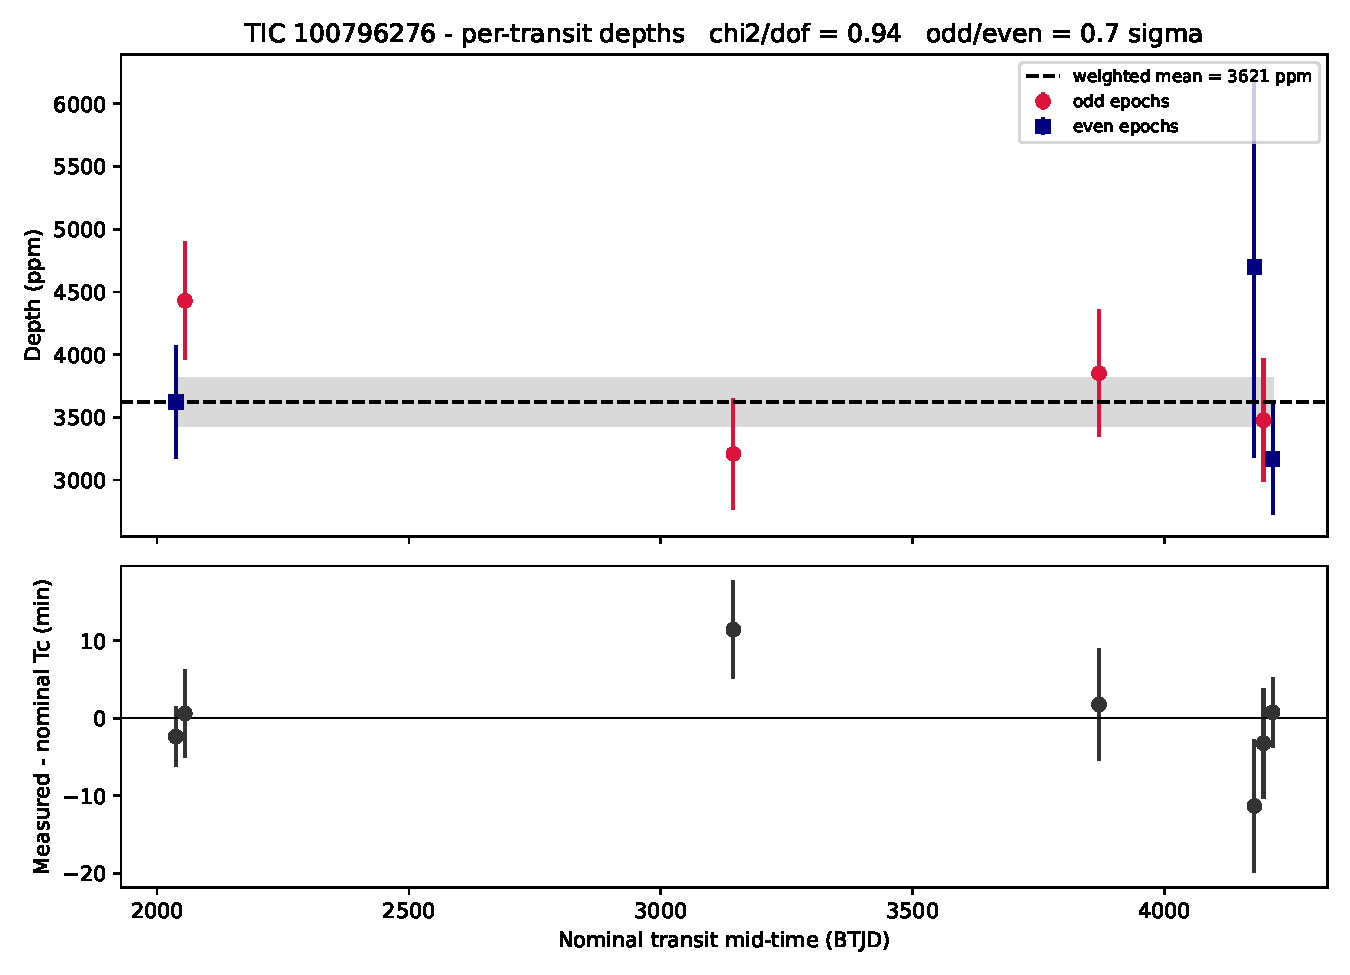
\includegraphics[width=0.49\textwidth]{l27994_per_transit.pdf}
\caption{Left: the seven transits folded, with the limb-darkened fit
(10-min bins). Right: depth and mid-time of each transit; odd (red) and even
(blue) agree.}
\label{fig:l279-fit}
\end{figure}

\section*{Comparison with the Zenodo note}

The two analyses are independent (other light curves, other code) and
agree on everything the light curve measures:

\begin{center}
\begin{tabular}{@{}p{0.27\textwidth}p{0.34\textwidth}p{0.32\textwidth}@{}}
\toprule
 & Rabtsevich (2026) & This pipeline\\
\midrule
Period & 18.15219 $\pm$ 0.00003~d & 18.15222~d\\
Depth, duration & 0.32~\%, 2.4~h & 0.35--0.37~\%, 2.36~h\\
Planet radius & 2.54 $\pm$ 0.10~$R_\oplus$ & 2.5--2.8~$R_\oplus$\\
Insolation & 2.4 $\times$ Earth & 2.3 $\times$ Earth\\
Transits & 6 (the 7th, at the start of sector 104 in stray light, left out) & 7 (the 7th weak, S/N 3)\\
Source of the dip & within $\sim$5$''$ of the star; TIC~100795619 very unlikely & centroid on the target; TIC~100795619 excluded\\
Secondary eclipse & none ($<$0.05--0.07~\%) & none ($<$0.05~\%)\\
FPP, default companions & 0.022 (TRICERATOPS 1.1.0) & 0.037 (TRICERATOPS+ 1.0.17)\\
FPP, companions limited by Gaia (MOLUSC) & 0.003--0.004 (passes) to 0.042 & 0.0070 $\pm$ 0.0015 (passes, 10-min bins)\\
\bottomrule
\end{tabular}
\end{center}

The note gives seven TRICERATOPS results under different assumptions. With
the default companion prior both analyses stay above the bar of 0.015. With
the companions that Gaia still allows (computed with MOLUSC, Wood et al.\
2021) the note's main analysis passes, but not with every treatment of the
data (10-min bins fail), and its second analysis fails. Two of its remarks
matter for this pipeline: the ingress of this planet lasts about 11~min,
so 10-min bins blur the shape of the transit; and TRICERATOPS 1.1.0 ignores
companions closer than about 3~au, the version used here does not, which
alone makes our FPP higher.

We therefore repeated the run with 5-min bins (\code{--bin-minutes 5},
profile \code{profile_TIC100796276_bin5}). The FPP changes from 0.036 to
0.032, within the run-to-run scatter: with the default companion prior the
bin width does not matter for this star. Two side effects of the shorter
bins taught us something. The free limb-darkened fit, now with more noise
per bin, jumped to a long, grazing solution ($b = 0.91$, T14 = 3.1~h)
that implies a stellar density of 0.9~g\,cm$^{-3}$, impossible for an M
dwarf of 0.4~$M_\odot$; since v4.3 such a fit is repeated with a prior on
the catalogue density (here: $b = 0.48$, T14 = 2.40~h). And the depth check
before TRICERATOPS used the three lowest bins of the fold, which noise makes
too deep; it now uses the median of the central bins. The note concludes,
as we do, that the candidate is not validated.

\section*{Why it is not validated}

Every test the light curve allows is passed. What remains is one scenario
that TESS cannot test: \textbf{STP}, the same planet transiting an
unresolved \emph{bound companion} of similar mass (best fit 0.36~$M_\odot$,
45~\% of the light). The probabilities of the last TRICERATOPS iteration are

\begin{center}
\begin{tabular}{@{}lll@{}}
\toprule
Planet on the target & TP 0.82, PTP 0.10, DTP 0.05 & 0.97\\
Planet on a bound companion & STP & 0.033\\
All eclipsing-binary scenarios & & $< 0.001$\\
\bottomrule
\end{tabular}
\end{center}

STP is a false positive in the sense of TRICERATOPS (the planet would not
orbit the target, and it would be larger, about 3.8~$R_\oplus$), and its
probability comes almost entirely from the \emph{prior}: M dwarfs often have
companions, and a twin companion leaves the light curve unchanged. This
also explains the sensitivity test:

\begin{center}
\begin{tabular}{@{}lcccc@{}}
\toprule
Noise $\times$ & 0.5 & 1 & 2 & 4\\
FPP, 6 Nov (v4.1.1) & 0.010 & 0.036 & 0.032 & 0.042\\
FPP, 19 Nov, run A (v4.3) & 0.055 & 0.037 & 0.033 & 0.043\\
FPP, 19 Nov, run B (v4.3) & 0.005 & 0.034 & 0.031 & 0.043\\
FPP, 20 Nov, 5-min bins (v4.3) & 0.559 & 0.034 & 0.030 & 0.042\\
\bottomrule
\end{tabular}
\end{center}

The FPP hardly depends on the assumed noise: it is set by the companion
prior, not by the quality of the light curve. Only the optimistic case
(half the measured noise) sometimes passes, which the audit flags as
\emph{not a validation}. The two identical runs of 19~November show why
that case cannot be trusted anyway: at half the noise the likelihoods are
sharper, the Monte-Carlo sampling noisier, and three pooled runs give 0.055
in one run and 0.005 in the other; with 5-min bins the same case even gives
0.56, because half the measured noise is then well below the white noise of
a bin (470 against 760~ppm) and no model fits. The nominal FPP, from 20 runs, is
reproducible to $\pm0.003$. More TESS data will not change this; an observation that
looks for companions will. The Zenodo note reaches the same point from the
other side: its FPP drops below 0.015 only when Gaia is used to limit the
companions.

\section*{With the companions Gaia still allows (MOLUSC)}

MOLUSC (Section~\ref{sec:molusc}) simulated $10^6$ possible companions of
L~279-94 and compared each with the Gaia DR3 astrometry (RUWE = 1.32) and
Gaia imaging (profile \code{profile_TIC100796276_molusc}, script
\code{MOLUSC/run_molusc_L27994.sh}). The survivors, by closest approach
to the star:

\begin{center}
\begin{tabular}{@{}lrrl@{}}
\toprule
Periastron & Survivors & of which $q > 0.75$ & used by TRICERATOPS\\
\midrule
$<$ 1~au & 205\,995 & 45\,578 & no\\
1--3~au & 58\,886 & 7\,760 & no\\
3--10~au & 47\,767 & 1\,704 & no\\
10--100~au & 85\,266 & 3\,852 & yes\\
$>$ 100~au & 67\,569 & 654 & yes\\
\midrule
All & 465\,483 (46.5~\%) & 59\,548 & 152\,835 (15.3~\%)\\
\bottomrule
\end{tabular}
\end{center}

Gaia excludes more than half of all companions. Beyond 10~au few
\emph{bright} ones remain (mass ratio $q > 0.75$, the near-twins that STP
needs): 4\,506 per million, against 45\,578 within 1~au. With these companions, and every star assumed to have one,
TRICERATOPS gives

\begin{center}
\begin{tabular}{@{}lcc@{}}
\toprule
 & default companions & Gaia-limited (MOLUSC)\\
\midrule
TP / PTP / DTP & 0.82 / 0.11 / 0.05 & 0.81 / 0.13 / 0.05\\
STP & 0.025--0.033 & 0.006\\
FPP (pooled, 20 runs) & 0.032--0.037 & 0.0070 $\pm$ 0.0015\\
FPP at 0.5 / 2 / 4 $\times$ the noise & 0.005--0.56 / 0.03 / 0.04 & 0.000 / 0.007 / 0.015\\
Verdict & NOT passed & PASSED\\
\bottomrule
\end{tabular}
\end{center}

and the audit has no FAIL (one WARN, the unconstrained impact parameter);
its \emph{Evaluation} names the companion prior. This agrees with the main
analysis of the Zenodo note (0.003--0.004).

\textbf{What the pass rests on.} The table shows the catch. Most surviving
near-twin companions (45\,578 of 59\,548) come closer than 1~au to the
star: Gaia cannot see them, and with no radial velocities nothing rules
them out. They do not count because TRICERATOPS uses only companions
beyond 10~au, on the grounds that planets are rare in close binaries. For
an 18-day planet at 0.1~au a companion within $\sim$0.4~au would make the
orbit unstable anyway, but between about 0.4 and 10~au planets are
suppressed, not forbidden. The Zenodo note's second analysis, which keeps
these companions, does not pass (FPP 0.030). The honest summary is
therefore: \emph{L~279-94~b passes the validation criteria when Gaia limits
the wide companions and planets are assumed absent in binaries closer than
10~au}. Spectroscopy, which sees exactly those close companions, would turn
the assumption into a measurement.

\section*{Is it in the habitable zone?}

The Zenodo note does not claim it is; it gives the insolation (2.4 times
the Earth's). The question comes up whenever a planet orbits an M dwarf, so
here is the comparison.


With the TIC parameters the star emits 2.3~\% of the Sun's luminosity and
the planet orbits at 0.100~au. It receives
$S = 2.3 \pm 0.5$ times the insolation of the Earth (more than Venus,
1.9), and its equilibrium temperature is 310--340~K (Bond albedo 0.3--0).
The habitable zone of this star (Kopparapu et al.\ 2014) begins at
$S = 1.5$ (optimistic inner edge, ``recent Venus'', P $\approx$ 25~d) and
the conservative zone lies between $S = 0.93$ and 0.25 (P = 35--96~d)
(Figure~\ref{fig:l279-hz}). The candidate is therefore a \emph{warm
sub-Neptune just inside the inner edge}, not a habitable-zone planet; and at
2.5--2.8~$R_\oplus$ it is most likely not rocky. A planet further out in
the same system could lie in the zone: 25--96~d periods are well within
reach of TESS and of ground photometry.

\begin{figure}[ht]
\centering
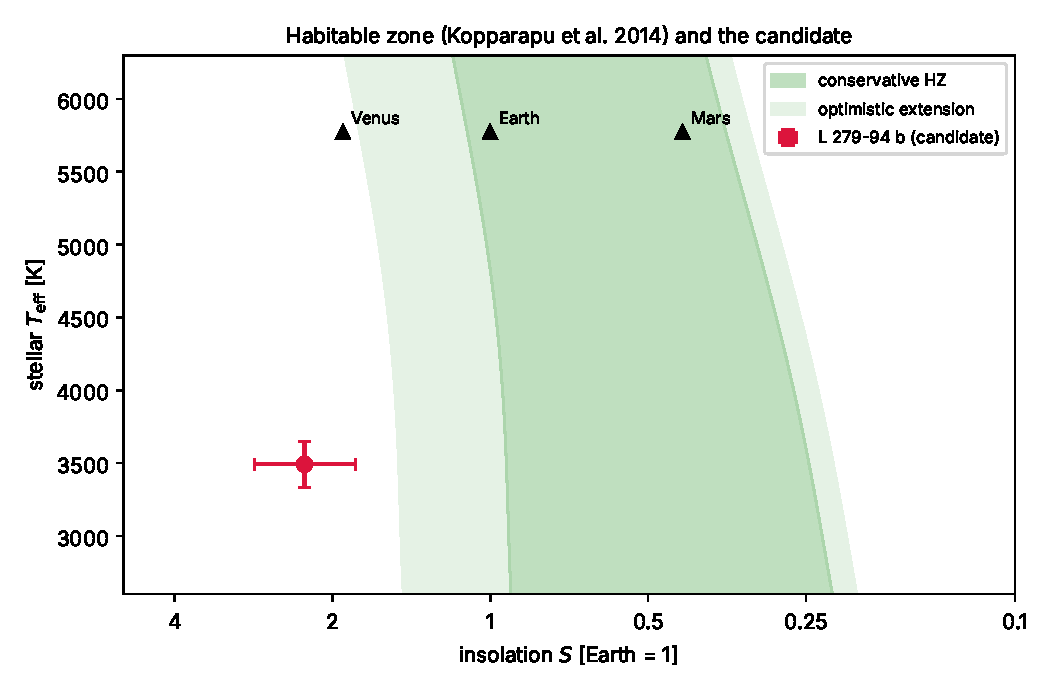
\includegraphics[width=0.7\textwidth]{l27994_hz.pdf}
\caption{Insolation of the candidate (red; error bar from the TIC
uncertainties of $T_\mathrm{eff}$ and radius) against the habitable zone
for main-sequence stars. Dark green: conservative zone (runaway to maximum
greenhouse); light green: optimistic extensions (recent Venus, early Mars).
Venus, Earth and Mars for comparison.}
\label{fig:l279-hz}
\end{figure}

\section*{What observers can do}

With the default companion prior the audit page \emph{Next observations}
ranks three observations, all aimed at the STP scenario. With MOLUSC the
criteria are already met; the same observations then test its assumptions,
and spectroscopy moves to the first place because it sees the close
companions that Gaia cannot:

\begin{enumerate}
\item \textbf{Transits in two bands} ($g'$ and $z'$, simultaneous if
possible). A planet on L~279-94 gives the same depth in both. On the
best-fit companion (about 3140~K, cooler than the target) the depth in $g'$
would be only 0.77 times that in $z'$: about 930~ppm apart, visible at
3$\sigma$ with a depth error of $\leq$310~ppm per band. The audit estimates
that a typical result brings the FPP to 0.007 --- enough on its own.
Several transits per band can be combined; TRICERATOPS+ uses them directly
(Section~\ref{sec:multiband}), and the audit's \emph{Multi-band} test then
states which scenarios they exclude.
\item \textbf{High-resolution imaging} (speckle, adaptive optics): at
43.5~pc, 0.1$''$ is 4.4~au, so most bound companions would be resolved.
Typical outcome FPP 0.017; give the contrast curve to the pipeline with
\code{--contrast-curve}.
\item \textbf{Reconnaissance spectroscopy}: a companion with 45~\% of the
light shows a second set of lines. Typical outcome FPP 0.011.
\end{enumerate}

According to the Zenodo note, Gaia DR4 (scheduled for 2~December 2026)
will add five and a half years of astrometry, which can reveal companions
directly; MOLUSC should then be rerun with the
new values.

\textbf{Practical.} The transit is 3.5~ppt deep and lasts 2.4~h; with
$V = 13.9$ but $T \approx I \approx 11.7$ the star is much brighter in the red, so
$z'$ (or I) gives the best precision and $g'$ (or V) is the demanding band.
At declination $-53^\circ$ it is a southern-hemisphere target, best
observed from June to September. Predicted mid-transits (formal error
$\pm7$~min; observe at least 1~h before and after):

\begin{center}
\begin{tabular}{@{}lll@{}}
\toprule
Mid-transit (BJD\_TDB) & UTC (approx.) & Night side\\
\midrule
2461560.131 & 2027 June 3, 15:07 & Australia\\
2461578.283 & 2027 June 21, 18:47 & Australia (morning)\\
2461596.435 & 2027 July 9, 22:26 & South Africa\\
2461614.587 & 2027 July 28, 02:05 & South America, South Africa\\
2461632.739 & 2027 August 15, 05:44 & South America\\
2461669.044 & 2027 September 20, 13:03 & Australia\\
\bottomrule
\end{tabular}
\end{center}

The GUI tool \emph{Predicted transit times} gives the times for any
date range (Section~\ref{sec:tools}). The Zenodo note predicts the
transits of 4 and 22~December 2026 at 02:40 and 06:20~UTC ($\pm3$~min);
our ephemeris gives 02:35 and 06:15 ($\pm7$~min): consistent.

\begin{tip}
\textbf{Lessons.}
(1)~A clean light curve is not a validation: when every test passes and
the FPP stays at a few per cent, look at \emph{which} scenario holds it.
(2)~If the FPP barely changes with the assumed noise, it is set by a prior
(here: bound companions of M dwarfs), and only an observation that tests
that prior can lower it.
(3)~``Habitable zone'' needs a number: compute the insolation from the
stellar luminosity and the orbit, and compare with the zone of a star of
that temperature.
(4)~The FPP of a candidate like this depends on modelling choices
(companion prior, bin width, TRICERATOPS version): report it with the
choices, as the Zenodo note does, and test the obvious alternatives
(\code{--bin-minutes 5}, \code{--molusc-file}).
(5)~Repeat a run before trusting a number that sits near a threshold: two
identical runs are the cheapest test of Monte-Carlo noise
(\code{--sens-runs} raises the number of runs per sensitivity case).
(6)~Gaia (through MOLUSC) can turn a ``not validated'' into ``validated''
without telescope time, but only for the companions Gaia could have seen;
state the companion model and what it assumes about close binaries.
\end{tip}


%% ----------------------------------------------------------------------
\chapter{Other useful functions}

\begin{description}
\item[Import a command line.] \emph{File $\rightarrow$ Import command
line}: paste a command, from a colleague or from the technical manual, and
the fields are filled in.
\item[Copy command.] To run the same analysis in a terminal or on another
computer.
\item[New.] Resets all options.
\item[Last session.] Saved automatically in \code{~/.triceratops_gui.json}.
\item[Regression tests.] \emph{Tools $\rightarrow$ Run regression tests}
checks the installation in the selected interpreter (about 30 tests,
$\sim$1~min).
\item[Manuals.] \emph{Help $\rightarrow$ Observer's Guide (PDF)} opens this guide, \emph{Help $\rightarrow$ Technical manual (PDF)} the full technical manual.
\item[Audit.] \emph{Results $\rightarrow$ Audit run}, or \emph{Tools
$\rightarrow$ Audit output folder} for the current target, or \emph{Audit
another output folder\ldots} for an older run (Chapter~\ref{ch:followup}).
\item[Batch runs.] \code{triceratops_batch.py} (by Steve Price) runs a list of
candidates from a JSON file: \code{--mode prefetch} downloads all TESScut
cutouts first, \code{--mode test} then runs the pipeline and the audit for
each, a few at a time. See \code{examples/batch_example.json}.
\end{description}

%% ----------------------------------------------------------------------
\chapter{Kepler targets}
\label{ch:kepler}

Since v4.2 the same analysis runs on Kepler data (2009--2013). Choose
\emph{Mission = kepler} and give the \emph{KIC ID} (Figure~\ref{fig:kepler}).

\begin{figure}[ht]
\centering
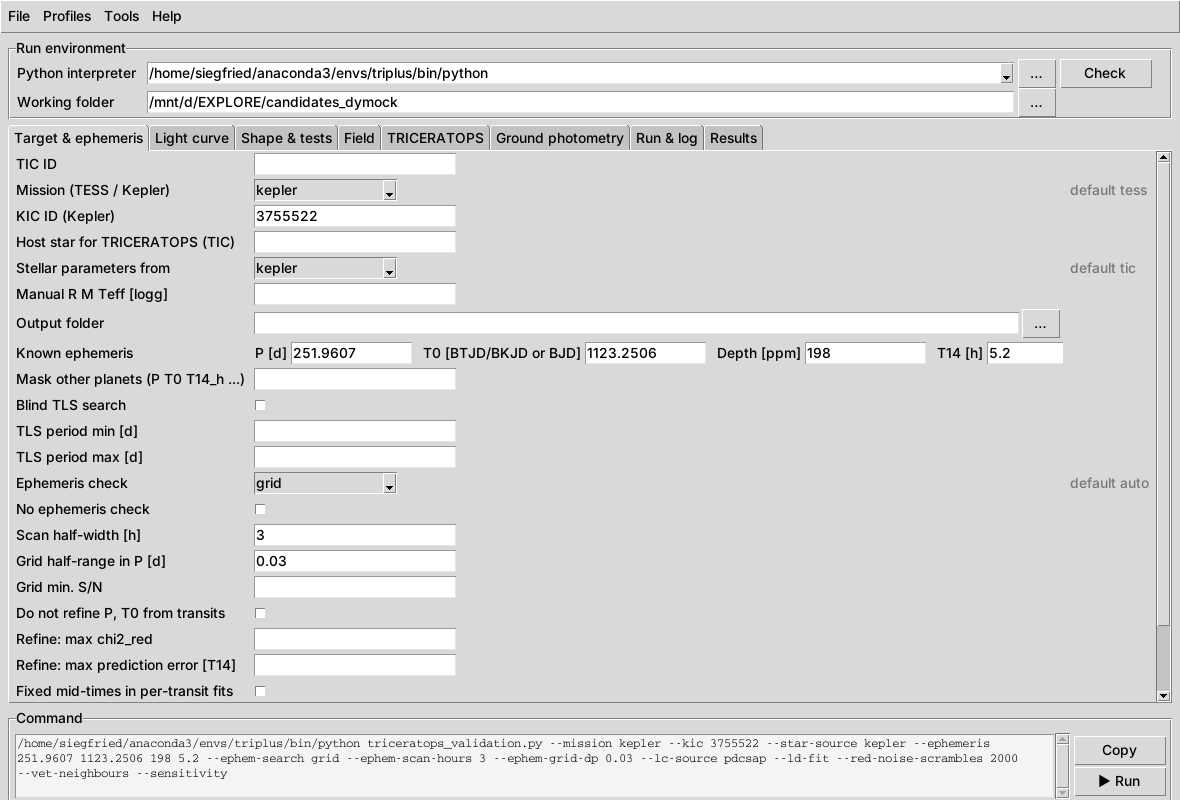
\includegraphics[width=\textwidth]{og_tab_kepler.png}
\caption[Kepler profile]{Profile \texttt{profile\_KIC3755522} (KOI-5005.01, Rabtsevich 2026):
Kepler mode, KIC~3755522, stellar parameters from the Kepler catalogues.}
\label{fig:kepler}
\end{figure}

\begin{itemize}
\item \textbf{Data.} Long-cadence (29.4~min) PDCSAP or SAP light curves and
target pixel files per quarter; the quarters take the place of the sectors.
\item \textbf{Times} are in BKJD = BJD\_TDB $-$ 2454833 (TESS: BTJD =
BJD\_TDB $-$ 2457000). A known T0 may also be given as the full BJD.
\item \textbf{TIC number.} TRICERATOPS still needs the TIC for the field
stars. The pipeline looks it up from the KIC. Old TIC entries of close pairs
are often flagged SPLIT or DUPLICATE; the pipeline then takes the star at the
KIC position, prints all candidates within 4$''$, and removes the flagged
entries from the TRICERATOPS star table. Check the list in the log; with
\code{--tic} you choose another star.
\item \textbf{Stellar parameters.} \emph{Stellar parameters from = kepler}
takes them from Berger et al.\ (2020, Gaia--Kepler), else from the DR25
stellar table (Mathur et al.\ 2017).
\item \textbf{Host.} For a close pair such as KIC~3755522~A and B
(2.49$''$) give the TIC of B as \emph{Host star} and its parameters under
\emph{Manual R M Teff} to ask whether a planet on B explains the signal.
\item \textbf{VizieR.} When \code{vizier.cds.unistra.fr} cannot be reached
the pipeline uses a mirror (CfA, IUCAA, NAO) and says so in the log.
\end{itemize}

Command-line equivalent of the profile:
\begin{lstlisting}
triceratops_validation.py --mission kepler --kic 3755522 --star-source kepler --ephemeris 251.9607 1123.2506 198 5.2 --ephem-search grid --ephem-scan-hours 3 --ephem-grid-dp 0.03 --lc-source pdcsap --ld-fit --vet-neighbours --sensitivity
\end{lstlisting}

%% ======================================================================
\part{Reference}
%% ======================================================================

\chapter{All options}
\label{ch:options}

The tables list every option of \code{triceratops_validation.py} v4.3,
grouped as on the tabs of the GUI. They were generated from the script
itself. ``--'' means that the script chooses the value itself, as described
in the explanation. In the GUI, leave such a field empty.

\begin{tip}
\textbf{The options most observers need:} TIC ID (or Mission and KIC),
known ephemeris, scan half-width, limb-darkened fit, ground light curves, and
for TRICERATOPS+ the dilution correction \emph{none} with the aperture depth.
Everything else can stay at its default.
\end{tip}

\small
\subsection*{Tab: Target \& ephemeris}
\begin{longtable}{@{}p{0.2\textwidth}p{0.22\textwidth}p{0.1\textwidth}p{0.4\textwidth}@{}}
\toprule \textbf{GUI field} & \textbf{Command line} & \textbf{Default} & \textbf{Meaning}\\ \midrule\endhead
TIC ID & \code{--tic TIC} & required & TIC ID of the target (Kepler mode: looked up from \code{--kic} when not given).\\
Mission (TESS / Kepler) & \code{--mission tess|kepler} & tess & tess (default) or kepler: Kepler long-cadence light curves and pixel files per quarter; times in BKJD (BJD - 2454833); needs \code{--kic}.\\
KIC ID (Kepler) & \code{--kic KIC} & -- & Kepler Input Catalog number (with \code{--mission} kepler).\\
Host star for TRICERATOPS (TIC) & \code{--host-tic TIC} & -- & Star that TRICERATOPS treats as the host (e.g. a close companion); the light curve and pixels stay those of \code{--tic} / \code{--kic}.  The light curve is then used on the aperture scale (SAP,\allowbreak{} no dilution correction).\\
Stellar parameters from & \code{--star-source tic|kepler} & tic & Host-star R,\allowbreak{} M,\allowbreak{} Teff,\allowbreak{} logg: tic (default) or kepler (Berger et al. 2020 Gaia-Kepler catalogue,\allowbreak{} else the Kepler DR25 stellar table; needs \code{--kic}).\\
Manual R M Teff [logg] & \code{--stellar X ...} & -- & Manual host-star parameters R[Rsun] M[Msun] Teff[K] [logg]; override \code{--star-source}.\\
Output folder & \code{--outdir OUTDIR} & -- & Output directory (default: TIC\{tic\}/ in the CWD). Created automatically if missing.\\
Known ephemeris & \code{--ephemeris P_D T0_BTJD DEPTH_PPM T14_H} & -- & Known ephemeris for THIS target (skips the TLS search): period [d],\allowbreak{} T0 [BTJD; BKJD with \code{--mission} kepler; or the full BJD\_TDB],\allowbreak{} depth [ppm],\allowbreak{} duration [h].\\
Mask other planets (P T0 T14\_h ...) & \code{--mask-ephemeris X ...} & -- & Mask the transits of other known planets in the system: P T0 T14\_H for each (repeat the three values for more planets; T0 as for \code{--ephemeris}).  Cadences within 0.75 x T14 of their mid-times are removed.\\
Blind TLS search & \code{--blind-search} & off & Force a blind TLS search (default when \code{--ephemeris} is not given).\\
TLS period min [d] & \code{--p-min D} & -- & TLS period\_min [d] (default: 0.5).  Narrow the grid when you know the approximate period.\\
TLS period max [d] & \code{--p-max D} & -- & TLS period\_max [d] (default: 100,\allowbreak{} also clipped to baseline/n\_transits\_min at runtime).\\
Ephemeris check & \code{--ephem-search auto|scan|grid|off} & auto & With \code{--ephemeris}: how to check/refine P and T0 before detrending. scan = box search of each transit + robust linear fit; grid = folded box search on a (P,\allowbreak{} T0) grid (stacks all transits,\allowbreak{} for shallow signals); auto = scan,\allowbreak{} grid if the scan is inconclusive (default); off = keep the input.\\
No ephemeris check & \code{--no-ephem-scan} & off & Same as \code{--ephem-search} off.\\
Scan half-width [h] & \code{--ephem-scan-hours H} & -- & Half-width of the search in T0 [h],\allowbreak{} for scan and grid (default: max(2 x T14,\allowbreak{} 12 h)).\\
Grid half-range in P [d] & \code{--ephem-grid-dp D} & -- & Grid search: half-range in P [d] (default: the T0 half-range divided by the number of epochs from the reference epoch).\\
Grid min. S/N & \code{--ephem-grid-min-snr X} & -- & Grid search: minimum stacked S/N to adopt the result (default 7).\\
Do not refine P, T0 from transits & \code{--no-refine-ephemeris} & off & Do not refine P and T0 from the individual transit mid-times.\\
Refine: max chi2\_red & \code{--refine-chi2-max X} & -- & Max chi2\_red of the linear timing fit before the refined ephemeris is rejected (default: 8).  Raise for long-period targets with few transits.\\
Refine: max prediction error [T14] & \code{--ephem-adopt-max-sigma F} & -- & A refined ephemeris is adopted only if it predicts every epoch with data to within F x T14 (1 sigma; default 0.25).\\
Fixed mid-times in per-transit fits & \code{--no-tc-fit} & off & Keep the mid-time of each individual transit fixed at the ephemeris value.\\
\bottomrule\end{longtable}
\subsection*{Tab: Light curve}
\begin{longtable}{@{}p{0.2\textwidth}p{0.22\textwidth}p{0.1\textwidth}p{0.4\textwidth}@{}}
\toprule \textbf{GUI field} & \textbf{Command line} & \textbf{Default} & \textbf{Meaning}\\ \midrule\endhead
Light-curve source & \code{--lc-source tesscut|sap|pdcsap} & tesscut & Photometry: tesscut (FFI custom aperture,\allowbreak{} default),\allowbreak{} sap (SPOC SAP),\allowbreak{} or pdcsap (SPOC PDC). For sap/pdcsap the SPOC TPF is still fetched when available.\\
TESScut cache folder & \code{--download-dir DOWNLOAD_DIR} & -- & TESScut / SPOC cache directory (default: \textless{}outdir\textgreater{}/tesscut\_cache). Already-downloaded products are reused.\\
Only download the cutouts (no analysis) & \code{--prefetch-only} & off & Only download the TESScut cutouts this run would read (every sector,\allowbreak{} every cutout size) into the cache,\allowbreak{} then stop. Use with \code{--download-dir} to prepare runs in advance.\\
MAST timeout [s] & \code{--net-timeout NET_TIMEOUT} & 300.0 & Seconds a MAST request or TESScut download may wait for data before it is abandoned and retried (0: no limit,\allowbreak{} as astroquery). Default 300.\\
MAST attempts & \code{--net-retries NET_RETRIES} & 4 & Attempts for each MAST query and TESScut download,\allowbreak{} with pauses of 30,\allowbreak{} 60,\allowbreak{} 90 s ... between them. Default 4.\\
Exclude sectors & \code{--exclude-sectors S ...} & -- & Sector numbers to drop before extraction (e.g. \code{--exclude-sectors} 56 79).\\
No automatic sector exclusion & \code{--no-auto-exclude-sectors} & off & Do not auto-drop sectors that fail normalisation quality cuts after detrending.\\
Max sector rms & \code{--sector-max-rms SECTOR_MAX_RMS} & -- & Max robust RMS of norm\_flux (fractional; default 0.02).\\
Aperture & \code{--aperture optimal|percentile} & optimal & TESScut aperture: S/N-optimal from a catalogue PSF model (default) or pixels above the 85th percentile.\\
Dilution correction & \code{--dilution-mode sector|none} & sector & sector (default): put every sector on the target's flux scale with its own target fraction before folding; none: keep raw aperture flux.\\
Raw aperture flux & \code{--raw-aperture-flux} & off & Pass dilution\_corrected=False to triceratops (flux is an uncorrected aperture LC). Needs triceratops \textgreater{}= 1.1.\\
Light curve is dilution corrected & \code{--dilution-corrected} & off & Tell TRICERATOPS the light curve is crowding-corrected (automatic with \code{--dilution-mode} sector and for pdcsap).\\
Detrend windows [d] & \code{--detrend-windows D ...} & -- & First-pass biweight windows [d]; the blind TLS search runs once per window and the highest-SDE candidate is kept (e.g. 0.75 1.0 1.5 2.5).\\
Error floor [ppm] & \code{--err-floor-ppm ERR_FLOOR_PPM} & 0.0 & Lower bound on the flux uncertainty given to calc\_probs [ppm].\\
Do not inflate sigma & \code{--no-inflate} & off & Do not inflate sigma to chi2\_red = 1 of the reference model.\\
\bottomrule\end{longtable}
\subsection*{Tab: Shape \& tests}
\begin{longtable}{@{}p{0.2\textwidth}p{0.22\textwidth}p{0.1\textwidth}p{0.4\textwidth}@{}}
\toprule \textbf{GUI field} & \textbf{Command line} & \textbf{Default} & \textbf{Meaning}\\ \midrule\endhead
Limb-darkened fit & \code{--ld-fit} & off & Fit the folded LC with a limb-darkened transit model (u1,\allowbreak{}u2 fixed to the Claret values of the TIC/TLS catalogue) and use it as reference model for the sigma inflation.\\
LD coefficients free & \code{--ld-free} & off & Like \code{--ld-fit},\allowbreak{} but fit the limb-darkening coefficients (Kipping q1,\allowbreak{}q2).\\
LD coefficients u1 u2 & \code{--ld-coeffs U1 U2} & -- & Like \code{--ld-fit},\allowbreak{} with fixed quadratic coefficients.\\
No secondary-eclipse search & \code{--no-secondary-search} & off & Skip the secondary-eclipse search at all phases.\\
Secondary min. S/N & \code{--secondary-min-snr X} & -- & Stacked S/N for a secondary-eclipse detection (default 7).\\
Red-noise scrambles & \code{--red-noise-scrambles N} & 0 & Phase-randomisation trials for a red-noise false-alarm p-value on the stacked depth (0 disables; try 1000–5000).\\
Red-noise seed & \code{--red-noise-seed RED_NOISE_SEED} & 42 & RNG seed for \code{--red-noise-scrambles}.\\
No timing analysis & \code{--no-etv} & off & Skip the eclipse-timing / depth-variation analysis.\\
Extra mid-times file & \code{--extra-times FILE} & -- & Ground-based mid-times to add to the timing analysis: 'BJD\_TDB err\_min [label]' per line.\\
\bottomrule\end{longtable}
\subsection*{Tab: Field}
\begin{longtable}{@{}p{0.2\textwidth}p{0.22\textwidth}p{0.1\textwidth}p{0.4\textwidth}@{}}
\toprule \textbf{GUI field} & \textbf{Command line} & \textbf{Default} & \textbf{Meaning}\\ \midrule\endhead
Contrast curve & \code{--contrast-curve FILE} & -- & High-resolution imaging contrast curve: separation [arcsec],\allowbreak{} delta mag.\\
Vet neighbours & \code{--vet-neighbours} & off & Vet nearby stars from their own TESS light curves and exclude those that cannot host the signal.\\
No difference imaging & \code{--no-difference-imaging} & off & Skip the difference-image centroid analysis.\\
Exclude stars (TIC) & \code{--exclude-stars TIC ...} & -- & Stars cleared by other follow-up (removed before calc\_probs).\\
\bottomrule\end{longtable}
\subsection*{Tab: TRICERATOPS}
\begin{longtable}{@{}p{0.2\textwidth}p{0.22\textwidth}p{0.1\textwidth}p{0.4\textwidth}@{}}
\toprule \textbf{GUI field} & \textbf{Command line} & \textbf{Default} & \textbf{Meaning}\\ \midrule\endhead
Min. runs (n\_iter) & \code{--n-iter N_ITER} & 20 & Minimum number of TRICERATOPS calc\_probs runs (more are added until converged).\\
Samples per run (N) & \code{--n-samples N} & -- & Monte-Carlo draws per scenario in calc\_probs (default: triceratops default,\allowbreak{} 1e6). Raise when the log reports that the evidence is dominated by one run.\\
Do not pool runs & \code{--no-pool} & off & Do not pool the scenario evidences over the runs; report the mean of the per-run FPPs instead.\\
Sensitivity runs & \code{--sensitivity} & off & Also report FPP/NFPP at several flux-uncertainty scales (extra calc\_probs runs).\\
Runs per sensitivity case & \code{--sens-runs SENS_RUNS} & 3 & calc\_probs runs per scale for \code{--sensitivity} (pooled).\\
Model exposure [min] & \code{--tri-exptime-min M} & -- & Exposure smoothing of the TRICERATOPS models [min] (default: bin width + native cadences; 0 = package default of 2 min).\\
Max. runs & \code{--tri-max-iter N} & -- & Maximum calc\_probs runs while not converged (default 3 x \code{--n-iter}).\\
Time budget [s] & \code{--tri-time-budget S} & -- & Time budget for the extra runs [s] (default 3600).\\
TRILEGAL / field-star file & \code{--trilegal-fname TRILEGAL_FNAME} & -- & Pre-downloaded TRILEGAL table for triceratops (skips the SSL-sensitive online query).\\
TRICERATOPS+ & \code{--tri-plus auto|on|off} & auto & Pass ground light curves to calc\_probs when the installed triceratops is TRICERATOPS+ (auto,\allowbreak{} default),\allowbreak{} require it (on) or never (off).\\
Verdict from FPP/NFPP only (ignore own EB tests) & \code{--no-eb-veto} & off & Let the verdict depend on FPP/NFPP only,\allowbreak{} even when the pipeline detects a secondary eclipse,\allowbreak{} an odd/even difference or an absent parity.\\
Imaging inner working angle for advice ["] & \code{--hires-iwa ARCSEC} & -- & Inner working angle of high-resolution imaging in the observation recommendations (default 0.1).\\
\bottomrule\end{longtable}
\subsection*{Tab: Ground photometry}
\begin{longtable}{@{}p{0.2\textwidth}p{0.22\textwidth}p{0.1\textwidth}p{0.4\textwidth}@{}}
\toprule \textbf{GUI field} & \textbf{Command line} & \textbf{Default} & \textbf{Meaning}\\ \midrule\endhead
Ground light curves & \code{--ground-lc SPEC} & -- & Ground-based light curve (repeatable): 'path,\allowbreak{}band=r,\allowbreak{}star=TIC,\allowbreak{}ap=4.0,\allowbreak{}fwhm=2.5,\allowbreak{}obs=CODE,\allowbreak{}detrend=poly1,\allowbreak{}AIRMASS'. band: B V R I g r i z J H K (Rc=R,\allowbreak{} Sloan r'=r); star: TIC at the aperture centre (default: target); ap: aperture RADIUS [arcsec]; fwhm: seeing [arcsec]; time=BJD\_TDB (default) | JD\_UTC | HJD\_UTC; fcol/ecol/tcol: column names; mag=1 for magnitudes.\\
Ground list file & \code{--ground-list FILE} & -- & File with one \code{--ground-lc} specification per line (paths relative to that file).\\
Do not remove cleared stars & \code{--ground-no-clear} & off & Report the ground clearance but do not remove stars from TRICERATOPS.\\
Mid-time window [min] & \code{--ground-tc-window MIN} & -- & Minimum half-width of the ground mid-time search [min] (default 60; widened to 3 sigma of the TESS ephemeris).\\
Detection S/N & \code{--ground-min-snr GROUND_MIN_SNR} & -- & Detection threshold for ground light curves (default 5).\\
Depth tolerance & \code{--ground-depth-tol GROUND_DEPTH_TOL} & -- & Fractional tolerance on the expected ground depth (default 0.25).\\
Default seeing ["] & \code{--ground-fwhm ARCSEC} & -- & Seeing FWHM used when a light curve gives none (default 3.0).\\
\bottomrule\end{longtable}
\normalsize

\section*{Keys of a ground light-curve specification}
In the GUI these are the fields of the dialog. On the command line they are
written as \code{--ground-lc "file,band=R,star=65344134,ap=3.5,fwhm=2.4"}.

\begin{longtable}{@{}p{0.2\textwidth}p{0.73\textwidth}@{}}
\toprule
\textbf{Key} & \textbf{Meaning}\\
\midrule\endhead
\code{band} & B V R I (Johnson--Cousins; Rc = R), g r i z (Sloan; \code{r'}, \code{SR}, \code{rp} accepted), J H K, CBB, CV.\\
\code{star} & TIC at the aperture centre (default: target).\\
\code{ap}, \code{fwhm} & Aperture radius and seeing FWHM [arcsec].\\
\code{obs} & Observer.\\
\code{time} & \code{BJD_TDB} (default), \code{JD_UTC}, \code{HJD_UTC}.\\
\code{tcol}, \code{fcol}, \code{ecol} & Column names of time, flux, error.\\
\code{mag} & \code{1}: magnitudes.\\
\code{detrend} & \code{auto}, \code{poly0/1/2}, \code{none}, plus covariate columns.\\
\code{ra}, \code{dec} & Aperture centre [deg] instead of a star.\\
\code{pixscale} & [arcsec/pixel], to convert AstroImageJ radii.\\
\code{plus} & Band for TRICERATOPS+ (g r i z J H K).\\
\code{label} & Name in the log and figures.\\
\bottomrule
\end{longtable}

%% ----------------------------------------------------------------------
\chapter{Output files}

All files are written to the output folder (default \code{TIC<tic>/}, in
Kepler mode \code{KIC<kic>/}).

\begin{longtable}{@{}p{0.4\textwidth}p{0.53\textwidth}@{}}
\toprule
\textbf{File} & \textbf{Content}\\
\midrule\endhead
\code{triceratops_output_TIC<tic>.txt} & The complete log, ending with the SUMMARY block.\\
\code{summary_<tic>.json} & Key results (shown on the tab \emph{Results}).\\
\code{tesscut_<tic>_sNN.pdf}, \code{field_<tic>_sNN.pdf} & Cutout, aperture and field per sector.\\
\code{lc_panels_*_<tic>.pdf}, \code{lc_transits_sectors_<tic>.pdf} & Light curves per sector, transits marked.\\
\code{lc_stitched_<tic>.txt}, \code{lc_*_<tic>_sNN.txt} & Light-curve data.\\
\code{tls_diagnostics_<tic>*.pdf} & TLS periodogram and fold (blind search).\\
\code{ephem_grid_<tic>.pdf} & $(P, T_0)$ grid search.\\
\code{per_transit_depths_<tic>.pdf/.txt} & Depth and mid-time of every transit; odd/even.\\
\code{secondary_search_<tic>.pdf/.txt} & Secondary-eclipse search.\\
\code{phased_transit_<tic>.pdf}, \code{folded_lightcurve_<tic>.txt} & Folded light curve.\\
\code{ld_fit_<tic>.pdf}, \code{ld_fit_<tic>_bins.txt} & Limb-darkened fit.\\
\code{etv_<tic>.pdf/.txt} & Eclipse timing and depth variations.\\
\code{difference_image_<tic>_sNN.pdf}, \code{difference_imaging_<tic>.csv} & Difference imaging per sector; offsets.\\
\code{neighbour_vetting_<tic>.csv} & Neighbours' own light curves (\code{--vet-neighbours}).\\
\code{ground_lightcurves_<tic>.pdf} & Fits of the ground light curves.\\
\code{ground_clearance_<tic>.pdf/.csv} & Clearance per light curve and star.\\
\code{ground_chromaticity_<tic>.pdf} & Depth per band.\\
\code{ground_times_<tic>.txt} & Ground mid-times (BJD\_TDB, error in min).\\
\code{ground_plus_<tic>_<band>_<n>.txt} & Input files for TRICERATOPS+.\\
\code{plot_fits_<tic>.pdf} & Best fit of every TRICERATOPS scenario.\\
\code{red_noise_scramble_<tic>.txt} & Red-noise test (if requested).\\
\code{field_TIC<tic>.csv}, \code{trilegal_TIC<tic>.*} & Cached catalogue and field-star tables.\\
\code{<tic>_TRILEGAL.csv}, \code{<id>_gaia_background.csv} & Field-star tables written by TRICERATOPS itself (since v4.3 in the output folder).\\
\code{recommendations_<tic>.txt} & Next observations (Chapter~\ref{ch:followup}).\\
\code{audit_<tic>.pdf/.txt/.json} & Audit report (\emph{Audit run}).\\
\bottomrule
\end{longtable}

%% ----------------------------------------------------------------------
\chapter{Troubleshooting}

\begin{longtable}{@{}p{0.36\textwidth}p{0.57\textwidth}@{}}
\toprule
\textbf{Problem} & \textbf{Solution}\\
\midrule\endhead
GUI does not start: \code{No module named tkinter} & Use a conda Python, or \code{sudo apt install python3-tk}.\\
GUI: ``has no build\_parser()'' & The validation script is older than 4.1.1; use the current version.\\
Red text under the command & An option is missing or two options exclude each other; the text says which.\\
TRILEGAL download fails (SSL, 403) & Fill in the TRILEGAL form in a browser, download the table, give it as \emph{TRILEGAL / field-star file}; the pipeline otherwise falls back to Gaia DR3.\\
\code{No module named pkg_resources} (TRICERATOPS+) & \code{pip install "setuptools<81"} in that environment.\\
``QuadraticModel object has no attribute evaluate\_pv'', or the run stops with a message about pytransit & triceratops needs pytransit 2.2 (newer versions removed this function): \code{pip install "pytransit==2.2.0"}. \emph{Check} in the GUI shows the pytransit version.\\
TRICERATOPS+: ``only 0-dimensional arrays can be converted to Python scalars'', or the run stops with a message about NumPy 2.4 & TRICERATOPS+ needs NumPy $<$ 2.4: \code{conda install -c conda-forge "numpy<2.4"} in the \code{triplus} environment. \emph{Check} in the GUI warns when the version is too new.\\
TESScut slow or failing & Retries are automatic; set a \emph{TESScut cache folder} that is reused by later runs.\\
Warning: depth passed to TRICERATOPS differs from the light curve & Give the depth on the scale of the light curve: on-target with the default dilution correction, the aperture depth with ``none'' or TRICERATOPS+.\\
``Monte Carlo not converged'' & The verdict is provisional; raise \emph{Max.\ runs} or \emph{Time budget}, or \emph{Samples per run}.\\
Ground light curve ``NOT USABLE'' & The file does not cover the transit window with baseline: check the time system and the date.\\
Ground: column not found & Give \emph{Flux column}/\emph{Error column}/\emph{Time column} in the dialog.\\
Files do not open from \emph{Results} under WSL & Open the output folder in Windows Explorer: \code{D:\\EXPLORE\\candidates_dymock\\TIC<tic>}.\\
``VizieR not reachable'' & The pipeline uses a mirror; if none answers, Kepler-band limb darkening and the Kepler catalogue parameters are skipped (give \emph{Manual R M Teff}).\\
Kepler: wrong star chosen for the KIC & Check the list of TIC candidates at the top of the log and give \code{--tic}.\\
Verdict ``NOT passed: FPP and NFPP meet the criteria, but \ldots'' & The pipeline's own tests point to an EB or to twice the period; read the reason. \code{--no-eb-veto} restores the old verdict.\\
\bottomrule
\end{longtable}

%% ----------------------------------------------------------------------
\chapter{Glossary}

\begin{description}
\item[BJD\_TDB / BTJD / BKJD.] Barycentric Julian Date in the TDB time scale.
BTJD = BJD\_TDB $-$ 2457000 is used by TESS, BKJD = BJD\_TDB $-$ 2454833 by
Kepler.
\item[KIC.] Kepler Input Catalog.
\item[Occultation.] The planet passes behind its star; for hot planets a
shallow secondary eclipse.
\item[SB2.] Double-lined spectroscopic binary: the spectrum shows the lines of
both stars.
\item[Speckle / AO, inner working angle.] High-resolution imaging that removes
the blur of the atmosphere; the inner working angle is the smallest
separation at which a companion can be detected.
\item[T0, P, T14.] Mid-time of a reference transit, period, total transit
duration (first to fourth contact).
\item[Depth.] Fractional flux loss at mid-transit, in ppm (parts per million;
1~ppt = 1000~ppm $\approx$ 1.09~mmag).
\item[Dilution.] Reduction of the observed depth by light of other stars in
the aperture. ``On-target'' depth = the depth the target alone would show.
\item[Grazing.] The occulting body covers only the edge of the star:
V-shaped dip, $b + k > 1$.
\item[FPP, NFPP.] False-positive probability; the part due to resolved
nearby stars.
\item[TESScut, FFI.] Cutouts of the TESS full-frame images.
\item[TRILEGAL.] Model of the stellar population of the Galaxy, used for the
number of background stars.
\item[Contrast curve.] Detection limit (in magnitudes) of companions as a
function of separation, from high-resolution imaging.
\item[ETV / O$-$C.] Eclipse timing variations; observed minus calculated
mid-times.
\end{description}

\section*{References}
\begin{itemize}
\item S.~Giacalone, C.~D.~Dressing et al., AJ 161, 24 (2021): TRICERATOPS.
\item J.~G\'omez Barrientos et al., AJ 170, 148 (2025): TRICERATOPS+;
\url{https://github.com/JGB276/TRICERATOPS-plus}.
\item M.~Hippke \& R.~Heller, A\&A 623, A39 (2019): Transit Least Squares.
\item M.~Hippke et al., AJ 158, 143 (2019): wotan.
\item K.~A.~Collins et al., AJ 153, 77 (2017): AstroImageJ.
\item M.~Riello et al., A\&A 649, A3 (2021): Gaia EDR3 photometry.
\item AAVSO campaign 942: \url{https://apps.aavso.org/v2/campaigns/942}.
\item D.~Raghavan et al., ApJS 190, 1 (2010): multiplicity of Sun-like stars.
\item T.~A.~Berger et al., AJ 159, 280 (2020): Gaia--Kepler stellar properties.
\item S.~Mathur et al., ApJS 229, 30 (2017): Kepler DR25 stellar properties.
\item S.~Price, KESTREL and independent tests of this pipeline (November 2026):
\url{https://github.com/moosesteve21/KESTREL}.
\end{itemize}

\end{document}
